%% 
%% Copyright 2019-2020 Elsevier Ltd
%% 
%% This file is part of the 'CAS Bundle'.
%% --------------------------------------
%% 
%% It may be distributed under the conditions of the LaTeX Project Public
%% License, either version 1.2 of this license or (at your option) any
%% later version.  The latest version of this license is in
%%    http://www.latex-project.org/lppl.txt
%% and version 1.2 or later is part of all distributions of LaTeX
%% version 1999/12/01 or later.
%% 
%% The list of all files belonging to the 'CAS Bundle' is
%% given in the file `manifest.txt'.
%% 
%% Template article for cas-dc documentclass for 
%% double column output.

%\documentclass[a4paper,fleqn,longmktitle]{cas-dc}
\documentclass[a4paper,fleqn]{cas-dc}

%% ------------------------------------------------------------------
% Pacotes
% ------------------------------------------------------------------

% ABNT
\usepackage[onehalfspacing]{setspace}
%\usepackage[brazil]{babel}
\usepackage[english]{babel}
% Essencial
\usepackage{comment,enumerate}
% Matemática
\usepackage{amsmath,amsthm,amsfonts,amssymb,dsfont,mathtools}
\newcommand{\msout}[1]{\text{\sout{\ensuremath{#1}}}}           % Adiciona a opção de fazer cortes em algarismos
\usepackage{cancel}                                             % needed to show canceled terms in equations
% ABNT
\usepackage{blindtext}

% ---
% Cores
% ---
\usepackage[dvipsnames]{xcolor}   % Code formating
    \definecolor{ccmBlue}{RGB}{20, 80, 200}
    \definecolor{ccmDBlue}{RGB}{25, 50, 120}
    \definecolor{ccmLBlue}{RGB}{170, 200, 230}
    \definecolor{ccmOrange}{RGB}{255, 100, 0}
    \definecolor{ccmRed}{RGB}{190, 0, 0}
    \definecolor{ccmLGray}{RGB}{210, 210, 210}
    \definecolor{ccmDGray}{RGB}{85, 85, 85}
    \definecolor{ccmWhite}{RGB}{250, 250, 250}
    
    % Ordem Paleta
    \definecolor{cor1}{RGB}{190, 000, 000}  %ccmRed
    \definecolor{cor2}{RGB}{025, 050, 120}  %ccmDBlue
    \definecolor{cor3}{RGB}{210, 210, 210}  %ccmLGray
    \definecolor{cor4}{RGB}{255, 100, 000}  %ccmOrange
    \definecolor{cor5}{RGB}{170, 200, 230}  %ccmLBlue
    \definecolor{cor6}{RGB}{085, 085, 085}  %ccmDGray
    \definecolor{cor7}{RGB}{020, 080, 200}  %ccmBlue

% ---
% Pacotes fundamentais 
% ---
\usepackage[utf8]{inputenc}                                                     % Codificacao do documento (conversão automática dos acentos)
\usepackage[T1]{fontenc}                                                        % Selecao de codigos de fonte.
\usepackage{enumitem}
\usepackage{lmodern}                                                            % Usa a fonte Latin Modern
\usepackage{indentfirst}		                                                % Indenta o primeiro parágrafo de cada seção.
\usepackage{nomencl} 			                                                % Lista de símbolos
\usepackage{color}				                                                % Controle das cores
\usepackage{graphicx}                                                           % Inclusão de gráficos
\usepackage{tabularx}                                                           % Inclusão de tábelas
%\usepackage{subfigure}
\usepackage{caption}
\usepackage{subcaption}
\usepackage{wrapfig}
\usepackage{float}
\usepackage{microtype} 			                                                % para melhorias de justificação
\usepackage{appendix}    % allows appendix section to be included
\usepackage{lscape}      % allows a page to be rendered in landscape mode
\usepackage{pdfpages}
\usepackage{listings}   % Code formating

% ---
% Criar hiperlinks
% ---
%\usepackage[hidelinks,colorlinks=false]{hyperref}
\usepackage{url}         % formats URL addresses properly

% ---
% Tabelas
% ---
\usepackage{boldline}
\usepackage{booktabs}       % Adiciona \toprule e etc nas tabelas
\usepackage{multicol}       % allows text in multi columns
\usepackage{multirow}       % allows text in multi rows

% ---
% Tikz
% ---
\usepackage{pgf}
\usepackage{tikz}
    \usetikzlibrary{matrix,shapes.geometric,shapes.symbols,arrows.meta,positioning}
    \tikzset{>={Latex[round]}}

    % Varíaveis para plotar gráficos em barr
    %\newcommand{\tamX}{0}
    %\newcommand{\tamY}{0}
    %\newcommand{\distX}{0}
    %\newcommand{\distY}{0}
    %\newcommand{\largX}{0}
    %\newcommand{\largY}{0}
    %\newcommand{\altX}{0}
    %\newcommand{\altY}{0}
    %\newcommand{\msout}[1]{\text{\sout{\ensuremath{#1}}}}

% ---
% Criação de um indice
% ---
\usepackage{imakeidx}

% ---
% Outros
% ---
\usepackage{ae}
\usepackage{lipsum}                                                             % Lorem Ipsum
\usepackage{caption}                                                            % Customizar legendas
\usepackage{placeins}                                                           % FloatBarrier
\usepackage{lettrine}                                                           % Primeira letra do parágrafo grande
\usepackage{ulem}                                                               % Sublinhado

% ---
% Formatação dos capitulos e seções
% ---
%\usepackage{titlesec}
    %\titleformat
    %    {\chapter} % command
    %    [display] % shape
    %    {\bfseries\Large\itshape} % format
    %    {} % label
    %    {0.5ex} % sep
    %    {
    %        \rule{\textwidth}{0.3pt}
    %        \centering
    %    } % before-code
    %    [
    %        \rule{\textwidth}{0.3pt}
    %    ] % after-code
    
    %\titleformat
    %    {\section} %command
    %    [] %shape
    %    {} %format
    %    {\thesection.} %label
    %    {} %sep
    %    {
    %        \vspace{1ex}
    %        \centering
    %    } %before code
    %    [
    %    \rule{\textwidth}{1pt}
    %    ] % after code
    
    %\titlespacing{\section}{12pc}{1.5ex plus .1ex minus .2ex}{1pc}

% ------------------------------------------------------------------
% Comandos
% ------------------------------------------------------------------
    
% Keywords command
%\providecommand{\keywords}[1]
%{
%  \small	
%  \textbf{\textit{Palavras-chave:}} #1
%}












\usepackage[labelsep=colon]{subcaption}

%\usepackage[numbers]{natbib}
%\usepackage[authoryear]{natbib}
\usepackage[authoryear,longnamesfirst]{natbib}

%%%Author definitions
\def\tsc#1{\csdef{#1}{\textsc{\lowercase{#1}}\xspace}}
\tsc{WGM}
\tsc{QE}
\tsc{EP}
\tsc{PMS}
\tsc{BEC}
\tsc{DE}
%%%

% Uncomment and use as if needed
%\newtheorem{theorem}{Theorem}
%\newtheorem{lemma}[theorem]{Lemma}
%\newdefinition{rmk}{Remark}
%\newproof{pf}{Proof}
%\newproof{pot}{Proof of Theorem \ref{thm}}

\begin{document}
\let\WriteBookmarks\relax
\def\floatpagepagefraction{1}
\def\textpagefraction{.001}

% Short title
\shorttitle{Virtual reality for the human-centred design of assistive devices}

% Short author
\shortauthors{E Villani et~al.}

% Main title of the paper
\title [mode = title]{Virtual reality for the human-centred design of assistive devices}

% Title footnote mark
% eg: \tnotemark[1]
%\tnotemark[1,2]

%% Title footnote 1.
%% eg: \tnotetext[1]{Title footnote text}
%% \tnotetext[<tnote number>]{<tnote text>} 
%%\tnotetext[1]{This document is the results of the research project funded by the National Science Foundation.}

%%\tnotetext[2]{The second title footnote which is a longer text matter to fill through the whole text width and overflow into another line in the footnotes area of the first page.}


% First author
%
% Options: Use if required
% eg: \author[1,3]{Author Name}[type=editor,
%       style=chinese,
%       auid=000,
%       bioid=1,
%       prefix=Sir,
%       orcid=0000-0000-0000-0000,
%       facebook=<facebook id>,
%       twitter=<twitter id>,
%       linkedin=<linkedin id>,
%       gplus=<gplus id>]
\author[1]{Emilia Villani}[type=editor,
                        prefix=Prof. Ph.D,
                        %degree = Ph.D,
                        %orcid=0000-0001-7511-2912
                        ]

% Corresponding author indication
\cormark[1]

% Footnote of the first author
%\fnmark[1]

% Email id of the first author
\ead{evillani@ita.br}

%  Credit authorship
%\credit{Conceptualization of this study, Methodology, Software}

% Second author
\author[1]{Edmar Thomaz da Silva}[prefix=Ph.D.,
                        %orcid=0000-0001-7511-2910,
                        %degree = Ph.D
                        ]

% Third author
\author[1]{Ivan de Souza Rehder}[prefix=M.Sc,
                        %orcid=0000-0001-7511-2910,
                        %degree = M.Sc
                        ]

%\fnmark[2]
%\cormark[2]
\ead{ivan@ita.org}

%\credit{Data curation, Writing - Original draft preparation}

% Corresponding author text
\cortext[cor1]{Corresponding author}
\cortext[cor2]{Principal corresponding author}

% Address/affiliation
\affiliation[1]{organization={Instituto Tecnológico de Aeronáutica},
    addressline={Praça Marechal Eduardo Gomes, 50},
    city={São José dos Campos},
    state={SP},
    postcode={12228-900}, 
    country={Brazil}}

% Footnote text
%\fntext[fn1]{This is the first author footnote. but is common to third
%  author as well.}
%\fntext[fn2]{Another author footnote, this is a very long footnote and
%  it should be a really long footnote. But this footnote is not yet
%  sufficiently long enough to make two lines of footnote text.}

% For a title note without a number/mark
%\nonumnote{This note has no numbers. In this work we demonstrate $a_b$
%  the formation Y\_1 of a new type of polariton on the interface
%  between a cuprous oxide slab and a polystyrene micro-sphere placed
%  on the slab.
%  }

% Here goes the abstract
\begin{abstract}
    Society has developed technology to create autonomous vehicles and to connect different devices and machinery to exchange data and optimize production efficiency.  With this technology, soon, it will be possible to achieve better methods to guide blind and visually impaired (BVI) users in their daily activities. We believe that the available products in the market have several limitations and do not satisfy BVI users and that one of the reasons behind this problem is that they are not members of the development team or are not consulted by these.

    The purpose of paper is to use virtual reality (VR) to test and evaluate different designs of BVI products. Also to verify if BVI and non-BVI users have the same mental demand and situation awareness when using assistive products. The idea is to use VR as a testing ground where a BVI user can try different assistive solutions in different scenarios. To illustrate the proposed method, a case study of navigation of BVI users inside a medical clinic is performed. 

    The scenes were made using Unity3D and the VR device was the Tobii Eye Tracking VR. Based on the current situation in the virtual environment, inputs are provided to the user using aural commands and haptics devices. To assess the mental workload, physiological sensors, from TEA Captiv T-Sens, are used. Among them, are an electrocardiogram sensor (ECG), to gather heart-rate and heart-rate variance data, and a galvanic skin response sensor (GSR), to collect skin conductance. Besides these sensors, the users are also expected to answer mental workload assessment tests and situation awareness questionnaires.

    Among the proposed method's expected benefits are the flexibility and agility to create different scenarios, and also the possibility to test all of them in the same physical room.
\end{abstract}



% Use if graphical abstract is present
% \begin{graphicalabstract}
% 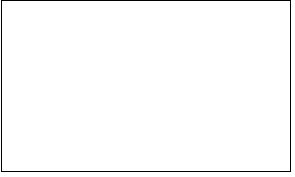
\includegraphics{figs/grabs.pdf}
% \end{graphicalabstract}

% Research highlights
%\begin{highlights}
%\item Research highlights item 1
%\item Research highlights item 2
%\item Research highlights item 3
%\end{highlights}

% Keywords
% Each keyword is seperated by \sep
\begin{keywords}
quadrupole exciton \sep polariton \sep \WGM \sep \BEC
\end{keywords}

\maketitle

\section{Introduction} %% {{{
%\subsection{Motivation}

% Motivação: contextualização do problema ou da necessidade que motivou o trabalho. Essa seção deve preparar o leitor para a <Pergunta da Pesquisa>

According to the World Health Organisation (WHO), there are at least 2.2 billion people with some visual impairment degree \cite{world2019world}. Among them, 43,3 million are classified as blind and 295 million have moderate or severe vision impairment. In order to be fully integrated into our society, they rely on assistive devices, such as canes, braille speakers, among others \cite{bourne2021trends}. 

Although a range of products has already been proposed, incorporating different features, they do not entirely fulfill their aim. Among the problems, of the solutions available in the market, are the lack of practicality and portability, invasive and requiring too much effort to learn \cite{lozano2009electrotactile}.

The difficulty of using or learn how to use a device could be avoided if concepts from Human Factors, or Ergonomics, were analysed during the product’s development, using appropriate methods. The early application of these methods and tests could be a gamechanger for the success of the product's user experience \cite{wolf2019towards}.

Motivated by the dissatisfaction of blind people with the currently available products, this paper starts from the hypothesis that a human-factors-centred design of assistive devices for blind and visually impaired people (BVIs) requires the involvement of BVIs in the design process in order to evaluate the product under design. The user has to test the product under development to provide feedback for the design team to improve the product.

In order to approach this problem, this work proposes using virtual reality (VR) as a tool for creating virtual environments, where proof of concepts or prototypes of assistive devices could be tested by BVIs. VR can be used to create specific, immersive and interactive situations that could help the user to learn and train \cite{farrell2018learning}, and the the developers to create more user-friendly products.

In a virtual environment, as long as the BVI is wearing a locating system, s/he can navigate the environment. Any information about the scenario, such as the position of objects and their distances to the user, is known and could be extracted from the virtual platform. As a consequence the designer can test different ways of translating this information into inputs before actually implementing a prototype of the assistive device, providing a flexible, safe and easy way to have it evaluated by different users.

%\section{Virtual reality in the design process}
\label{sec:vr_cabin}
The use of virtual reality for design purposes is not new. The cabin design process is often said to be complex because it involves several stakeholders, each with his/her own set of preferences and requirements. \cite{moerland2021application} proposed to anticipate the involvement of the final users based on co-design. In their proposal, the users can influence the product's development from the beginning. However, for the involvement to happen, a communication channel needed to be established, and it was done using virtual reality. The use case showed some benefits and disadvantages of using virtual reality. The virtual reality helped to bring the client closer to the design team, allowing them to draw quick sketches in brainstorming gatherings. It was associated with a steep learning curve for the designers. Among the disadvantages, it was considered a high-cost tool, and its use for a long time was associated with nausea.

%\section{Virtual reality for BVI users}
\label{sec:vr_without_vision}
Motivated by the popularization of virtual reality technology, \cite{siu2020virtual} developed a white cane to be used by BVI users in a virtual environment. Their purpose was to make virtual reality applications available for BVI users. In order to evaluate their proposal, the authors performed an experiment where the participants had to play a “scavenger hunt” using an HTC Vive system. Among the relevant findings of \cite{siu2020virtual} is that not all the participants reacted the same to a particular stimulus. The vibration of the cane was considered confusing by some participants, while others were familiar with it. Another interesting observation was that, similar to what happens in the real world, it was easier for the participants to navigate in larger areas than in tight spaces. Moreover, the authors observed that the participants focused their attention on the primary task, without freely exploring the environment, which might have impacted the low time to achieve the goal and the low number of obstacle hits. 

%\section{Augmented reality for BVI users}
\label{sec:ar_without_vision}
\cite{kirner2011using} raised two questions, "How can blind people learn 3D concepts aiming to be able to convert explored 3D environments into pictures?" and "How can we develop a spatial audio tutor with augmented reality technology to make easy the understanding of 3D concepts by blind people?" and used not using virtual reality technology but augmented reality to answer them. They developed a augmented reality application to be a tutor for BVI users. The application used allowed BVI users to play audio streams that were associeated with spatial positions. The users learned 3D concepts and also were able to  perceive, understand and produce embossed pictures representing real and imaginary 3D scenes. Also they were able to understand descriptions of 3D scenes described by non-BVI people. The authors believe that this application can be evolved to explain other concepts such as colors, transparency, shades, etc.

%\section{Information for BVI navigation}
\label{sec:bradley_dunlop}
Bradley and Dunlop published two works (\citeyear{bradley2002investigating,bradley2005experimental}) about how BVI navigates and how much it is similar or different to how a sighted person navigates. The first work of Bradley and Dunlop was published in \citeyear{bradley2002investigating} and discussed which type of information BVI uses to navigate in an environment and how it compares to sighted people. The second they compared the perceived workload of BVI participants and sighted participants when they navigate using user-tailored information created with the results of the previous experiments \cite{bradley2005experimental}. The results showed that BVI users reached landmarks significantly quicker when given the information made for that group, but still longer than sighted users. Also it showed that BVI participants systematically have a higher workload than sighted participants and that BVI users did have a higher workload when guided by orientations provided by sighted people, as well as the sighted participants did with orientations from BVI.

%\subsection{Mental Workload (MWL)}
\label{sec:mental_workload}
Mental workload is one of the main concepts studied in Human Factors \cite{stanton2004handbook}. The mental workload is similar to the physical workload but refers to the mental capacity necessary to perform a task. Each human being has a finite mental capacity. When the mental demand is higher than the operator's capacity, the person needs to adapt to finish the task, or the overall performance of the task is compromised. Otherwise, if the mental workload is too low, the operator may get bored and easily distracted and could also fail or not process the task's information. The mental workload is not a quantitative resource or something that one can directly measure, but several different techniques have been proposed in the literature to infer it and they can be: techniques based on task performance, techniques based on physiological measures and techniques based on subjective questionnaires.
        
%\begin{figure}[!htb]
    \centering

    \tikzstyle{arrow} = [rounded corners, line width = 1mm, ->]
    
    \resizebox{0.85\width}{!}{
    \begin{tikzpicture}[node distance=1cm]
        
        \node (mwl) {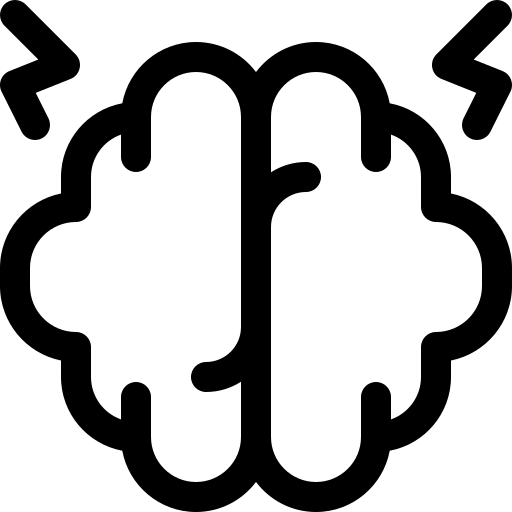
\includegraphics[width=.15\textwidth]{Fundamentação/Carga Mental/mwl.png}}
        node(t_mwl)[below of = mwl,yshift=-0.75cm] {Mental}
        node(t_mwl2)[below of = t_mwl,yshift=0.5cm] {workload};
        
        \node (demand) [above of=mwl, xshift=3cm, yshift=2.5cm] {\input{Fundamentação/Carga Mental/demand}}
        node(t_demand)[below of = demand,yshift=-0.75cm] {Task}
        node(t_demand2)[below of = t_demand,yshift=0.5cm] {Demand};
        
        \node (capacity) [above of=mwl, xshift=-3cm, yshift=2.5cm] {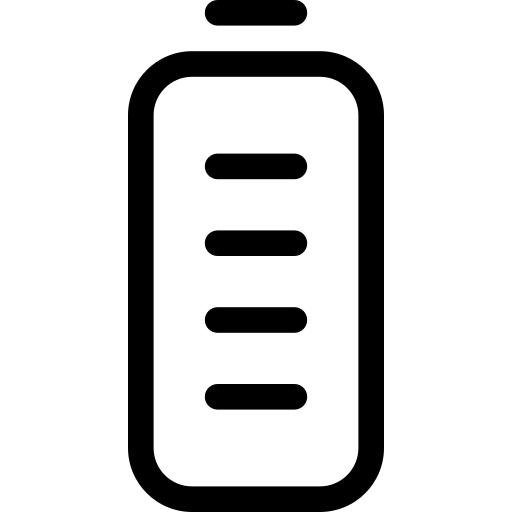
\includegraphics[width=.15\textwidth]{Fundamentação/Carga Mental/full-battery.png}}
        node(t_capacity)[below of = capacity,yshift=-0.75cm] {Mental}
        node(t_capacity2)[below of = t_capacity,yshift=0.5cm] {Capacity};
        
        \node (tasks) [left of=mwl, xshift=-4cm, yshift=-6cm] {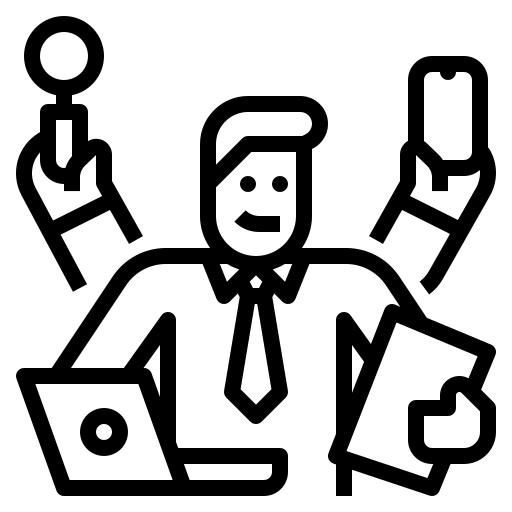
\includegraphics[width=.15\textwidth]{Fundamentação/Carga Mental/multitasking.png}}
        node(t_tasks)[below of = tasks,yshift = -0.75cm] {Primary and} 
        node(t_tasks2)[below of = t_tasks,yshift = 0.5cm] {secondary tasks};
        
        \node (physiological) [below of=mwl, yshift=-5cm,] {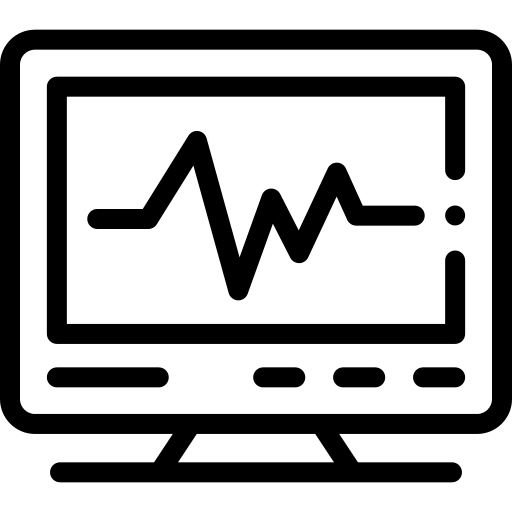
\includegraphics[width=.15\textwidth]{Fundamentação/Carga Mental/physiological.png}} 
        node(t_physiological) [below of = physiological, yshift = -0.75cm]{Physiological}
        node(t_physiological2) [below of = t_physiological, yshift = 0.5cm]{measurements};
        
        \node (subjective) [right of=mwl, xshift=4cm, yshift=-6cm] {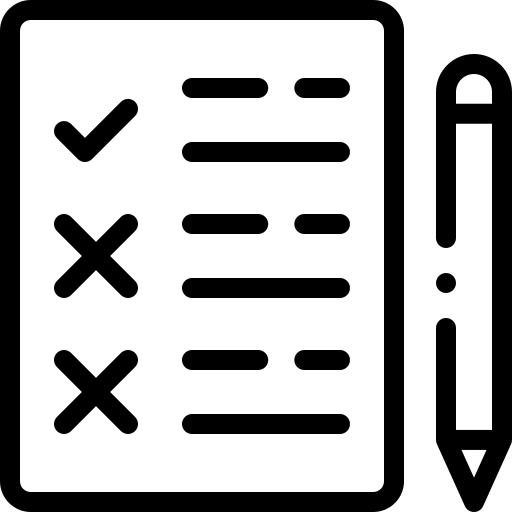
\includegraphics[width=.15\textwidth]{Fundamentação/Carga Mental/subjective.png}}
        node(t_subjective) [below of = subjective, yshift = -0.75cm]{Subjective} 
        node(t_subjective2) [below of = t_subjective, yshift = 0.5cm]{measurements};
    
    
        \draw [arrow] (t_mwl2.south) to ++(0,-0.75) to +(-5,0) to (tasks.north);
        \draw [arrow] (t_mwl2.south) to (physiological.north);
        \draw [arrow] (t_mwl2.south) to ++(0,-0.75) to +(5,0) to (subjective.north);
        \draw [arrow, sharp corners] (capacity.east) to +(1.6,0) to (mwl.north);
        \draw [arrow, sharp corners] (demand.west) -- +(-1.35,0) to (mwl.north);
    
        
    \end{tikzpicture}
    }
    \caption{A overview of mental workload and the techniques to infer it.}
    \label{fig:mwl_overview}
\end{figure}    

%\subsubsection*{Techniques based on task performance}
%\label{subsec:task_performance}

%If the mental workload influences the task performance, it would be possible to infer it using the performance's variation of a task. Because there are cases where the user's mental capacity is too high for only one task, a common approach is to add a secondary task. In this case, the user is asked to maintain a good performance level and still try to execute both tasks. Both tasks should use the same skills \cite{stanton2004handbook, sanders1998human}.
%
%For example, an experiment to assess mental workload in a flight simulator may use two tasks. The primary task is to fly the aircraft while maintaining a performance level. The second is something simple, like mentally summing two random numbers that appear on the screen. If the numbers' sum is odd, the pilot should press the left arrow key on the keyboard, otherwise should press the right arrow key. If the pilot's performance in the secondary task is too low, it means that the mental demand from the first task is too high to pay attention to the second task \cite{mohanavelu2020cognitive}.
%
%%    \item Physiological measures;
%\subsubsection*{Techniques based on physiological measurements}
%%\label{subsec:physiological_measures}
%
%Many physiological measurements can be used to assess mental workload. The most common ones are heart and brain activity \cite{chakladar2020eeg, orlandi2018measuring}, skin conductance, eye movement and pupillary contraction \cite{stanton2004handbook, rodriguez2015pupillometry}. These measurements are considered an user-unbiased assessment technique \cite{fallahi2016effects}. It is recommended to evaluate them alongside another method, as they can be influenced by unknown variables and external factors. Some techniques use heart activities, obtained from an electrocardiogram (ECG) sensor, and electrodermal activity, obtained from a galvanic skin response (GSR) sensor, as physiological measurements to assess mental workload.
%
%The electrocardiogram (ECG) is a recording of the heart's electrical activity. From it, it is possible to determine the intervals between heartbeats and the corresponding frequency (heart rate, HR). Another common variable is the heart rate standard deviation (heart rate variability, HRV) \cite{cain2007review}. The heart activity is controlled by the sympathetic and parasympathetic nervous systems \cite{stanton2004handbook}. During a task, the heart activity changes with the mental demand of the task. The heart rate is expected to increase with the mental workload, while the heart rate variability is expected to decrease. These are consequences of two reactions in our system when in a mental demand situation \cite{stanton2004handbook}: a decrease in the parasympathetic nervous system activity and an increase in sympathetic nervous system activity. The ECG is a simple and non-invasive sensor used in many experiments to evaluate mental workload and other human factors' \cite{mohanavelu2020cognitive, mansikka2016fighter, zhang2014detection}.
%%(DEFINIR MELHOR)
%
%The skin electrodermal activity is affected by the person's sweating and the level of moisture in the environment. It can be used to reveal changes in our sympathetic system \cite{nourbakhsh2012using, shi2007galvanic}. It has been used in the literature as an assessment technique for stress and arousal \cite{nourbakhsh2012using, stanton2004handbook, shi2007galvanic}, the usability of human-computer systems \cite{shi2007galvanic} and also mental workload \cite{zhang2014detection, borghini2014measuring}.
%
%\subsubsection*{Techniques based on subjective questionnaires}
%%\label{subsec:subjective_measures}    
%
%The use of subjective questionnaires to assess mental workload has been extensively discussed in the literature \cite{sanders1998human, stanton2004handbook}. The questionnaires can be unidimensional or multidimensional. The unidimensional questionnaires are more straightforward by provide only a general workload score.     Examples of multidimensional questionnaires are the Subjective Workload Assessment Technique (SWAT) and the NASA Task Load Index (NASA-TLX). SWAT decomposes the mental in three dimensions: time load, mental effort load, and psychological stress. NASA-TLX, a questionnaire created by \cite{hart1988development}, uses six dimensions, as described in Table \ref{tab:nasa_dimensions}. These questionnaires were proposed to evaluate only one task/activity. If the user has performed two tasks (a primary and secondary task), he/she should be oriented to answer about the primary task, not a combination of both \cite{sanders1998human}.
%
%\begin{table}[htb]
%    \centering
%    \caption{NASA-TLX dimensions and the description of each dimension. \cite{stanton2004handbook}.}
%    \label{tab:nasa_dimensions}
%    \begin{tabular}{|l|l|}
%
%        \hline
%        \textbf{Dimension}   & \textbf{Explanation}                                                                                                                                                       \\ \hline
%        Mental demand (MD)   & \begin{tabular}[c]{@{}l@{}}The mental and perceptive activity\\ demanded by the task (chose, decide,\\ think, calculate, search, etc.).\end{tabular}                       \\ \hline
%        Physical demand (PD) & \begin{tabular}[c]{@{}l@{}}The physical activity demanded by\\ the task (pull, lift, spin, drag, etc.).\end{tabular}                                                       \\ \hline
%        Temporal demand (TD) & \begin{tabular}[c]{@{}l@{}}The time pressure felt by the user.\\ A rating the leverages the time \\ available and the time necessary to\\ completed the task.\end{tabular} \\ \hline
%        Performance (PE)     & \begin{tabular}[c]{@{}l@{}}The user's satisfaction with its \\ performance or result the task.\end{tabular}                                                                \\ \hline
%        Effort (EF)          & \begin{tabular}[c]{@{}l@{}}A rating of the effort necessary \\ to achieve that performance felt by\\ the user.\end{tabular}                                                \\ \hline
%        Frustration (FR)     & \begin{tabular}[c]{@{}l@{}}A rating of stress, annoy or irritation\\ felt by the user throughout the task.\end{tabular}                                                    \\ \hline
%    \end{tabular}
%\end{table}
%
%Finally, it is essential to highlight that, to have a comprehensive evaluation of the mental workload, not to choose only one technique, but to combine techniques from the three classes (task performance, physiological measurements and subjective questionnaires). Mental workload is multidimensional and can reflect partially or differently in each technique \cite{sanders1998human}.

%\subsection{Situation Awareness (SA)}
\label{sec:situation_awareness}
%Situation awareness can be defined as “the perception of the elements within a volume of time and space (Level 1), the comprehension of their meaning (Level 2), and the projection of their status in the near future (Level 3)” as illustrated in Figure \ref{fig:sa_overview}. One example is when an air traffic controller looks at a radar display (Level 1). He/she seeks to understand the aircraft's position and speed (Level 2) and then predict its position in the near future, 5, 10 or 15 minutes after (Level 3) \cite{sanders1998human}. Similarly, when a pilot reads the cockpit panel (Level 1) and understands their data (Level 2) then he/she can predict the next reading of that same instrument or some other status of the aircraft after a couple of minutes (Level 3).

%\begin{figure}[!htb]
    \centering
    \tikzstyle{arrow} = [rounded corners, line width = 1mm, ->]

    \resizebox{0.85\textwidth}{!}{
    \begin{tikzpicture}[node distance=3.3cm]
        \centering
        
        \node (info) [fill=white] {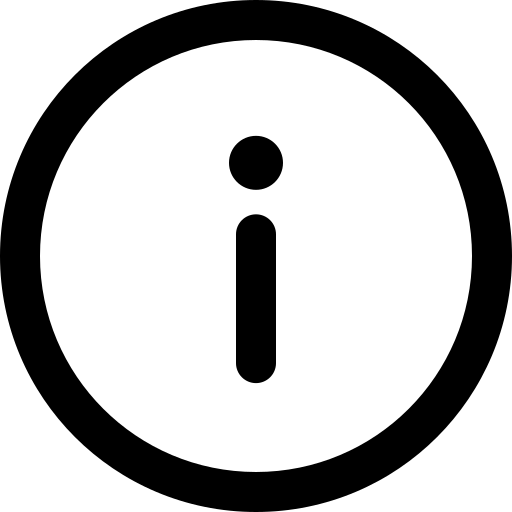
\includegraphics[width = 0.20\textwidth]{Fundamentação/Percepção situacional/information.png}}
        node(t_info)[below of = info,yshift=1.3cm] {\Large Information};
        
        \node (arrow) [right of=info, xshift=7.0cm, yshift = -0.5cm] {\input{Fundamentação/Percepção situacional/seta}};
        
        \node (perception) [right of=info, xshift=2.5cm, draw, line width=2mm] {\input{Fundamentação/Percepção situacional/perception}}
        node(t_perception)[below of = perception, yshift=0.9cm] {\Large 1st Level}
        node(t_perception2)[below of = t_perception, yshift=2.5cm] {\Large Perception};

        \node (comprehension) [right of=perception, xshift=0.25cm, draw, line width=2mm] {\input{Fundamentação/Percepção situacional/comprehension}}
        node(t_comprehension)[below of = comprehension, yshift=0.9cm] {\Large 2nd Level}
        node(t_comprehension2)[below of = t_comprehension, yshift=2.5cm] {\Large Comprehension};

        \node (projection) [right of=perception, xshift=3.75cm, draw, line width=2mm] {\input{Fundamentação/Percepção situacional/projection}}
        node(t_projection)[below of = projection, yshift=0.9cm] {\Large 3rd Level}
        node(t_projection2)[below of = t_projection, yshift=2.5cm] {\Large Projection};

        \node (decision) [right of=projection, xshift=5.0cm] {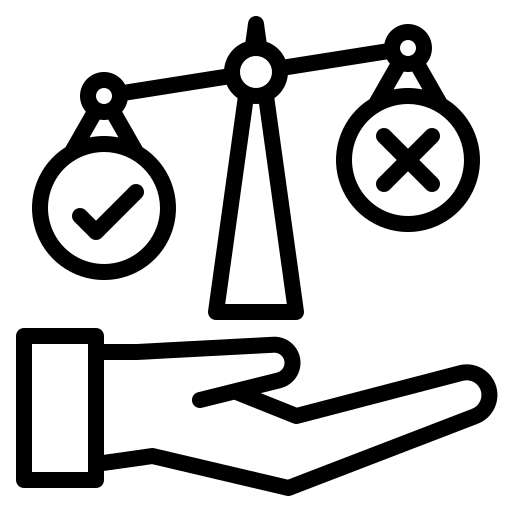
\includegraphics[width = 0.30\textwidth]{Fundamentação/Percepção situacional/decision.png}}
        node(t_decision)[below of = decision, yshift=0.5cm] {\Large Decision}
        node(t_decision2)[below of = t_decision, yshift=2.5cm] {\Large making};

    \end{tikzpicture}
    }
    \caption{An overview of situation awareness and the SAGAT.} %and the methods to infer it
    \label{fig:sa_overview}
\end{figure}

The term “situation awareness” was first proposed for the Aeronautics domain and today is considered a key factor for designing complex and dynamic systems from other domains, such as automotive, medical and nuclear \cite{endsley1995measurement}. It can be defined as “the perception of the elements within a volume of time and space (Level 1), the comprehension of their meaning (Level 2), and the projection of their status in the near future (Level 3)” \cite{sanders1998human}. It is an essencial factor to make sure that the user will be capable to make important decisions correctly and achieve high-performance \cite{endsley1988design, endsley2018automation}. As it is for the mental workload, situation awareness is not a quantitative subject. The most common way to measure it is using subjective techniques, among which one of the most famous is the Situation Awareness Global Assessment Technique (SAGAT). It was proposed by \cite{endsley1988design} and is based on how the information is processed inside the user’s mind.

%The test application is made by freezing the operator activity, usually made in a simulation environment, and then asking the user some questions that were previously defined based on the user's activity. These questions should be as similar as possible to how the person thinks when reasoning about the situation to avoid extra effort in understanding it \cite{stanton2004handbook}.  Although freezing the activity may sound troublesome, empirical work has shown that it does not interfere with the user performance and the user memory can withstand a break for as long as 5 to 6 min \cite{endsley1988design}.


%\section{Co-Design}
\label{sec:co_design}
Co-design, or collaborative design, refers to a design process in which individuals of the design team have different backgrounds or bring different experiences, which can be essencial for the product under design. It is based on good communication and information sharing among the team \cite{chiu2002organizational}.

%\cite{kleinsmann2006understanding} provides the following definition:.
%
%\begin{quote}
%    \textit{"Collaborative design is the process in which actors from different disciplines share their knowledge about both the design process and the design content. They do that to create a shared understanding of both aspects, to be able to integrate and explore their knowledge and to achieve the larger common objective: the new product to be designed."} \cite{kleinsmann2006understanding}.
%\end{quote}
%
%This definition emphasizes two critical aspects of co-design: knowledge sharing and integration. According to \cite{kleinsmann2006understanding} knowledge is the data after the receiver's understanding or translating process, in a state that is possible to record or register, so that the person can remember and use it later. During the collaborative design, ideas, facts or concepts are exchanged between the actors. This exchange is a fundamental part of the co-design process since it is responsible for the growth of each individual's knowledge. Once the knowledge is shared among the actors, they can use it when performing their tasks, resulting in knowledge integration \cite{kleinsmann2006understanding}.

This paper's main goal is the use of virtual reality as a tool for evaluating proofs of concept of assistive devices for blind and visually impaired people from a human-factors perspective. The purpose is to provide a flexible and easily configured way of testing different concepts of assistive devices in order to support an agile and user-centered development.

This goal is related to the following research questions, which are investigated in this work:

\begin{itemize}
   \item Is it possible to evaluate and compare concepts of assistive devices from a human factors perspective in a virtual environment? What are the main limitations of the use of a virtual reality environment? \label{itm:obj_first}
   \item Do non-BVI users, when deprived of their vision, similarly evaluate assistive devices as BVI users? \label{itm:obj_second}
\end{itemize}

% Delimitação da pesquisa: é o recorte do seu trabalho

The concepts of assistive devices presented as part of this work are used only as examples for investigating the research questions presented. The challenges related to their full development up to high Technology Readiness Levels (TRLs), as well as their feasibility as commercial products, are out of the scope of this work.

% Estrutura do texto

\subsection*{Structure of the text}

The next Section of this paper are organized as follows.

Section \ref{ch:metodologia} details the proposal of this paper describing how virtual reality could be used to integrate BVI users into the design process of assistive design. It illustrates the proposed method by applying it to evaluate three different assistive devices (audio guide, virtual cane and haptic belt), as well as their mixed-use, in the environment of a hospital reception. 

Section \ref{ch:resultados} describes the experiment designed to evaluate the paper's proposal and analyses the results in order to investigate the research questions of Section \ref{sec:objetivos}

Finally, section \ref{ch:conclusao} summarizes the main conclusions of this work and discusses future work.


%% ---------------------------
%% Methodology
%% ---------------------------
\section{Material and methods}
\label{ch:metodologia}
This chapter describes the method proposed in this work for evaluating assistive devices using virtual reality. The method is organized into 5 phases as illustrated in Figure \ref{fig:diag_metodologia}.


%\tikzstyle{start} = [rectangle, rounded corners, minimum width=4cm, minimum height=1.0cm,text centered, draw=black, fill=white!30, text width=3cm]
\tikzstyle{process} = [rectangle, minimum width=4cm, minimum height=1.0cm, text centered, draw=black, fill=white!30, text width=3.5cm]
\tikzstyle{decision} = [diamond, minimum width=3.5cm, minimum height=1.0cm,  text centered, text width=3.5cm, draw=black, fill=white!30]
\tikzstyle{arrow_flow} = [ccmDBlue, rounded corners, line width = 2mm, ->]
\tikzstyle{arrow_return} = [ccmRed, rounded corners, line width = 2mm, ->]

\begin{tikzpicture}[node distance=2cm]
    \centering
    \node (start) [start] {Collect the ECG Data};
    \node (read) [process, below of=start,yshift=-0.5cm] {Read the GSR file};
    \node (average) [process, aspect=2.5, below of=read, yshift=-0.5cm] {Calculate the average};
    %\node (std) [process, aspect=2.5, below of=average, yshift=-0.5cm] {Calculate the standard deviaton};
    
    \draw [arrow_flow] (start.south) -- (read.north);
    \draw [arrow_flow] (read.south) -- (average.north);
    %\draw [arrow_flow] (average.south) -- (std.north);
    %\draw [arrow_flow] (std.south) -- (findPeaks.north);
    
\end{tikzpicture}
\begin{figure*}[!htb]
    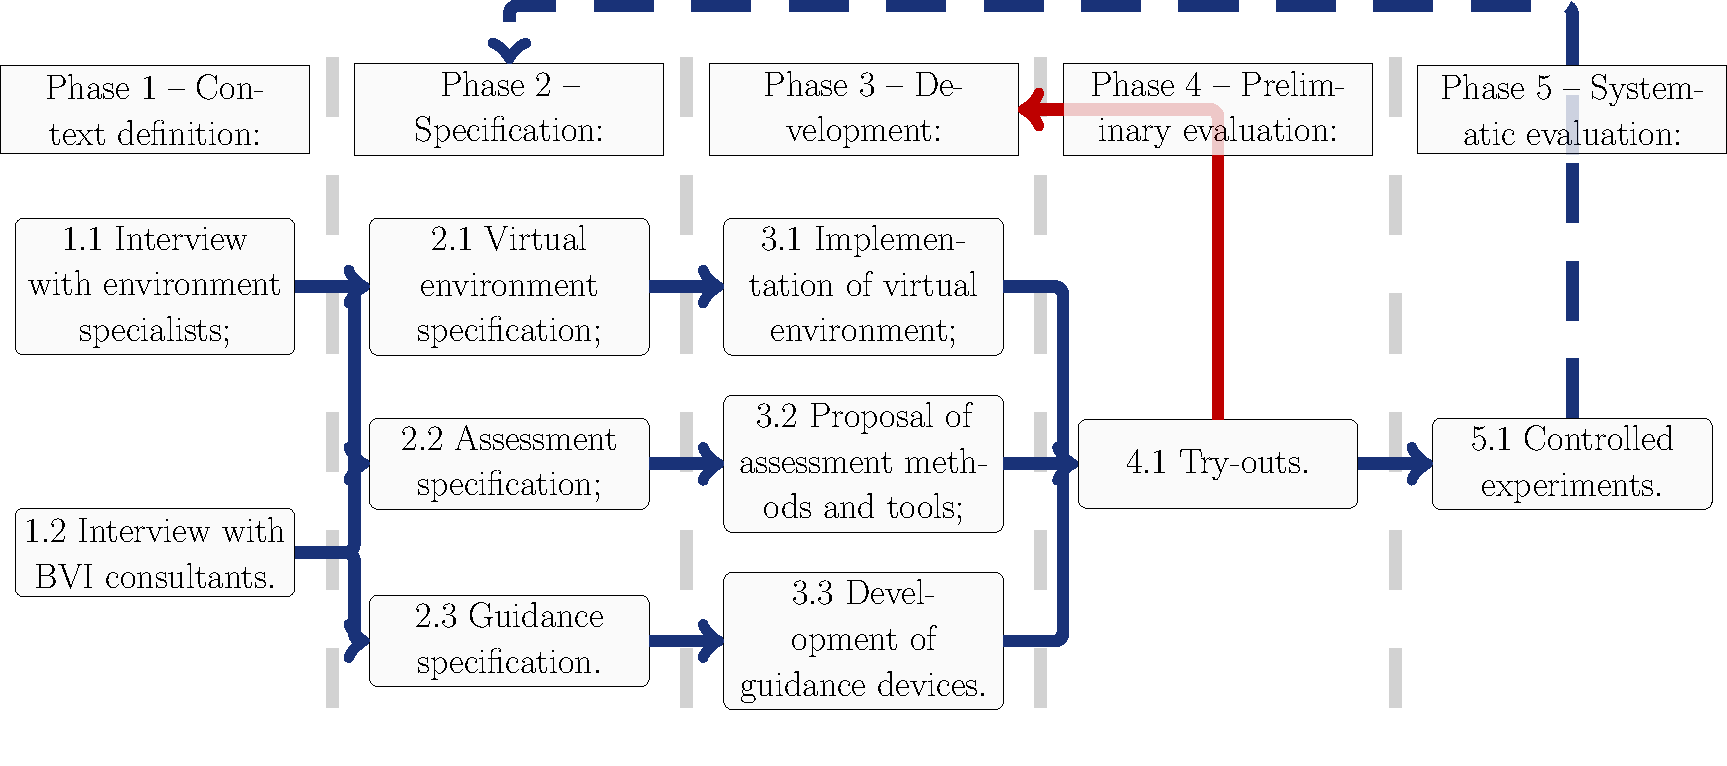
\includegraphics[width = \linewidth]{2 - Metodologia/metodologia.pdf}
    \caption{Method's diagram}
    \label{fig:diag_metodologia}
\end{figure*}

%% ---------------------------
%% 1 Phase
%% ---------------------------

The first phase is the context definition. It consists of defining the main features of the environment in which the assistive device will be used, based on interviews from hospital's specialists from São José dos Campos. It also includes a step for understanding the limitations of the current assistive devices and defining the main features of assistive devices to be designed. This last step is based on interviews with two BVI users, one that is blind since 13 years old and another that has Usher's disease.

%% ---------------------------
%% 2 Phase
%% ---------------------------

In the second phase, the information collected through the interviews of Phase 1 is used to make critical decisions about the virtual environment where the evaluation of the assistive devices will be carried out. It is also used to define which human factors should be assessed. Finally, it contributes to define the guidance devices that should be implemented in the assistive devices.

%% ---------------------------
%% 3 Phase
%% ---------------------------

    The third phase is dedicated to developing the virtual environment, the evaluation tools and techniques, and the first proof of concept of the assistive devices, which should be integrated into the virtual environment for testing.

    %% ---------------------------
    %% Virtual Environment
    %% ---------------------------
    \subsection*{Virtual Environment}
    The virtual reality environment was developed using the Unity3D platform and the implementation should be followed by preparing the corresponding physical space to perform the test campaign. Following the recommendations from the BVI interviews, typical reception furniture was placed in the virtual environment as illustrated in Figure \ref{fig:task_diagram}. Sounds were also used to increase the feeling of immersion and indicate to the BVI participant where the reception desk was located. The participant navigation through the reception was composed of 4 tasks, also illustrated in Figure \ref{fig:task_diagram}:

    \begin{enumerate}
        \item Clean the hands at the sanitizer totem (COVID-19 procedures);
        \item Go to the reception desk to receive a queue number;
        \item Go to the waiting area and wait for the number calling;
        \item Leave the room when called.
    \end{enumerate}

    \begin{figure}[!htb]
        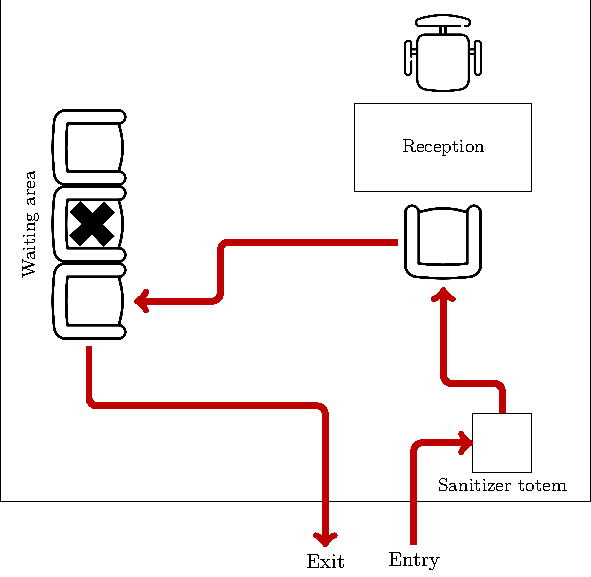
\includegraphics[width = \linewidth]{2 - Metodologia/caminho.pdf}
        \caption{Scheduled task of the experiment and their order.}
        \label{fig:task_diagram}
    \end{figure}

    Figure \ref{fig:ve_phot} shows the virtual environment created in Unity3D and the corresponding real environment assembled at the CCM entrance hall. 

    \begin{figure}[!htb]
        \centering
        \begin{subfigure}[b]{0.75\linewidth}
            \centering
            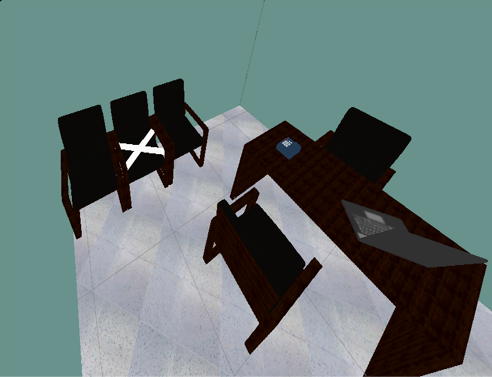
\includegraphics[width=\linewidth]{2 - Metodologia/VE.png}
            \caption{Virtual environment screenshot}
            \label{fig:ve_photo}
        \end{subfigure}
        \hfill
        \begin{subfigure}[b]{0.75\linewidth}
    %\end{figure}    
    %\begin{figure}[!htb]
            \centering
            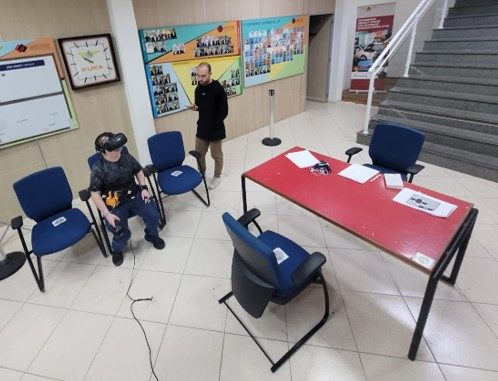
\includegraphics[width=\linewidth]{2 - Metodologia/RE.jpg}
            \caption{   }
            \label{fig:re_photo}
        \end{subfigure}
        \caption{Environment comparisson}
        \label{fig:ve_re}
    \end{figure}


    %% ---------------------------
    %% Human Factors techniques
    %% ---------------------------
    \subsection*{Human Factors techniques}
    The assessment should evaluate workload, situation awareness and the user's impressions using:

%\begin{enumerate} [label = \Alph*)]
%    \item Task Performance;
%\end{enumerate}
%    
%In the hospital reception scenario, the proposed measurement related to BVI performance is the number of times the BVI user hits the furniture in the virtual environment during the tasks' execution.

    \begin{enumerate} [1.]
        \setcounter{enumi}{0}
        \item Workload;
    \end{enumerate}

    Following the recommendations from the review of literature, the workload is estimated using two approaches:
    \begin{itemize}
        \item Physiological measures obtained from an ECG (Electrocardiogram) sensor and a GSR (Galvanic Skin Response) sensor;
        \item NASA-TLX (National Aeronautics and Space Administration Task Load Index) subjective questionnaire.
    \end{itemize}

    \begin{enumerate} [2.]
        \setcounter{enumi}{1}
        \item Situation awareness;
    \end{enumerate}

    A modified SAGAT (Situation Awareness Global Assessment Technique) questionnaire is used to evaluate the BVI situation awareness.
    As original idea from \cite{endsley1988design}, the proposed version is based on 3 levels of situation awareness:
    
    \begin{enumerate}[Level 1.]%[leftmargin = 6em, label = Level \arabic* -- ]
        \item Perception
        
        It aims to evaluate if the user can perceive the environment surrounding him/her.

        \item Comprehension

        After the user answer about an detected object, he/she is asked to point to where the object is located. 

        \item Projection
        
        This level is measured after every question that asks the location of an object. He/she is then required to answer how far he/she supposes that this object is
        
    \end{enumerate}      

    \begin{enumerate} [3.]
        \setcounter{enumi}{2}
        \item Devices evaluation;
    \end{enumerate}

    Finally, a questionnaire is proposed for evaluating the guidance devices. The questions were about the comfort, the sense of safety, the sense of confusion and on the precision that the manipulation of the device caused.

    %% ---------------------------
    %% Assistive Devices
    %% ---------------------------
    \subsection*{Assistive Devices}
    Four guidance methods were proposed to be evaluated in this work.
        
    \begin{enumerate} [1.]
        \item Audio guidance;
        
        The first method is audio guidance. Basically, in the course of the experiment, the participant could give two different voice commands: “What is around me?” and “Where is (something)?”. The answers of both commands was done with the interference of a member of the design team.  

        \item Vibration guidance with command – virtual cane;
        
        When using a white cane, the user points it to check nearby obstacles in a specific direction. The virtual cane has a similar way of functioning, but instead of connecting the user to the nearby object through the cane, it vibrates when it detects an obstacle in the direction the user pointed it.

        \item Vibration guidance without command – haptic belt
        
        The belt has appended 8 vibration units that vibrate accordingly to the direction and distance of the closest object around the user. The main differences between the virtual cane and the haptic belt is that the haptic belt checks 360° around the user. When objects are within a certain limit, it vibrates indicating to the user the direction of the closest object. 

        \item Mixture of audio and vibration guidance
        
        This option is implemented making the three options available to the user: audio guidance, haptic belt and virtual cane. 
    \end{enumerate}


The fourth phase provides a preliminary assessment of the devices through its unstructured experimentation by BVI consults. This preliminary assessment provides feedback for improving the device concept. The cycle of “try-out and improve device concept” can be repeated until the device concept is considered mature to be tested through a systematic set of controlled experiments.

The fifth phase consists of executing a campaign of controlled experiments, following the best practices of the DoE (Design of Experiments) discipline, and analysing the results. Concluded this phase, the results should provide information for the design team to decide between proceeding to the detailed design of the assistive devices or performing a new evaluation cycle.

In the case of this work, the proposed experiment consists of asking the participant to use five guidance methods: the audio guidance, haptic belt, virtual cane, mixed and, additionally, the device used daily by the BVI (e.g., white cane). Moreover, each participant should use each guidance method twice (“first visit” and “return visit”), in order to provide some information about how the guidance devices performs in new and known environments. In order to avoid the learning effect from one method to the other, five versions of the reception scene are developed, changing the position of the objects - one version to be used with each guidance method. The scene order is randomized for each participant.

Moreover, particularly in the case of this work, an additional round of tests is added to the experiment to investigate the differences between the evaluation performed by BVI users and sighted (non-BVI) users. For this purpose, the same experiment is repeated with a set of non-BVI users. The purpose is to investigate whether or not performing the analysis with non-BVI users could lead to different conclusions.

The experiment is organized in the following way:

\begin{itemize}
    \item Briefing:
    \item Execution of the experiment:
    \begin{itemize}
        \item Guidance method training;
        \item First visit and SAGAT questionnaire;
        \item NASA-TLX for the first visit;
        \item Return visit and SAGAT questionnaire;
        \item NASA-TLX for the return visit;
        \item Questionnaire about the guidance method.
    \end{itemize}
    \item Experiment's conclusion
\end{itemize}

As a result of the experiment, the following data are collected:

\begin{itemize}
    \item Answers to the NASA-TLX questionnaire;
    \item ECG and GSR signals;
    \item Answers to the SAGAT questionnaire;
    \item Answers to the guidance method questionnaire.
\end{itemize}

%% ---------------------------
%% Results
%% ---------------------------
\section{Results}
\label{ch:resultados}
%CAPÍTULO 4: ANÁLISE DOS RESULTADOS E DISCUSSÃO

%1. Elabore um parágrafo que introduz o capítulo: Este capítulo apresenta (descreva o objetivo do capítulo ...). É constituído de N seções a saber...
%2. Caso vc tenha aplicado a sua contribuição (modelo, produto, processo etc.) em um caso (empresa, laboratório, simulação etc.), apresente a descrição e análise dos resultados. Na seção de discussão cabem as análises de cenários What-If ou de sensibilidade. Exemplo: se o parâmetro X aumentar de N para N+1, o resultado poderia mudar de Y para Z?
%3. Elabore um parágrafo que conclui o capítulo e introduz o capítulo seguinte.

%The purpose of the experiment discussed in this chapter is to investigate the two research questions proposed for this work:
%
%\begin{itemize}%[leftmargin = 3.5em, label = $H_\arabic*$:]
%    \item Is it possible to evaluate and compare concepts of an assistive device from a human factors' perspective in a virtual environment? What are the main limitations of the use of a virtual reality environment?
%    \item Do non-BVI users, when deprived of their vision, similarly evaluate assistive device as BVI users?
%\end{itemize}

The described experiment was performed with the following groups and has an approval of the brazilian ethics commitee.:

\begin{itemize}
    \item Blind group: composed of 4 participants with ages varying from 26 to 56, all male, three of them graduated and one with ongoing graduation. 

    \item Sighted group: composed of 4 participants with ages varying from 22 to 31, three males and one woman, all graduated.
\end{itemize}

%In order to answer the two research questions, this chapter is organized in the following way. Section \ref{sec:results_obj_1} is dedicated to the first question and brings an analysis performed only with data from blind participants. Then, Section \ref{sec:results_obj_2} repeats the same analysis now with data from sighted participants and compares the results with those obtained from blind participants in order to answer the second research question.
%
%In both sections, 
The data analysis follows the following sequence:

\begin{itemize}
    \item Analysis of subjective questionnaires:
    \begin{itemize}
        \item NASA-TLX: %it aims at assessing the workload perceived by the user in six dimensions, including 'mental demand'. It is expected a decrease in the mental workload between the 'first' to the 'return' round. It is also expected that some guidance methods would differ regarding the required mental workload.
        \item Adapted SAGAT: %it aims at assessing the situation awareness and the user's mental map. It is expected that the SAGAT score would increase from the 'first' to the 'return' round. It is also expected that some guidance methods would differ regarding the required situation awareness provided to the user.
        \item Guidance method's questionnaire: %It assess the user experience with each method. It is also expected that some guidance methods would differ regarding the score received in this questionnaire.
    \end{itemize}
    \item Analysis of physiological sensors:
    \begin{itemize}
        \item ECG (Electrocardiogram): 
        
        Two features are extracted from the ECG signal, heart rate (BPM) and heart rate variance (SDNN).% The heart rate is expected to decrease slightly from the 'first' to the 'return' round, while the heart rate variance is expected to increase slightly.
        
        \item GSR (Galvanic Skin Response): %it aims at assessing the user workload and stress. It is expected that the GSR average would increase at every 'first' round and then a slight decrease in the 'return' round.
    \end{itemize}
\end{itemize}

\subsection{Evaluation of assistive device from a human factors' perspective in a virtual environment}
\label{sec:results_obj_1}

%\subsection{Subjective data}
\subsubsection{NASA-TLX}
\label{subsubsec:results_nasa_tlx_1}

The NASA-TLX provides two relevant pieces of information to the workload analysis. The first is the score attributed to the "mental demand" dimension and the second is the average obtained from NASA-TLX's six dimensions. The two analyses are presented in the next subsections.

\paragraph*{Analysis of the mental demand scale}\mbox{}\\


Figure \ref{fig:boxplot_md_blind_scene}  presents a boxplot of the mental demand score grouped by the methods. This figure shows that there may be two groups: one associated with lower demand, composed of base and audio, and another with higher demand, composed of haptic belt, virtual cane and mixture. It indicates that maybe a guidance method that uses vibration as input is not intuitive. Figure \ref{fig:boxplot_md_blind_rounds} presents a boxplot of the mental demand grouped by the rounds, confirming the general tendency to reduce the required "mental demand". 

\begin{figure}[!htb]
    \centering
    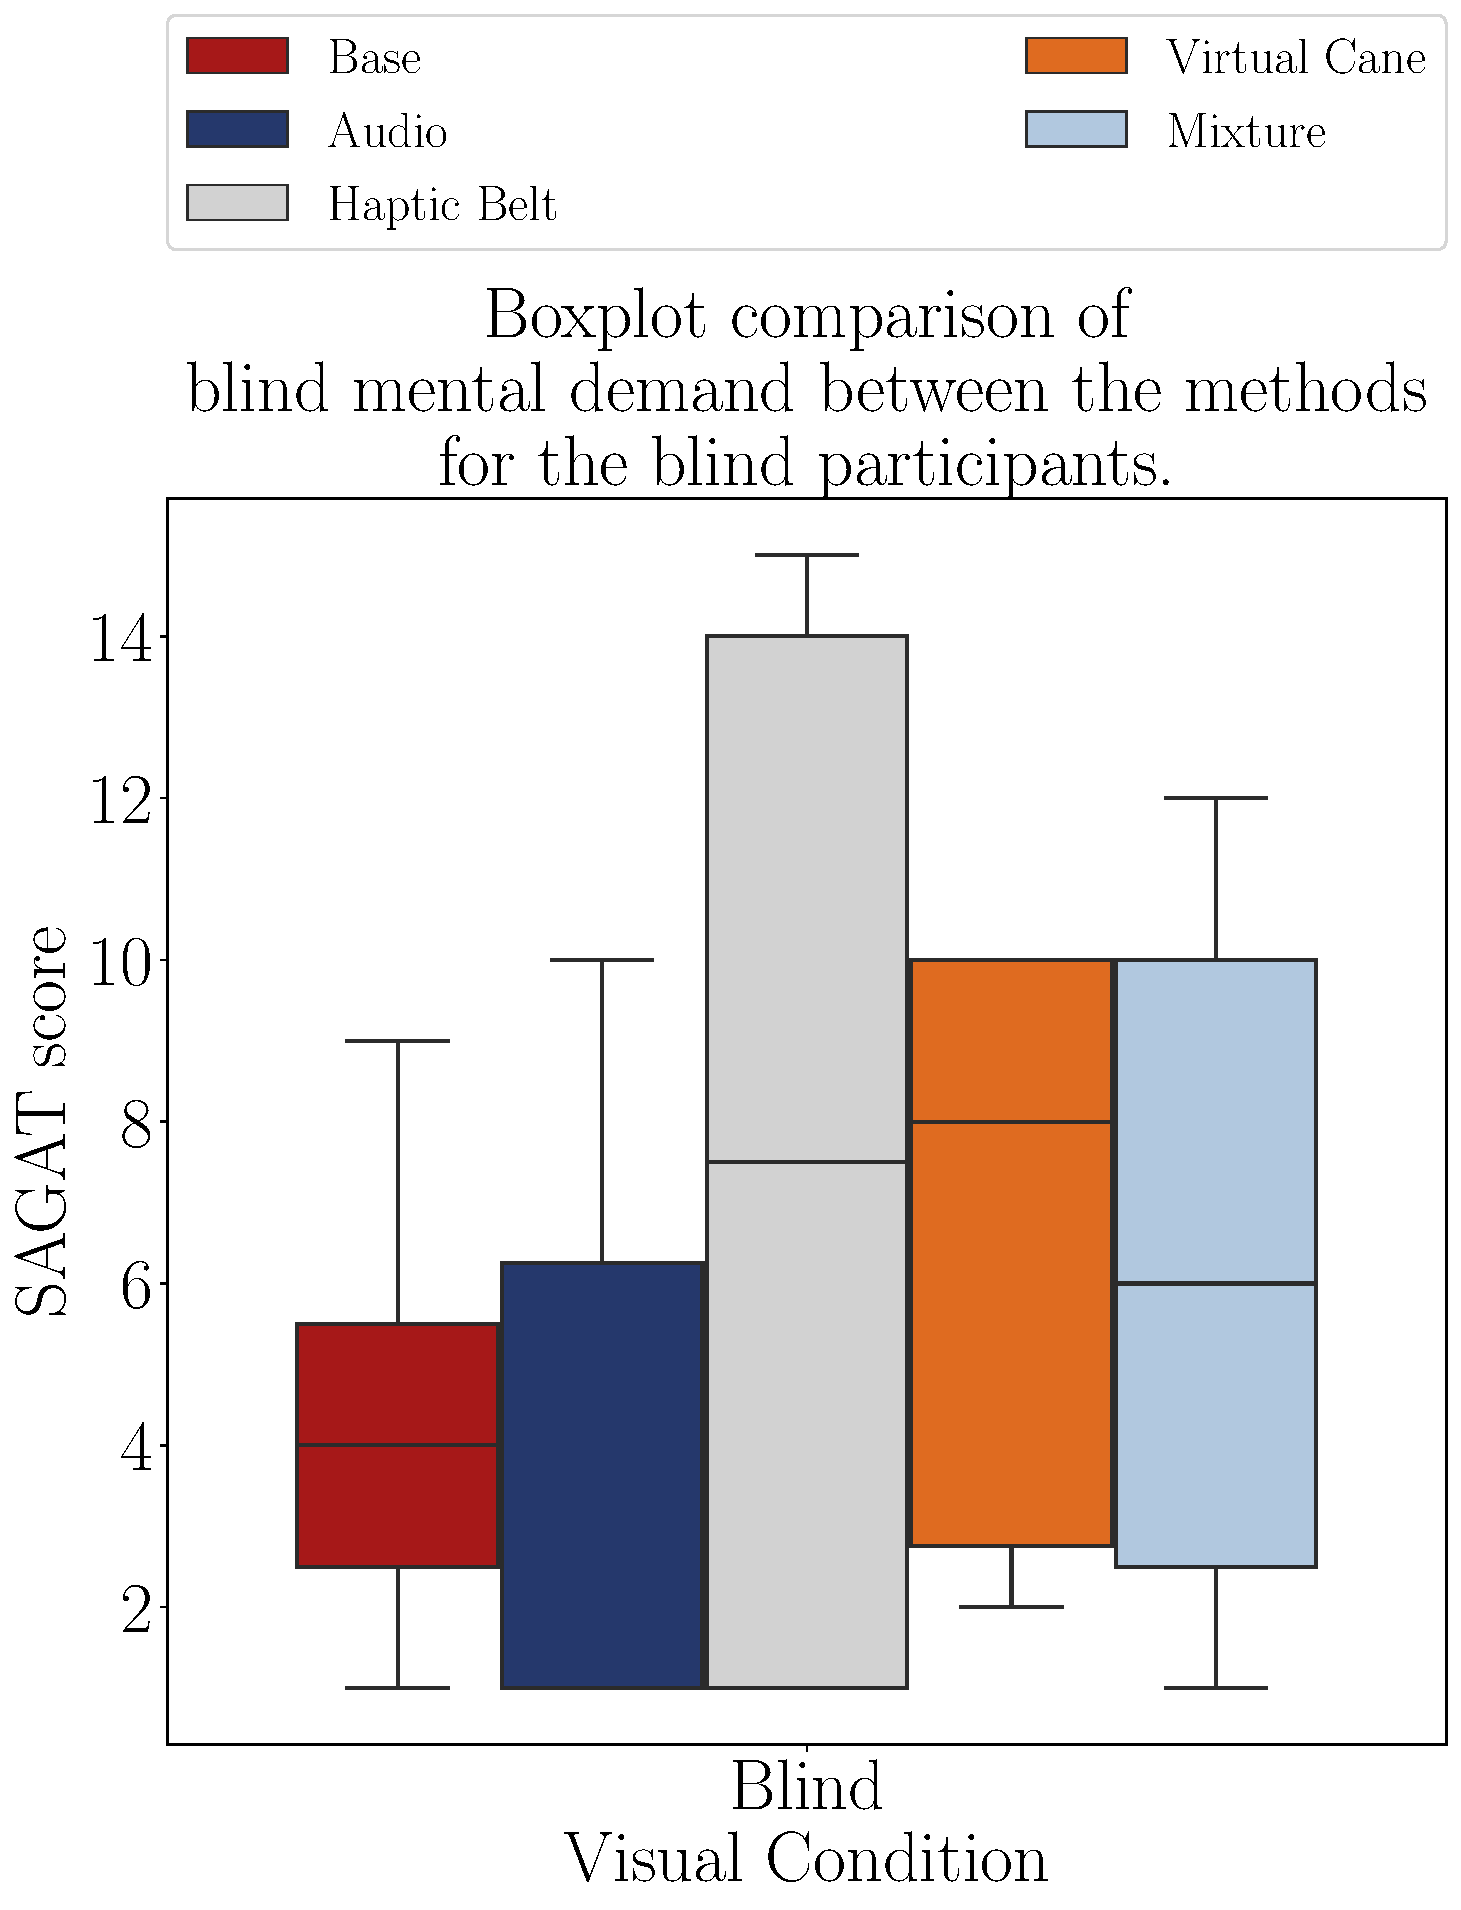
\includegraphics[width = 0.75\linewidth]{3 - Resultados/Figuras/boxplot_md_blind_scene.pdf}
    \caption{Boxplot of the mental demand of the blind participants grouped by the methods.}
    \label{fig:boxplot_md_blind_scene}
\end{figure}    
\begin{figure}[!htb]
    \centering
    %\vspace{3ex}
    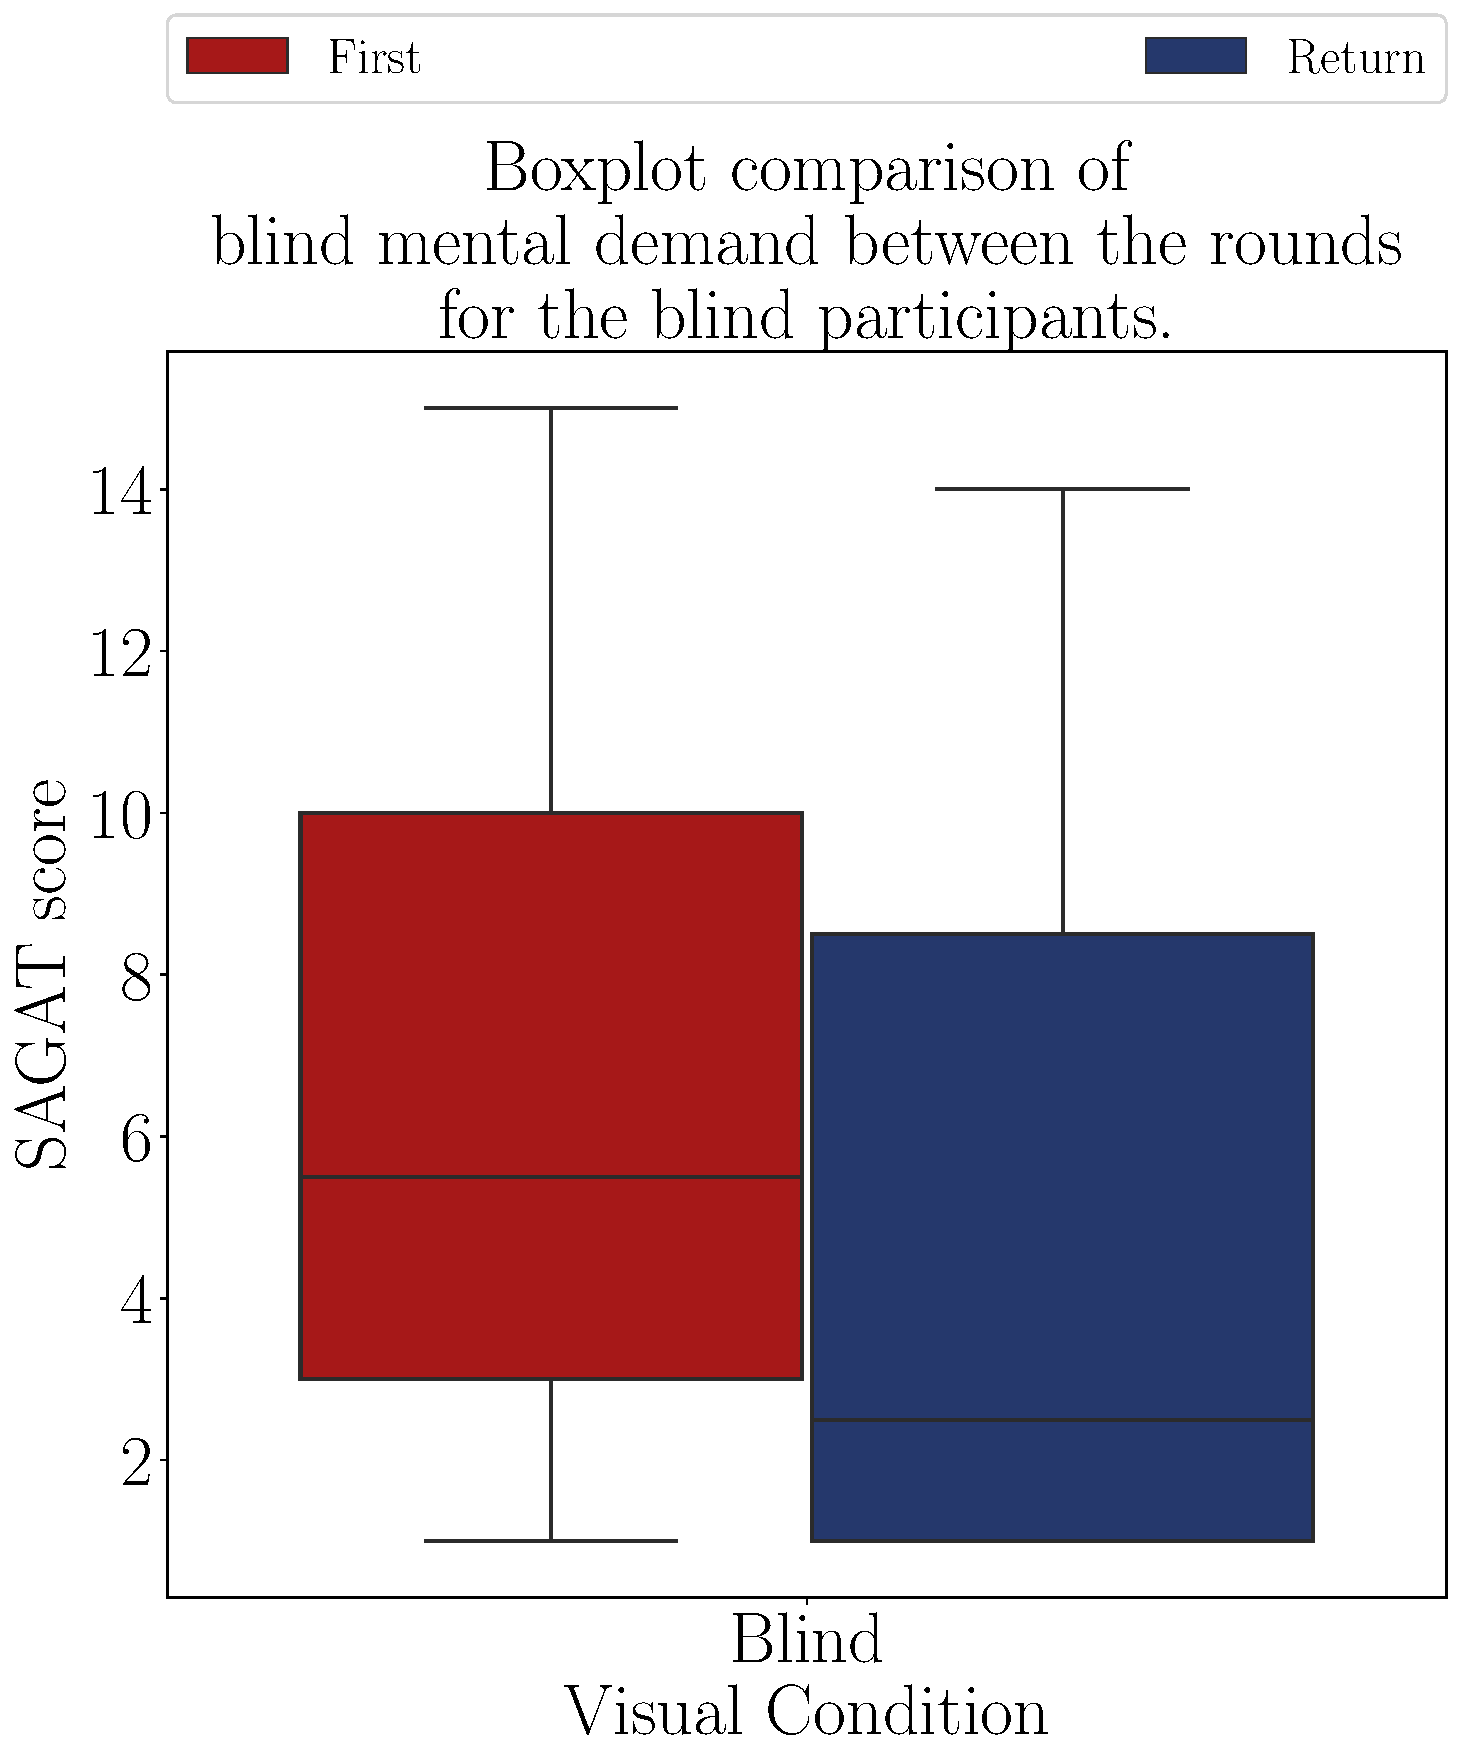
\includegraphics[width = 0.75\linewidth]{3 - Resultados/Figuras/boxplot_md_blind_rounds.pdf}
    \caption{Boxplot of the mental demand of the blind participants grouped by the rounds.}
    \label{fig:boxplot_md_blind_rounds}
\end{figure}

The results of ANOVA are presented in Table \ref{tab:blocanova_md_avg_two_way_blind}. A p-value of 0.05 is commonly adopted as a threshold to confirm the hypothesis. According to this criterion, neither method or round have a significant influence on the mental demand.


\begin{table}[!htb]
\centering
\caption{ANOVA p-value for mental demand -- blind participants}
\label{tab:blocanova_md_avg_two_way_blind}
\begin{tabular}{ll}
\toprule
          Source & P-Value \\
\midrule
    \    Methods &   0.170 \\
     \    Rounds &   0.075 \\
\    Interaction &   0.993 \\
\bottomrule
\end{tabular}
\end{table}



\paragraph*{Analysis of the NASA-TLX score}\mbox{}\\

Figure \ref{fig:boxplot_nasa_blind_scene} presents the boxplot with the NASA-TLX global score grouped by the methods. Similar to what happened for the "mental demand", it is possible to split the methods into two different groups: base and audio, which require a lower level of workload, and another group, which requires a higher level. Figure \ref{fig:boxplot_nasa_blind_rounds} presents a boxplot with the NASA-TLX global score grouped by the rounds, showing that the two groups are still different. 

\begin{figure}[!htb]
    \centering
    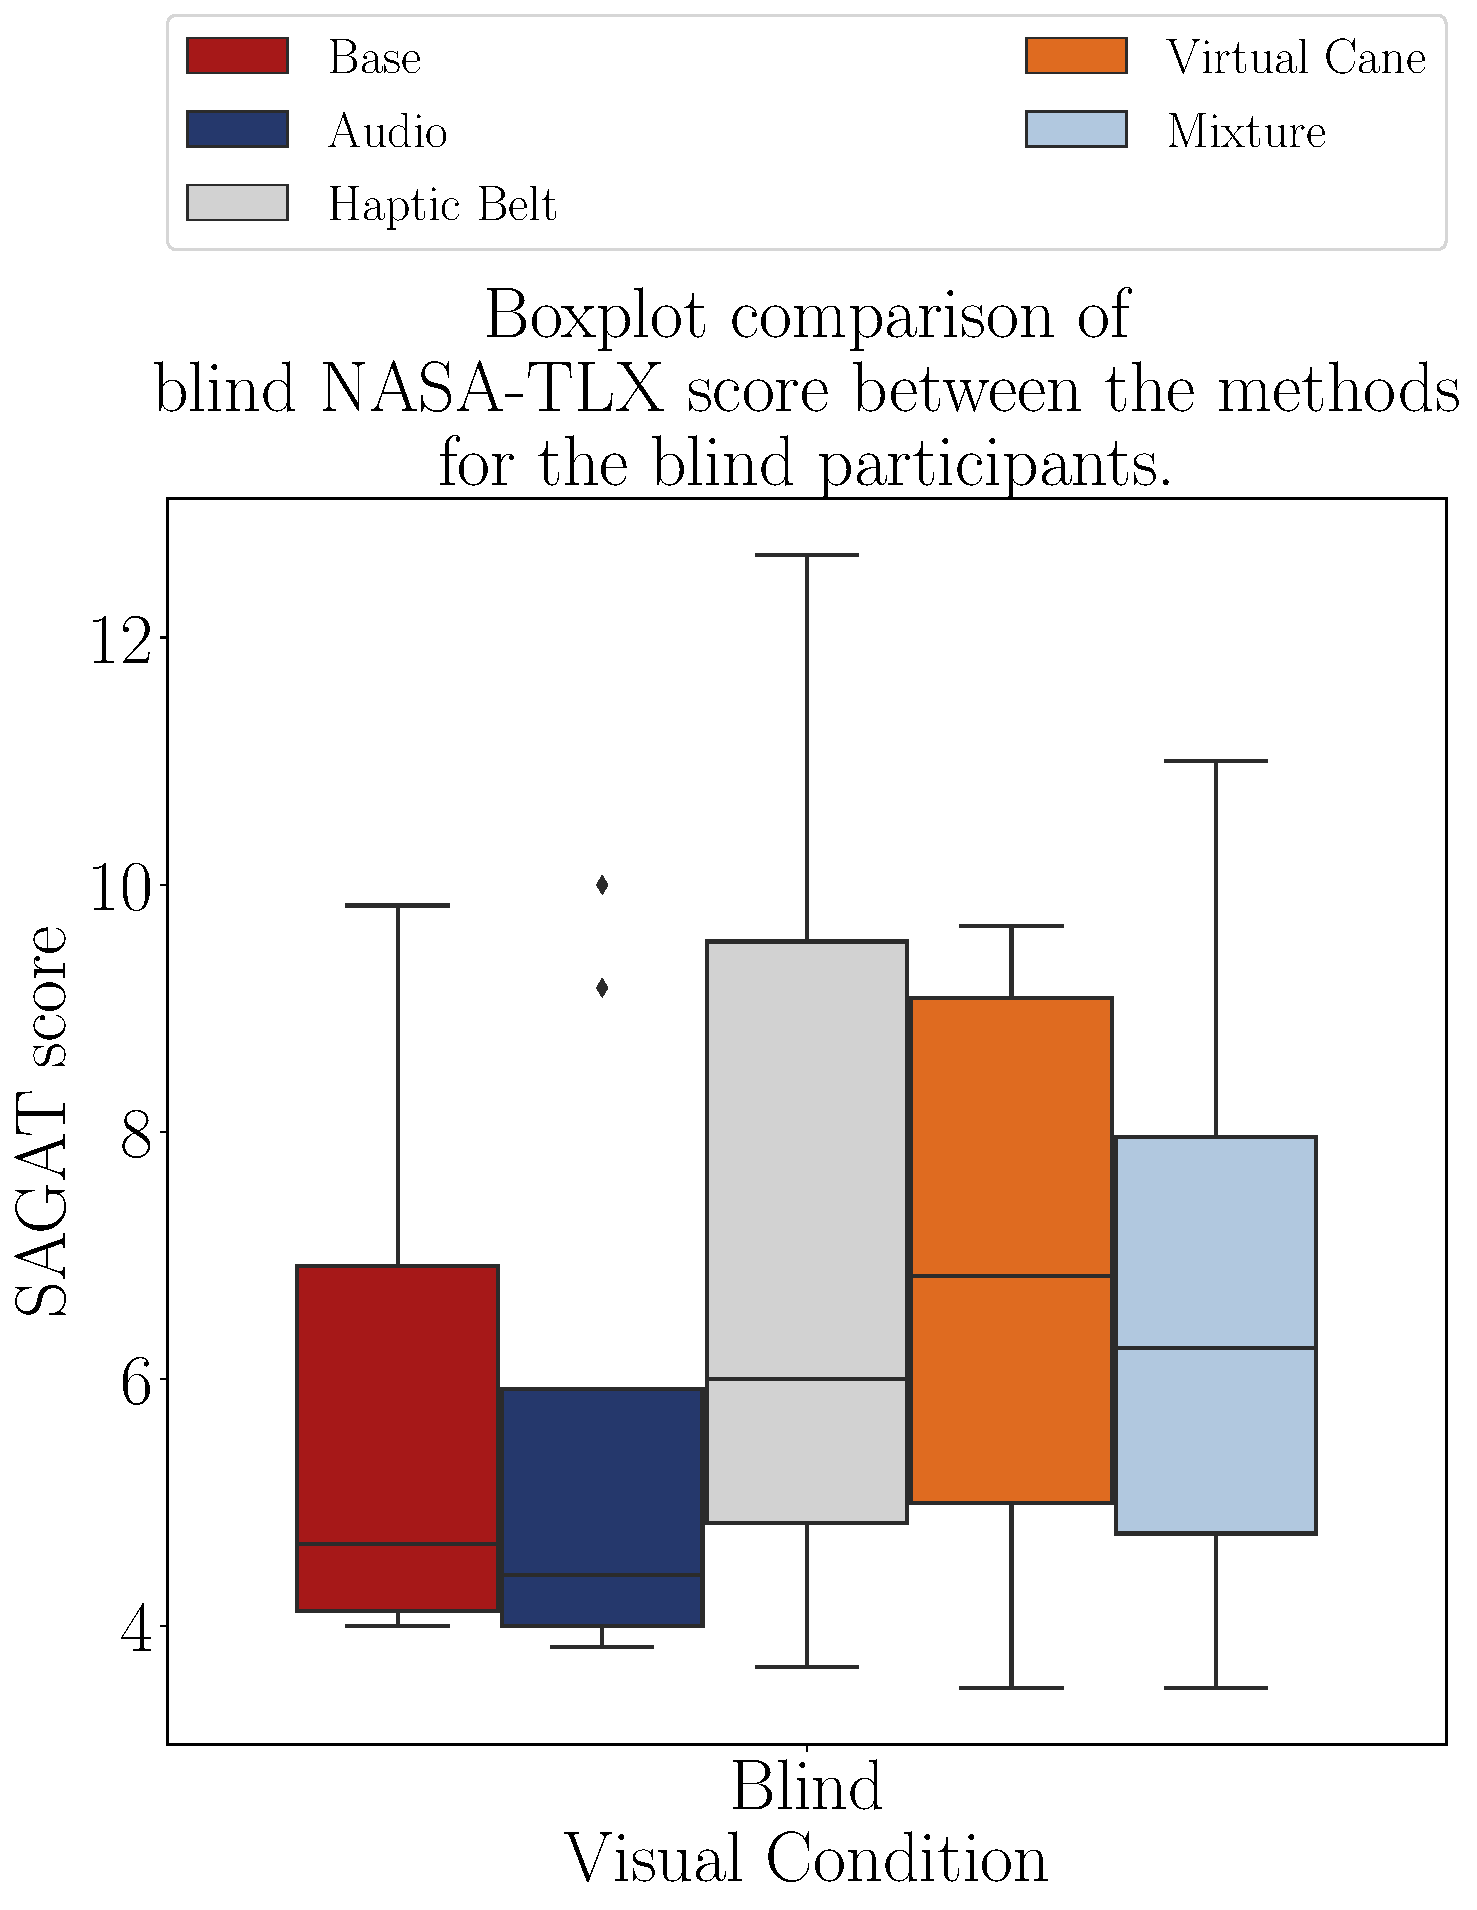
\includegraphics[width = 0.75\linewidth]{3 - Resultados/Figuras/boxplot_nasa_blind_scene.pdf}
    \caption{Boxplot of the mental demand of the blind participants grouped by the methods.}
    \label{fig:boxplot_nasa_blind_scene}
\end{figure}    
\begin{figure}[!htb]
    \centering
    %\vspace{3ex}
    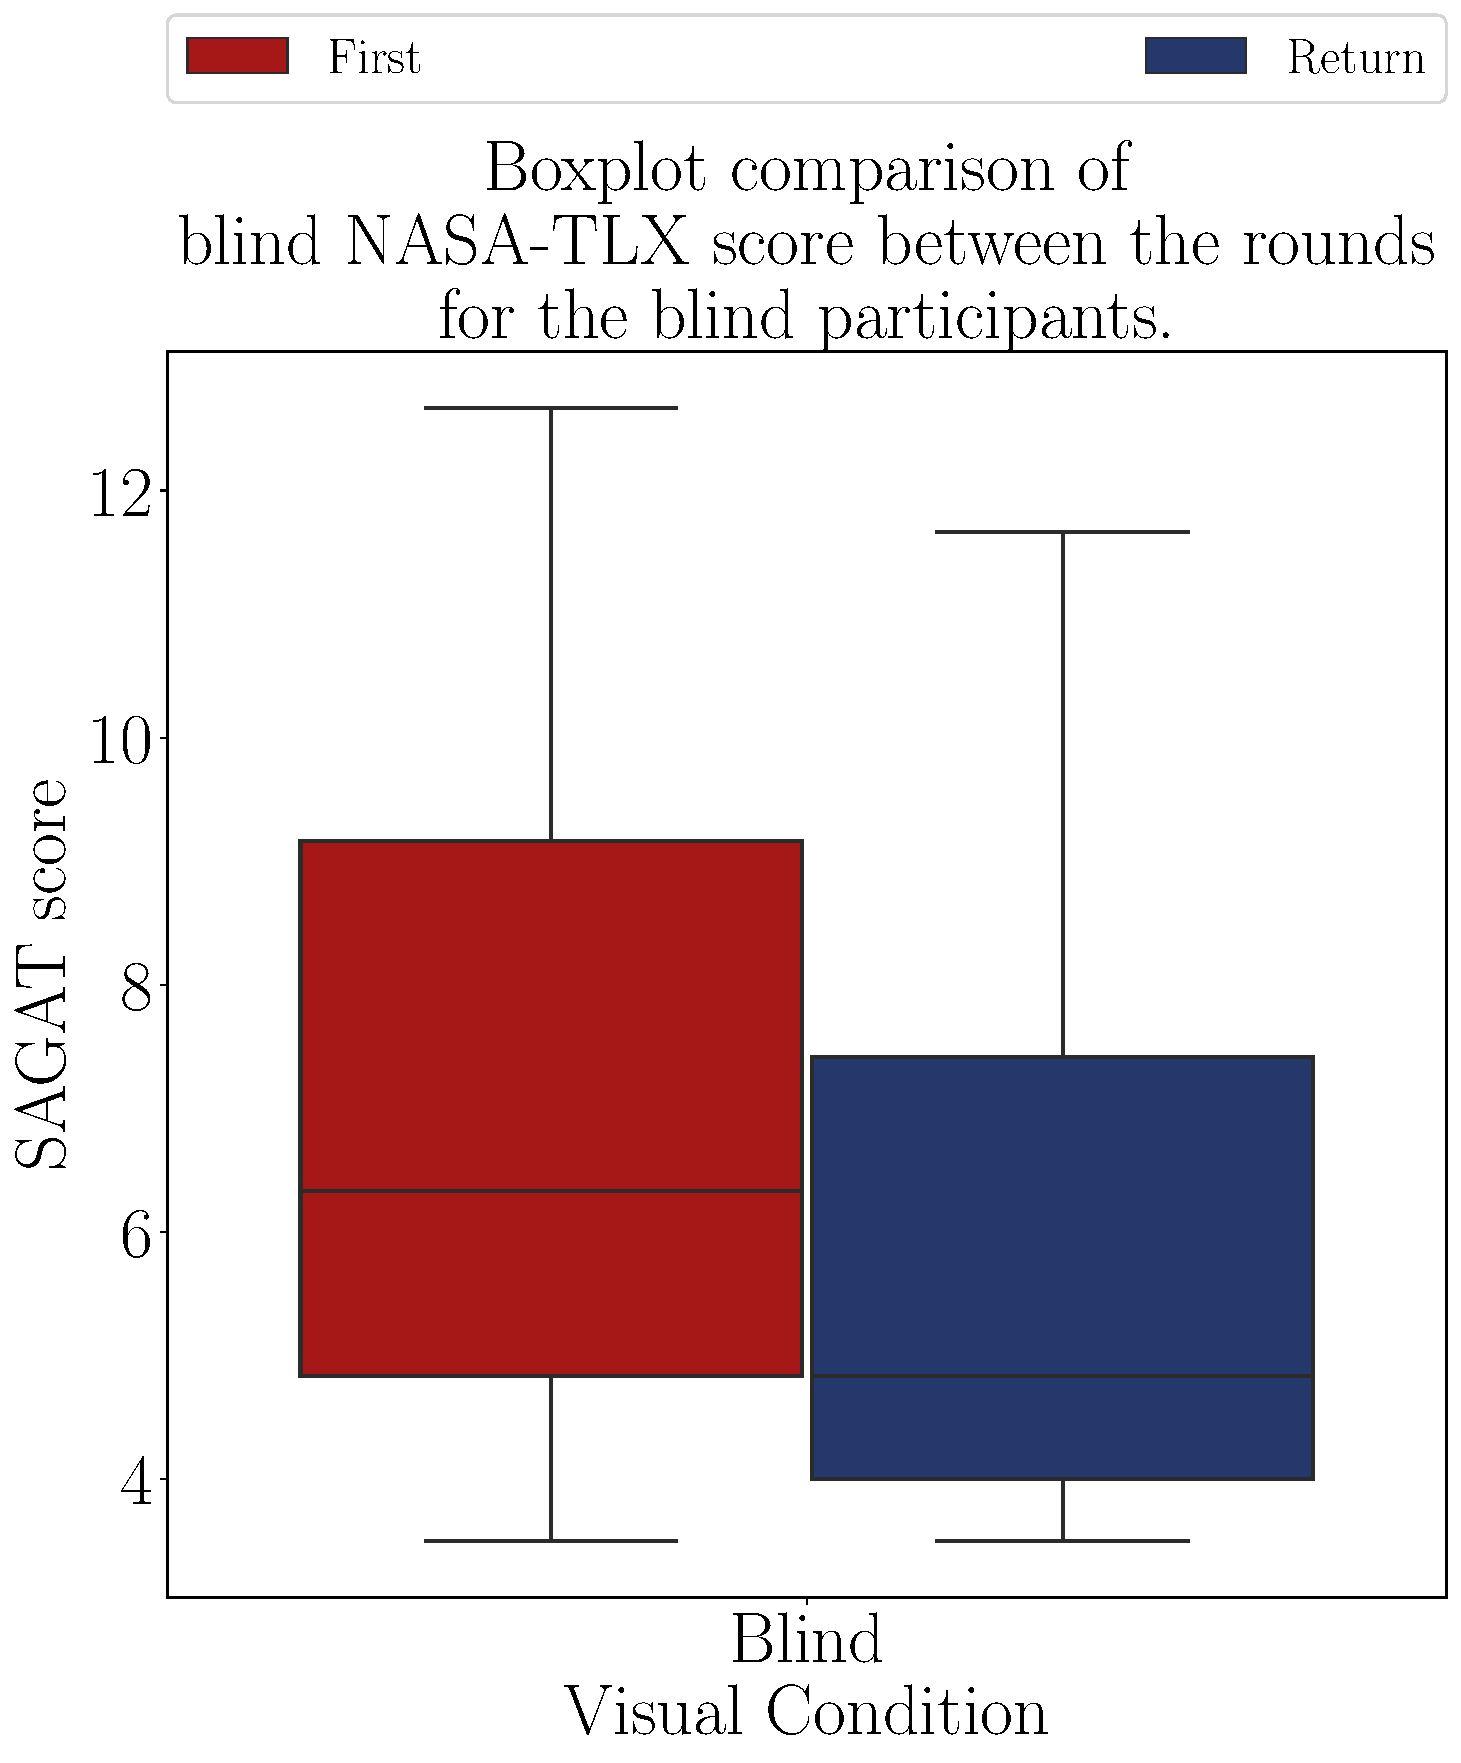
\includegraphics[width = 0.75\linewidth]{3 - Resultados/Figuras/boxplot_nasa_blind_rounds.pdf}
    \caption{Boxplot of the mental demand of the blind participants grouped by the rounds.}
    \label{fig:boxplot_nasa_blind_rounds}
\end{figure}

The sample residuals are not homogeneous meaning that the participants have different variability among them and that impacts the ANOVA.

Table \ref{tab:blocanova_nasa_avg_two_way_blind} brings the p-value resulting from ANOVA. In this case, both the methods and the rounds were appointed as significant variables that influence the mean value of the NASA-TLX global score. 


\begin{table}[!htb]
\centering
\caption{Anova p-value for the NASA-TLX score -- blinded users.}
\label{tab:blocanova_nasa_avg_two_way_blind}
\begin{tabular}{lrrrrl}
\toprule
          Source & P-Value \\
\midrule
    \    Methods & 0.029** \\
     \    Rounds & 0.022** \\
\    Interaction &   0.814 \\
\bottomrule
\end{tabular}
\end{table}



Finally a pairwise Fisher LSD test comparing each pair of guidance methods. The results show that only audio is similar to the base. All the other methods are different from each other.
\subsubsection{Adapted SAGAT}
\label{subsubsec:results_adapted_sagat_1}

For each question of the SAGAT questionnaire, the participant could score 1 point or a fraction of it. The closer to the value 1, higher is the situation awareness of the user. 

Figure \ref{fig:boxplot_sagat_blind_scene} brings the boxplot of the SAGAT score grouped by the guidance methods. It shows that the methods can be divided into two groups. The first one is composed of base, haptic belt and the mixture. This group received scores higher than the second group, composed of audio and virtual cane. Figure \ref{fig:boxplot_sagat_blind_rounds} shows the boxplot of the data grouped by round and confirms the general improvement of situation awareness from the first to the return round. 

\begin{figure}[!htb]
    \centering
    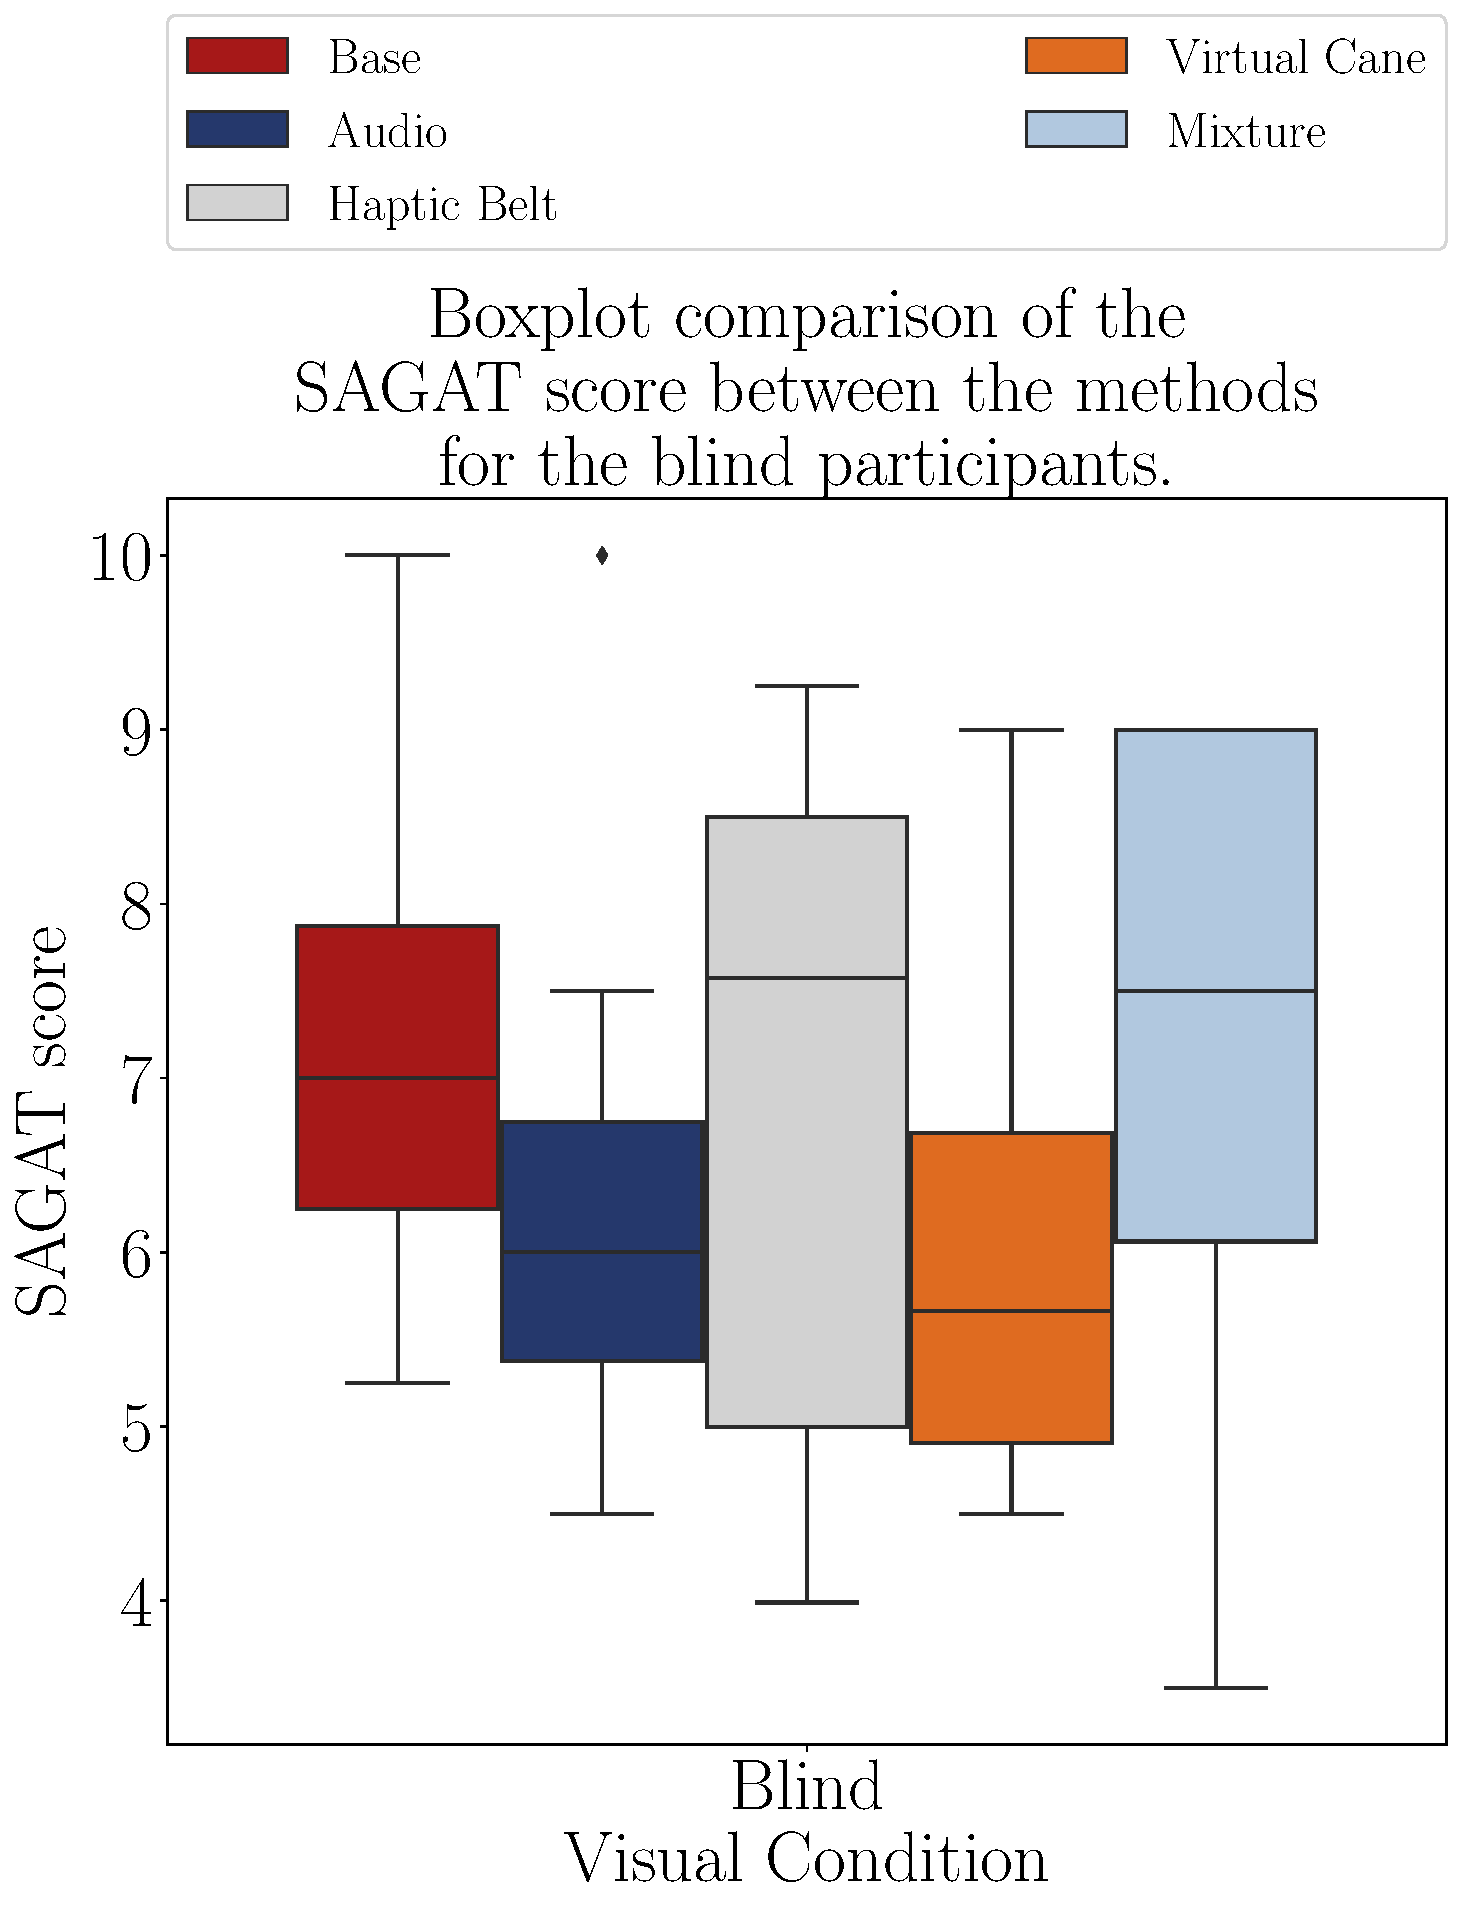
\includegraphics[width = 0.75\linewidth]{3 - Resultados/Figuras/boxplot_sagat_blind_scene.pdf}
    \caption{Boxplot of the SAGAT score of the blind participants grouped by the methods.}
    \label{fig:boxplot_sagat_blind_scene}
\end{figure}

\begin{figure}[!htb]
    \centering
    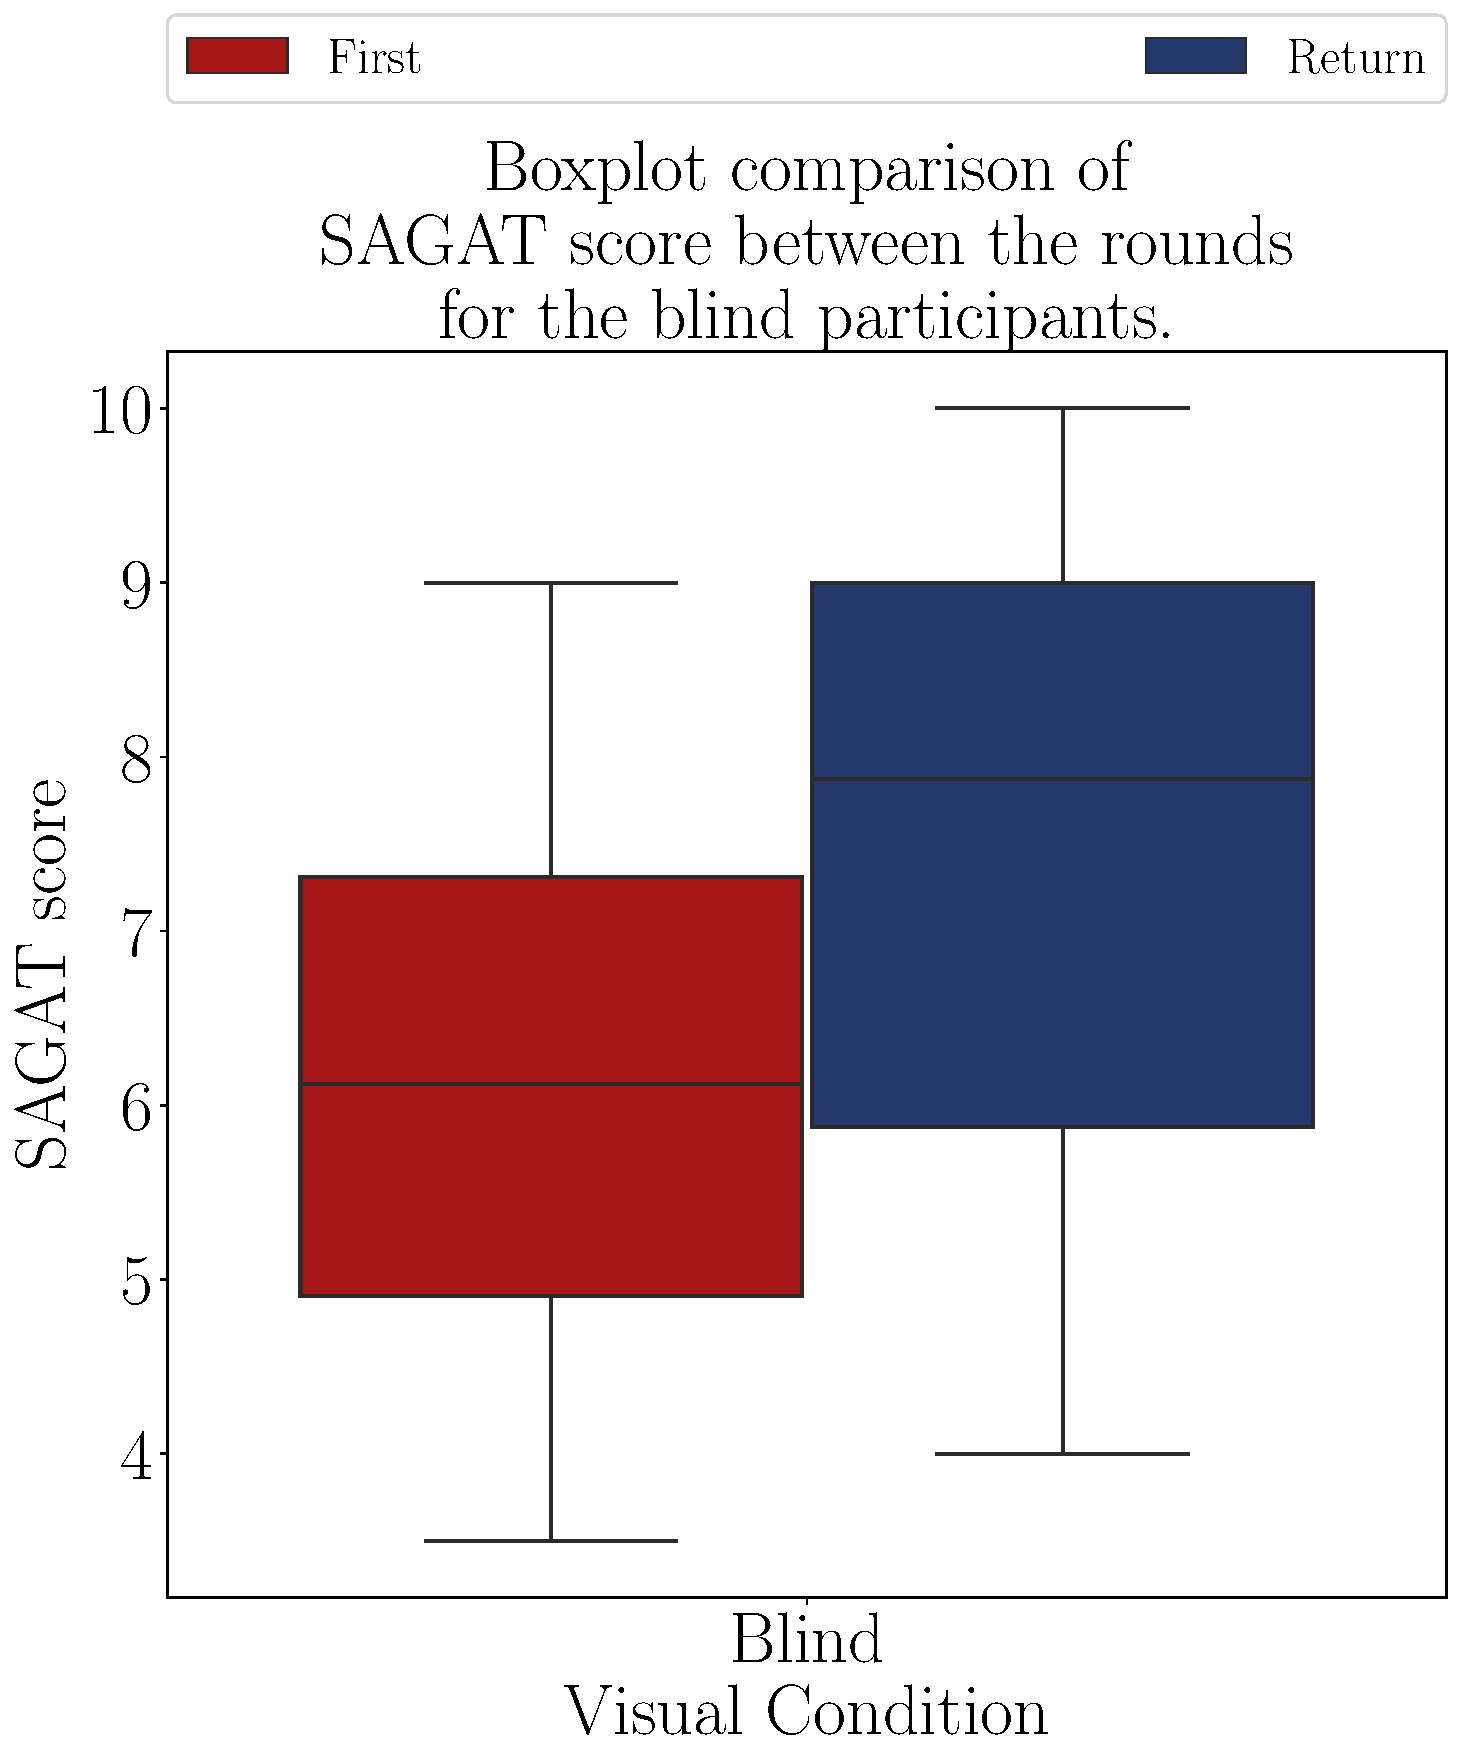
\includegraphics[width = 0.75\linewidth]{3 - Resultados/Figuras/boxplot_sagat_blind_rounds.pdf}
    \caption{Boxplot of the SAGAT score of the blind participants grouped by the rounds.}
    \label{fig:boxplot_sagat_blind_rounds}
\end{figure}

Table \ref{tab:blocanova_sagat_avg_two_way_blind} shows the ANOVA test p-value of the SAGAT score. It indicates that the round is a significant variable that influences the value of the SAGAT score. The same cannot be said for the method, which has no significant influence.


\begin{table}[!htb]
\centering
\caption{Anova p-value for the SAGAT score on each method for blinded users.}
\label{tab:blocanova_sagat_avg_two_way_blind}
\begin{tabular}{lrrrrr}
\toprule
          Source & P-Value \\
\midrule
    \    Methods &   0.277 \\
     \    Rounds & 0.002** \\
\    Interaction &   0.834 \\
\bottomrule
\end{tabular}
\end{table}


\subsubsection{Guidance method's questionnaire.}
\label{subsubsec:results_questionnaires}

The data from the questionnaire for evaluating the user experience with each guidance method is also analysed. The higher the score, the more satisfied the user is with the method. It is essential to observe that this analysis does not include the base method as the questions are specific about each method and the base may vary among the participants. Also, there is no distinction between first and return rounds. Each questionnaire is answered only once for each method.
Figure \ref{fig:boxplot_quest_blind_scene} brings the questionnaire boxplot, which clearly shows the difference between two groups: haptic belt and virtual cane, and audio and mixture. 

\begin{figure}[!htb]
    \centering
    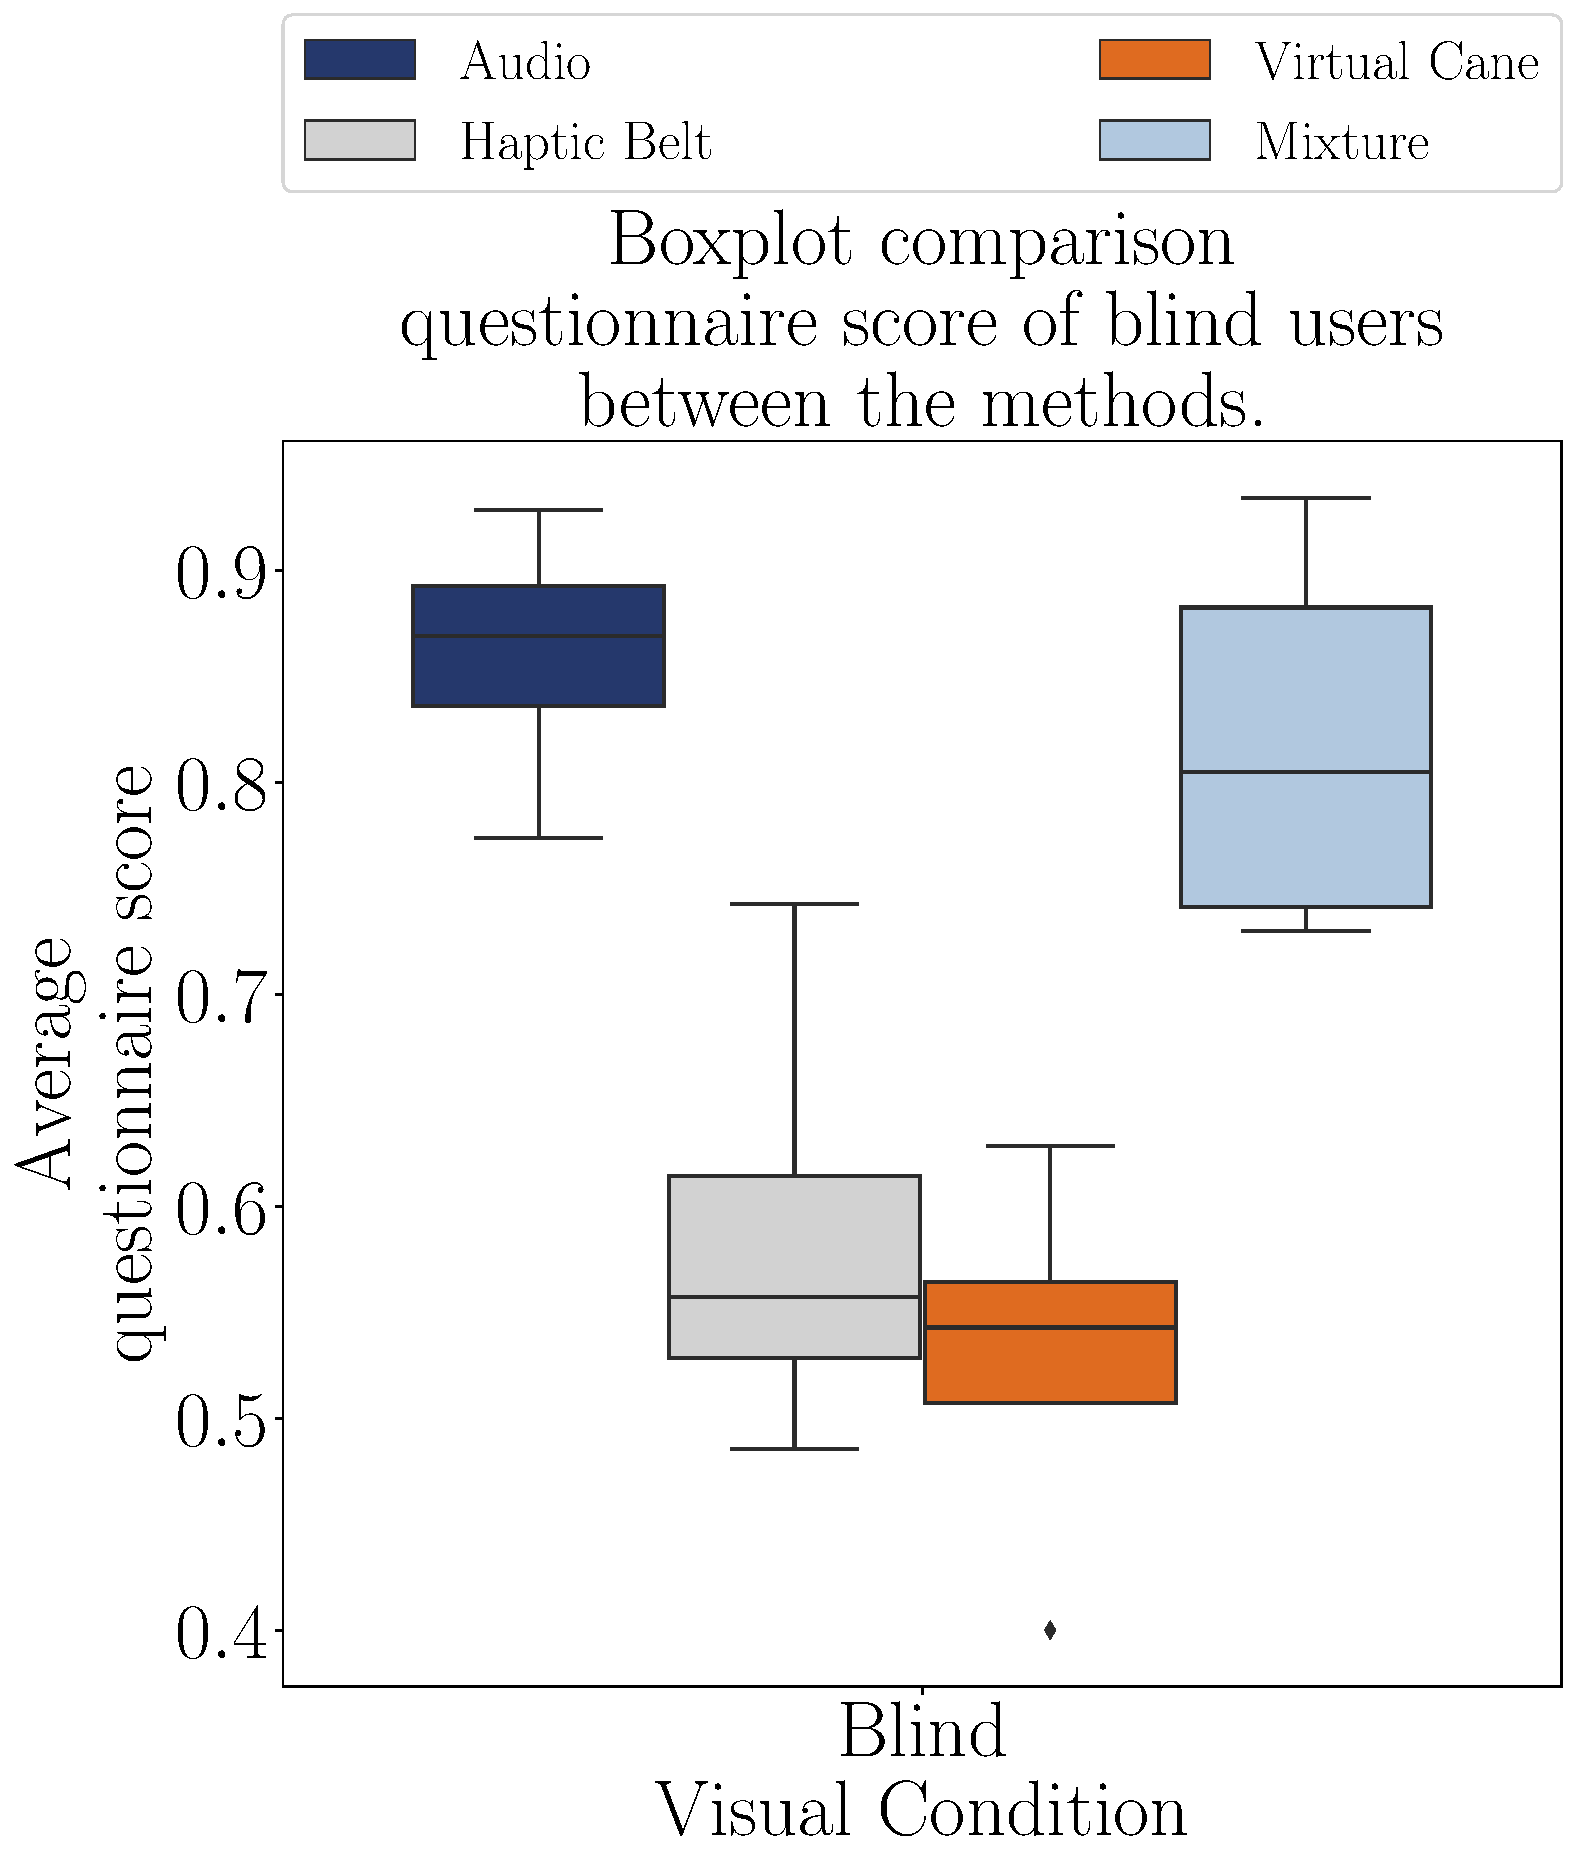
\includegraphics[width = 0.75\linewidth]{3 - Resultados/Figuras/boxplot_questionnaire_scene_blind.pdf}
    \caption{Boxplot of the questionaire score of the blind participants grouped by the methods.}
    \label{fig:boxplot_quest_blind_scene}
\end{figure}

The results of ANOVA are presented in Table  \ref{tab:blocanova_questionnaire_blind} and it shows that the method, with a p-value of 0.001, is indeed a significant variable that affects the user's satisfaction.


\begin{table}[!htb]
\centering
\caption{Anova p-value for the questionnaire score -- blinded users.}
\label{tab:blocanova_questionnaire_blind}
\begin{tabular}{lrrrrr}
\toprule
Source & P-Value \\
\midrule
Method & 0.001** \\
\bottomrule
\end{tabular}
\end{table}



In order to complement the ANOVA analysis, the pairwise comparison of the methods obtained from the Fisher LSD shows that audio and mixture are equivalent from the perspective of user satisfaction. All the other comparisons indicate there is a difference between the methods.

Additional to the scores, the participants also expressed their dissatisfaction with the answers to the open questions of the questionnaire, where they commented that the haptic belt and the virtual cane are confusing, are not precise enough, and are very different from what they are used to.

%\subsection{Physiological data}

%During the experiment, data from two physiological sensors were captured: ECG and GSR. As commonly found in the literature, these data are used to assess mental workload. The corresponding analysis is presented in this section.

\subsubsection{Electrocardiogram (ECG) data}
\label{subsubsec:results_ecg_1}

After the experiment, the ECG signal processing is organized in the following steps: 

\begin{itemize}
    \item Filtering and removing outliers. Since the participants moved during the whole experience, the sensors also captured some noise data.
    \item Normalization between -1 and 1;
    \item Peak detection and evaluation – if the results were not of good quality, the peak detection method's parameters were adjusted to improve it; 
    \item Calculation of BPM using Kubius HRV Standard;
    \item Calculation of SDNN using Kubius HRV Standard.
\end{itemize}

At the beginning of each experiment, a baseline was collected to establish a comparison between the relaxed state of the participant and the scenes' induced state. However, the results were not consistent.  During the experiment, it was expected that the heart rate would increase compared to the baseline because the participants were at rest. However, for most of the participants, it decreased, indicating a systematic problem may have occurred. Due to this fact, the analysis is based only on absolute values.

\paragraph*{Analysis of the heartbeat frequency (BPM)}\mbox{}\\

Figures \ref{fig:boxplot_ecg_bpm_blind_scene} and \ref{fig:boxplot_ecg_bpm_blind_rounds} brings the corresponding boxplot, grouped by method and round. In both cases, it is not possible to observe significant differences among the methods or rounds.

\begin{figure}[!htb]
    \centering
    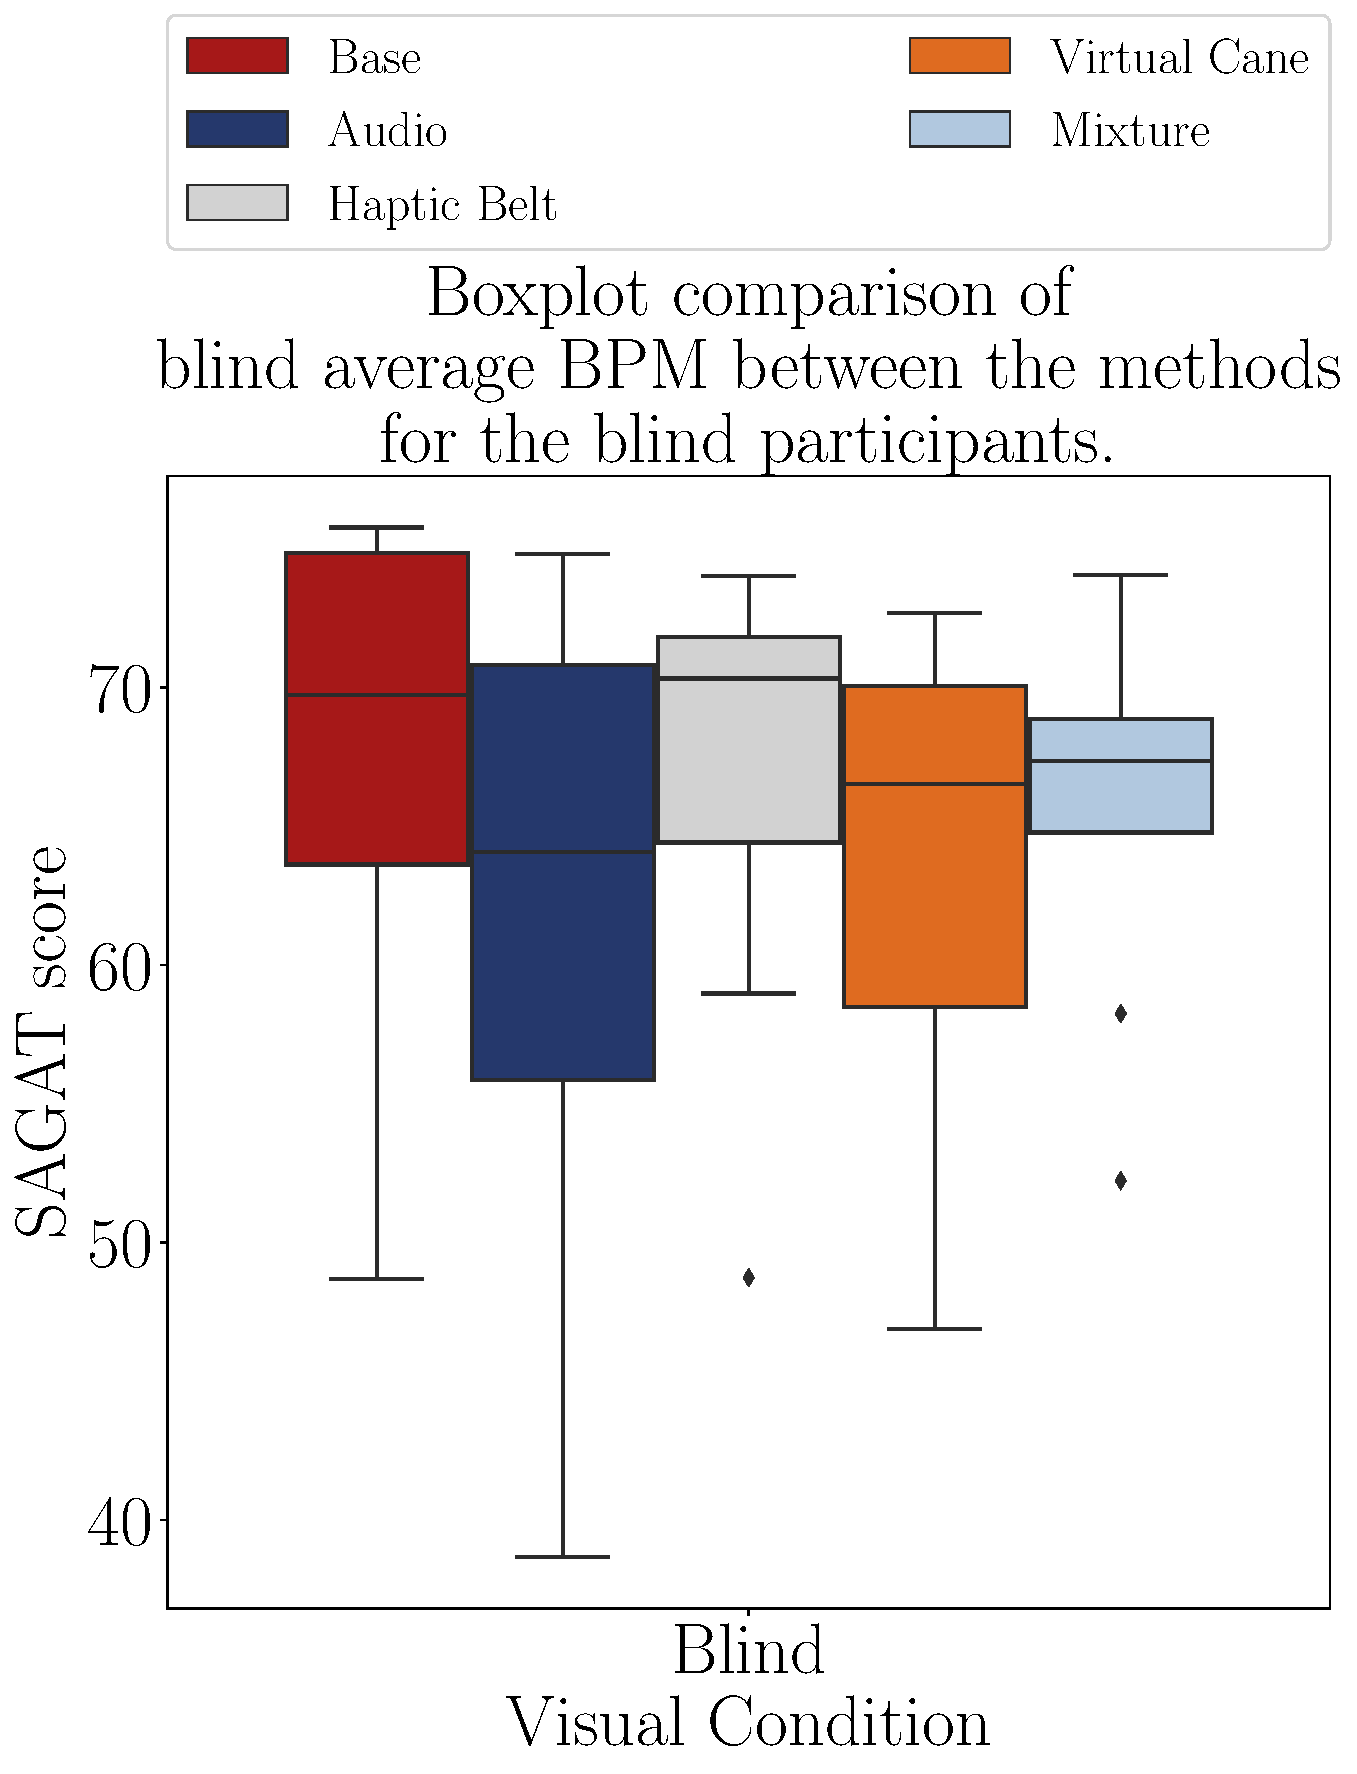
\includegraphics[width = 0.75\linewidth]{3 - Resultados/Figuras/boxplot_ecg_bpm_blind_scene.pdf}
    \caption{Boxplot of the BPM of the blind participants grouped by the methods.}
    \label{fig:boxplot_ecg_bpm_blind_scene}
\end{figure}

\begin{figure}[!htb]
    \centering
    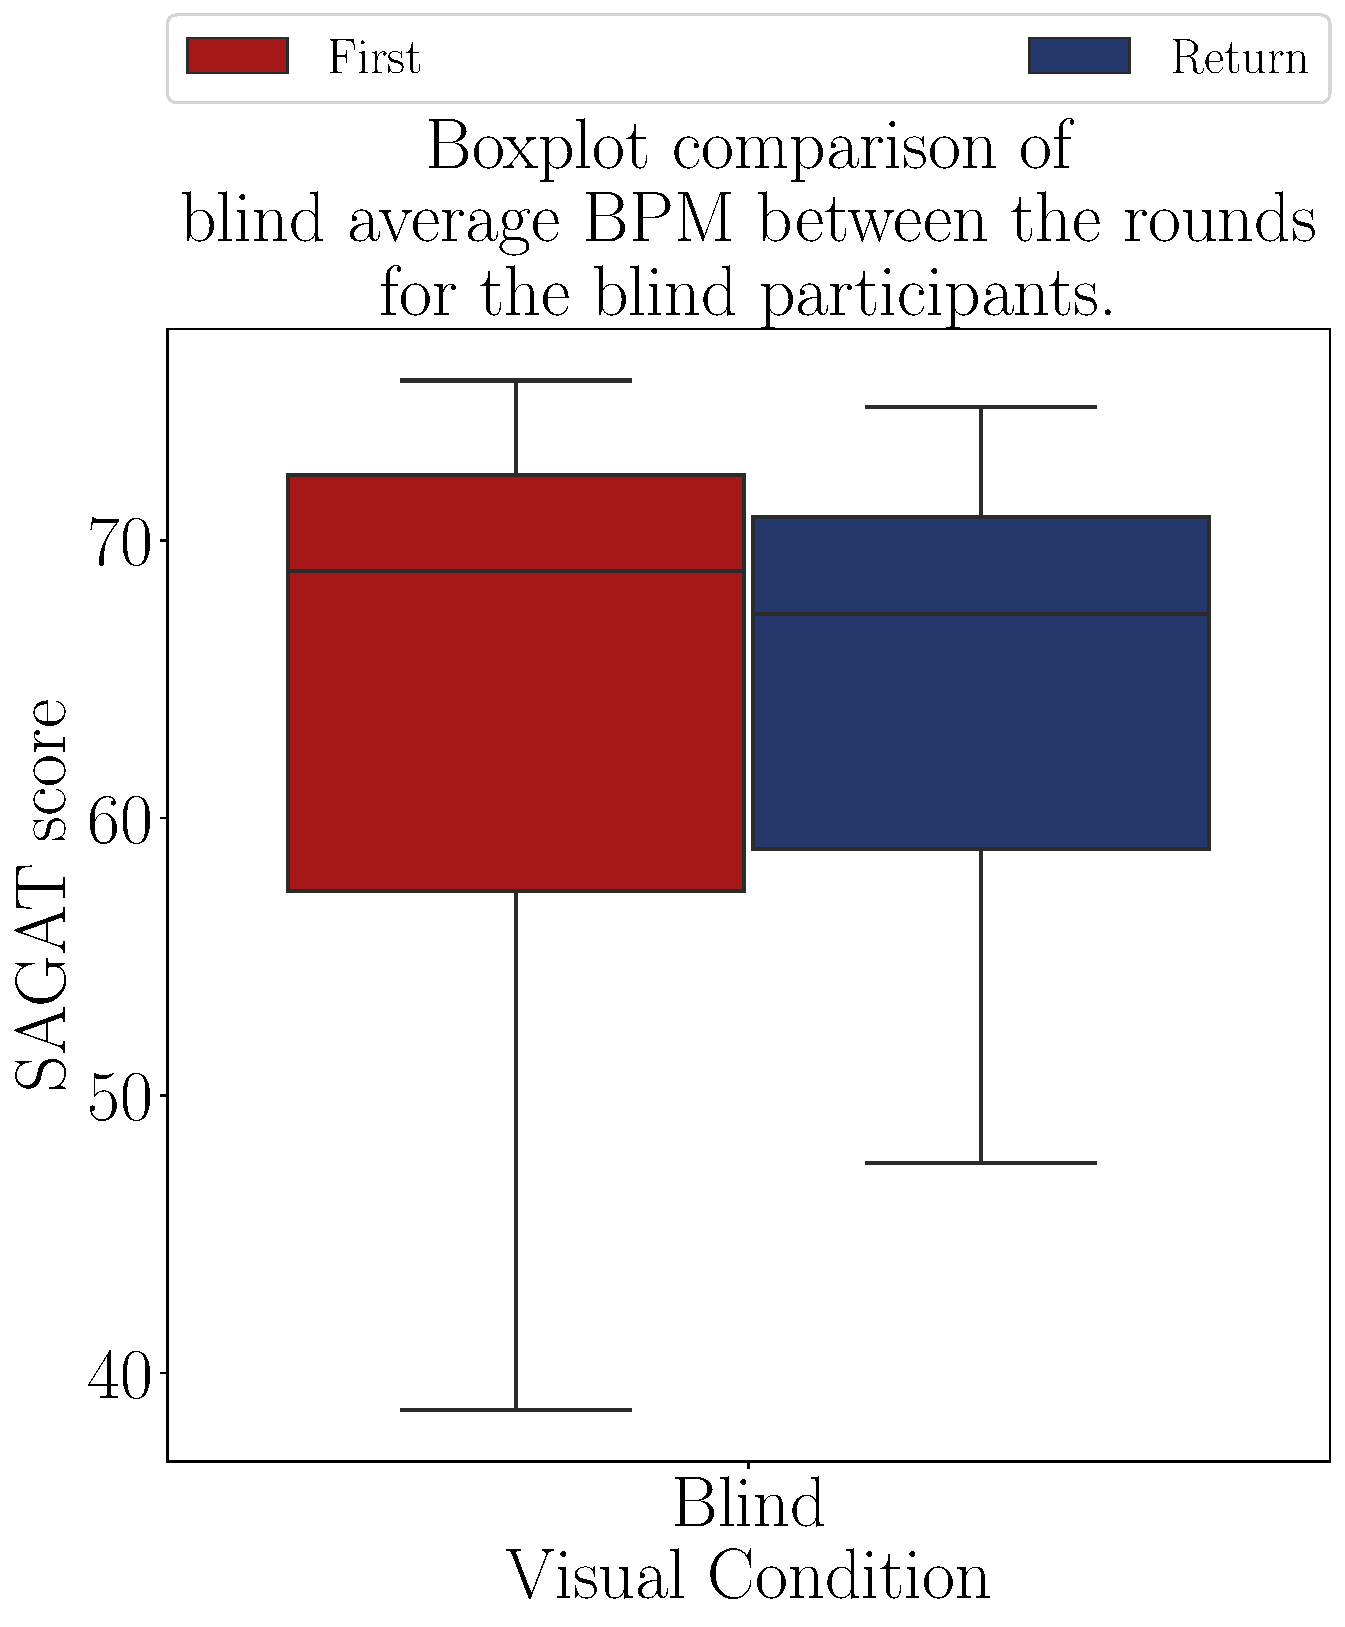
\includegraphics[width = 0.75\linewidth]{3 - Resultados/Figuras/boxplot_ecg_bpm_blind_rounds.pdf}
    \caption{Boxplot of the BPM of the blind participants grouped by the rounds.}
    \label{fig:boxplot_ecg_bpm_blind_rounds}
\end{figure}

The participants do not have a similar variance, which jeopardize the results of ANOVA. Considering this limitation, Table \ref{tab:blocanova_bpm_two_way_blind} brings the p-value obtained by ANOVA, which confirmed the previous analysis, as it does not indicate a significant influence of either the guidance methods or the rounds in the participants' heart rate. 


\begin{table}[!htb]
\centering
\caption{Anova p-value for the BPM -- blinded users.}
\label{tab:blocanova_bpm_two_way_blind}
\begin{tabular}{lrrrrr}
\toprule
          Source & P-Value \\
\midrule
    \    Methods &   0.100 \\
     \    Rounds &   0.371 \\
\    Interaction &   0.894 \\
\bottomrule
\end{tabular}
\end{table}



%%%%%%%%%%%%%%%%%%%%%%%%%%%%%%%%%%%%%%%%%%%%%%%%%%%%%%%%%%%%%%%%%%%%%%%%%%%%
%%%%%%%%%%%%%%%%%%%%%%%%%%%%%%%%%%%%%%%%%%%%%%%%%%%%%%%%%%%%%%%%%%%%%%%%%%%%
%%%%%%%%%%%%%%%%%%%%%%%%%%%%%%%%%%%%%%%%%%%%%%%%%%%%%%%%%%%%%%%%%%%%%%%%%%%%
%%%%%%%%%%%%%%%%%%%%%%%%%%%%%%%%%%%%%%%%%%%%%%%%%%%%%%%%%%%%%%%%%%%%%%%%%%%%

\paragraph*{Analysis of the heartbeat variance (SDNN)}\mbox{}\\

Figure \ref{fig:boxplot_ecg_sdnn_blind_scene} and Figure \ref{fig:boxplot_ecg_sdnn_blind_rounds} bring the SDNN barplot grouped by the methods and the rounds. There is a slight tendency among the participants to increase the heartbeat in the return round.

\begin{figure}[!htb]
    \centering
    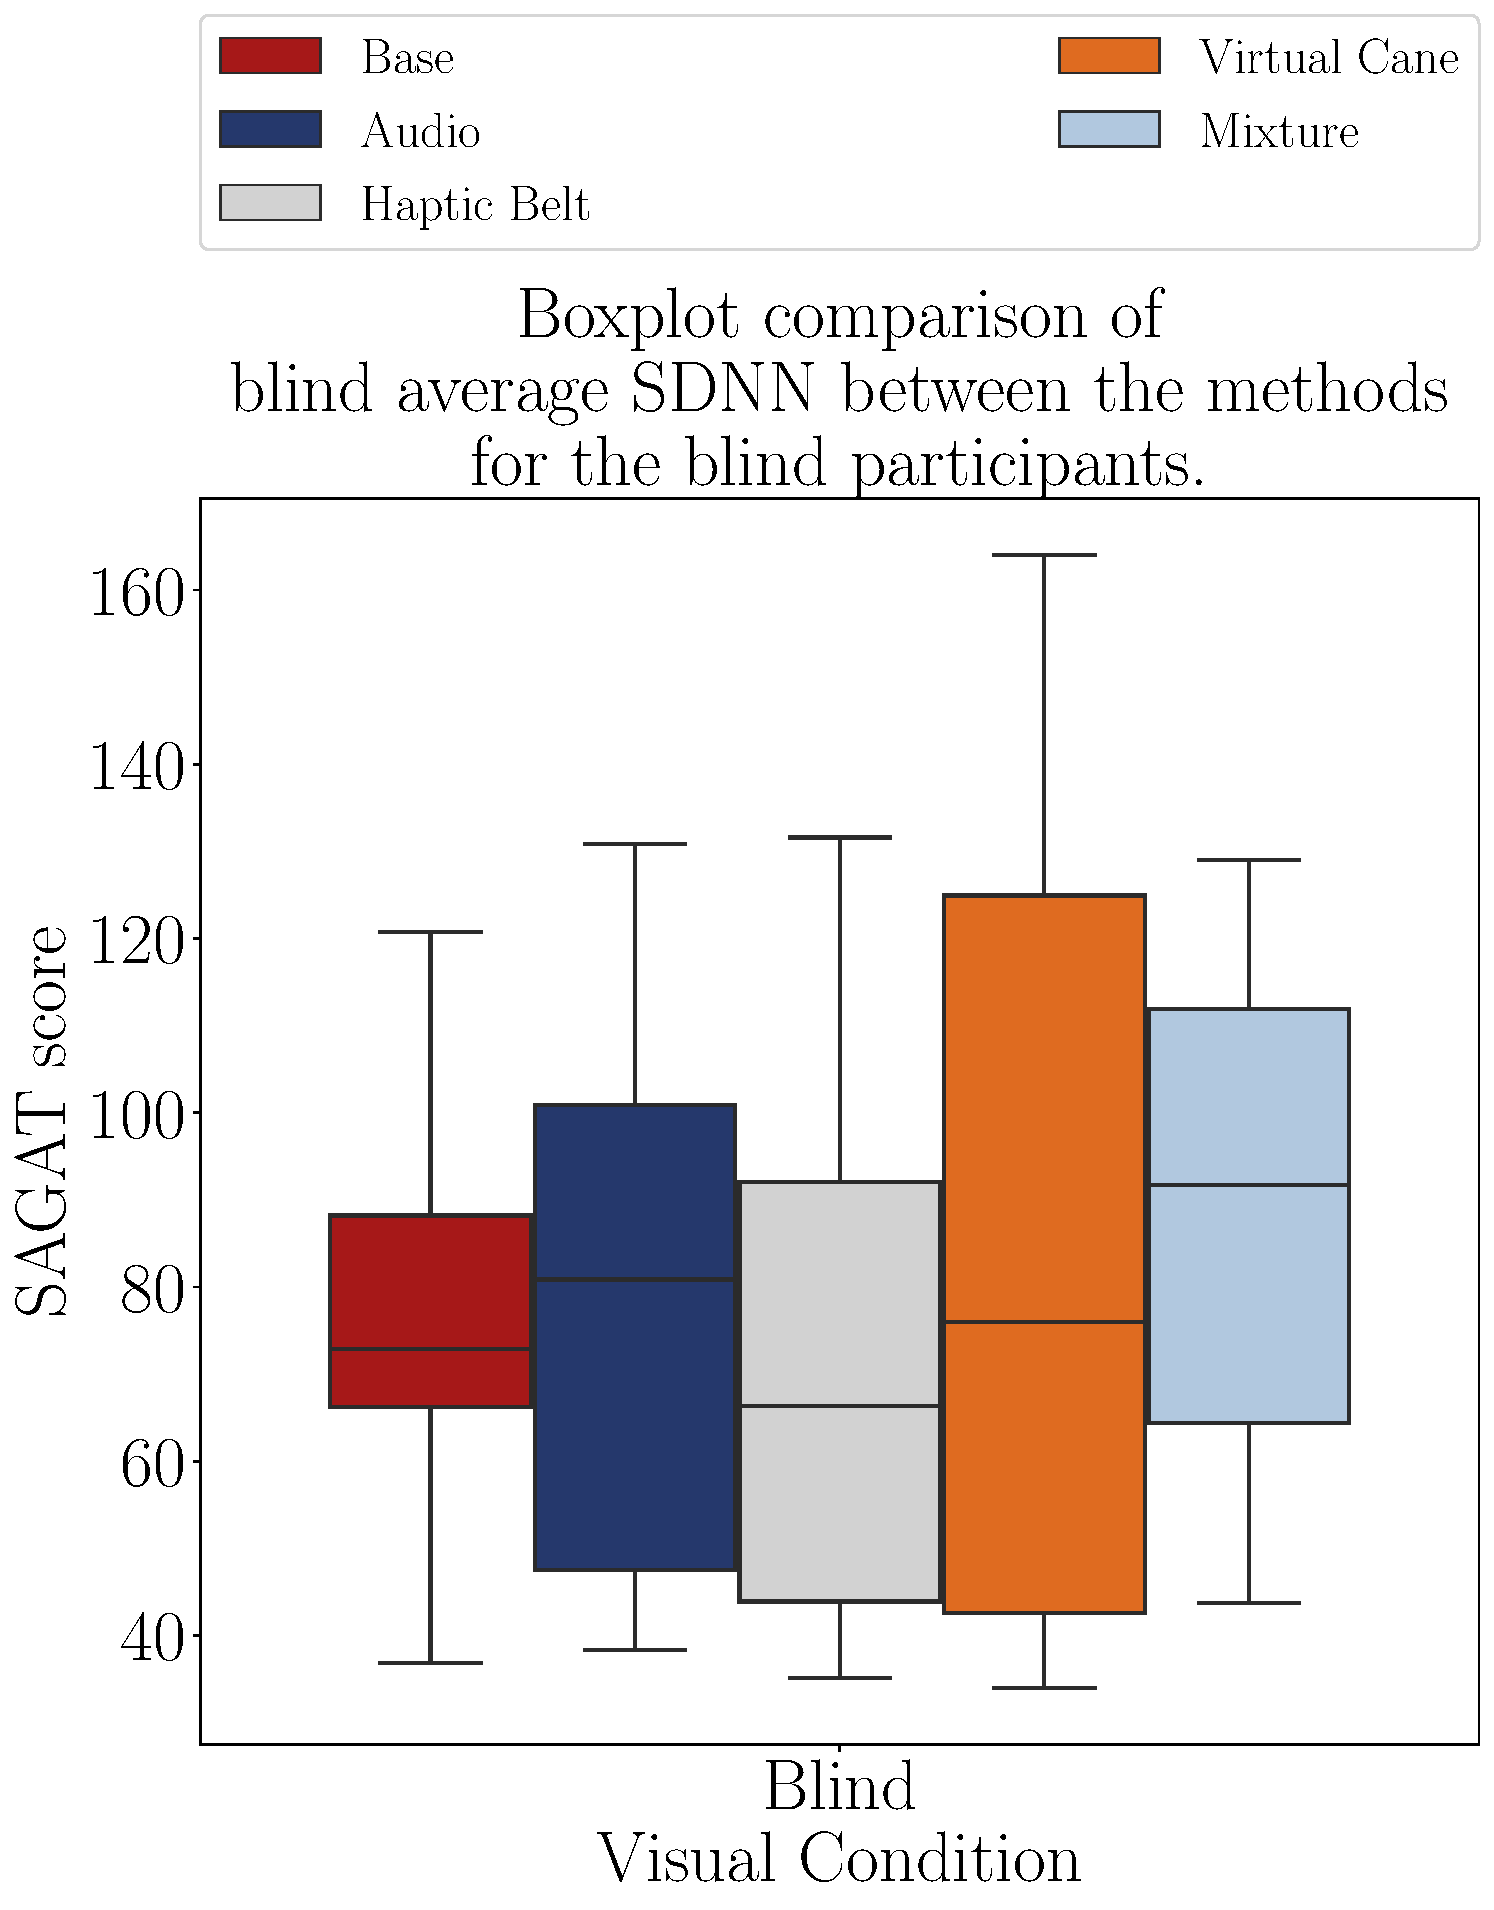
\includegraphics[width = 0.75\linewidth]{3 - Resultados/Figuras/boxplot_ecg_sdnn_blind_scene.pdf}
    \caption{Boxplot of the SDNN of the blind participants grouped by the methods.}
    \label{fig:boxplot_ecg_sdnn_blind_scene}
\end{figure}
\begin{figure}[!htb]
    \centering
    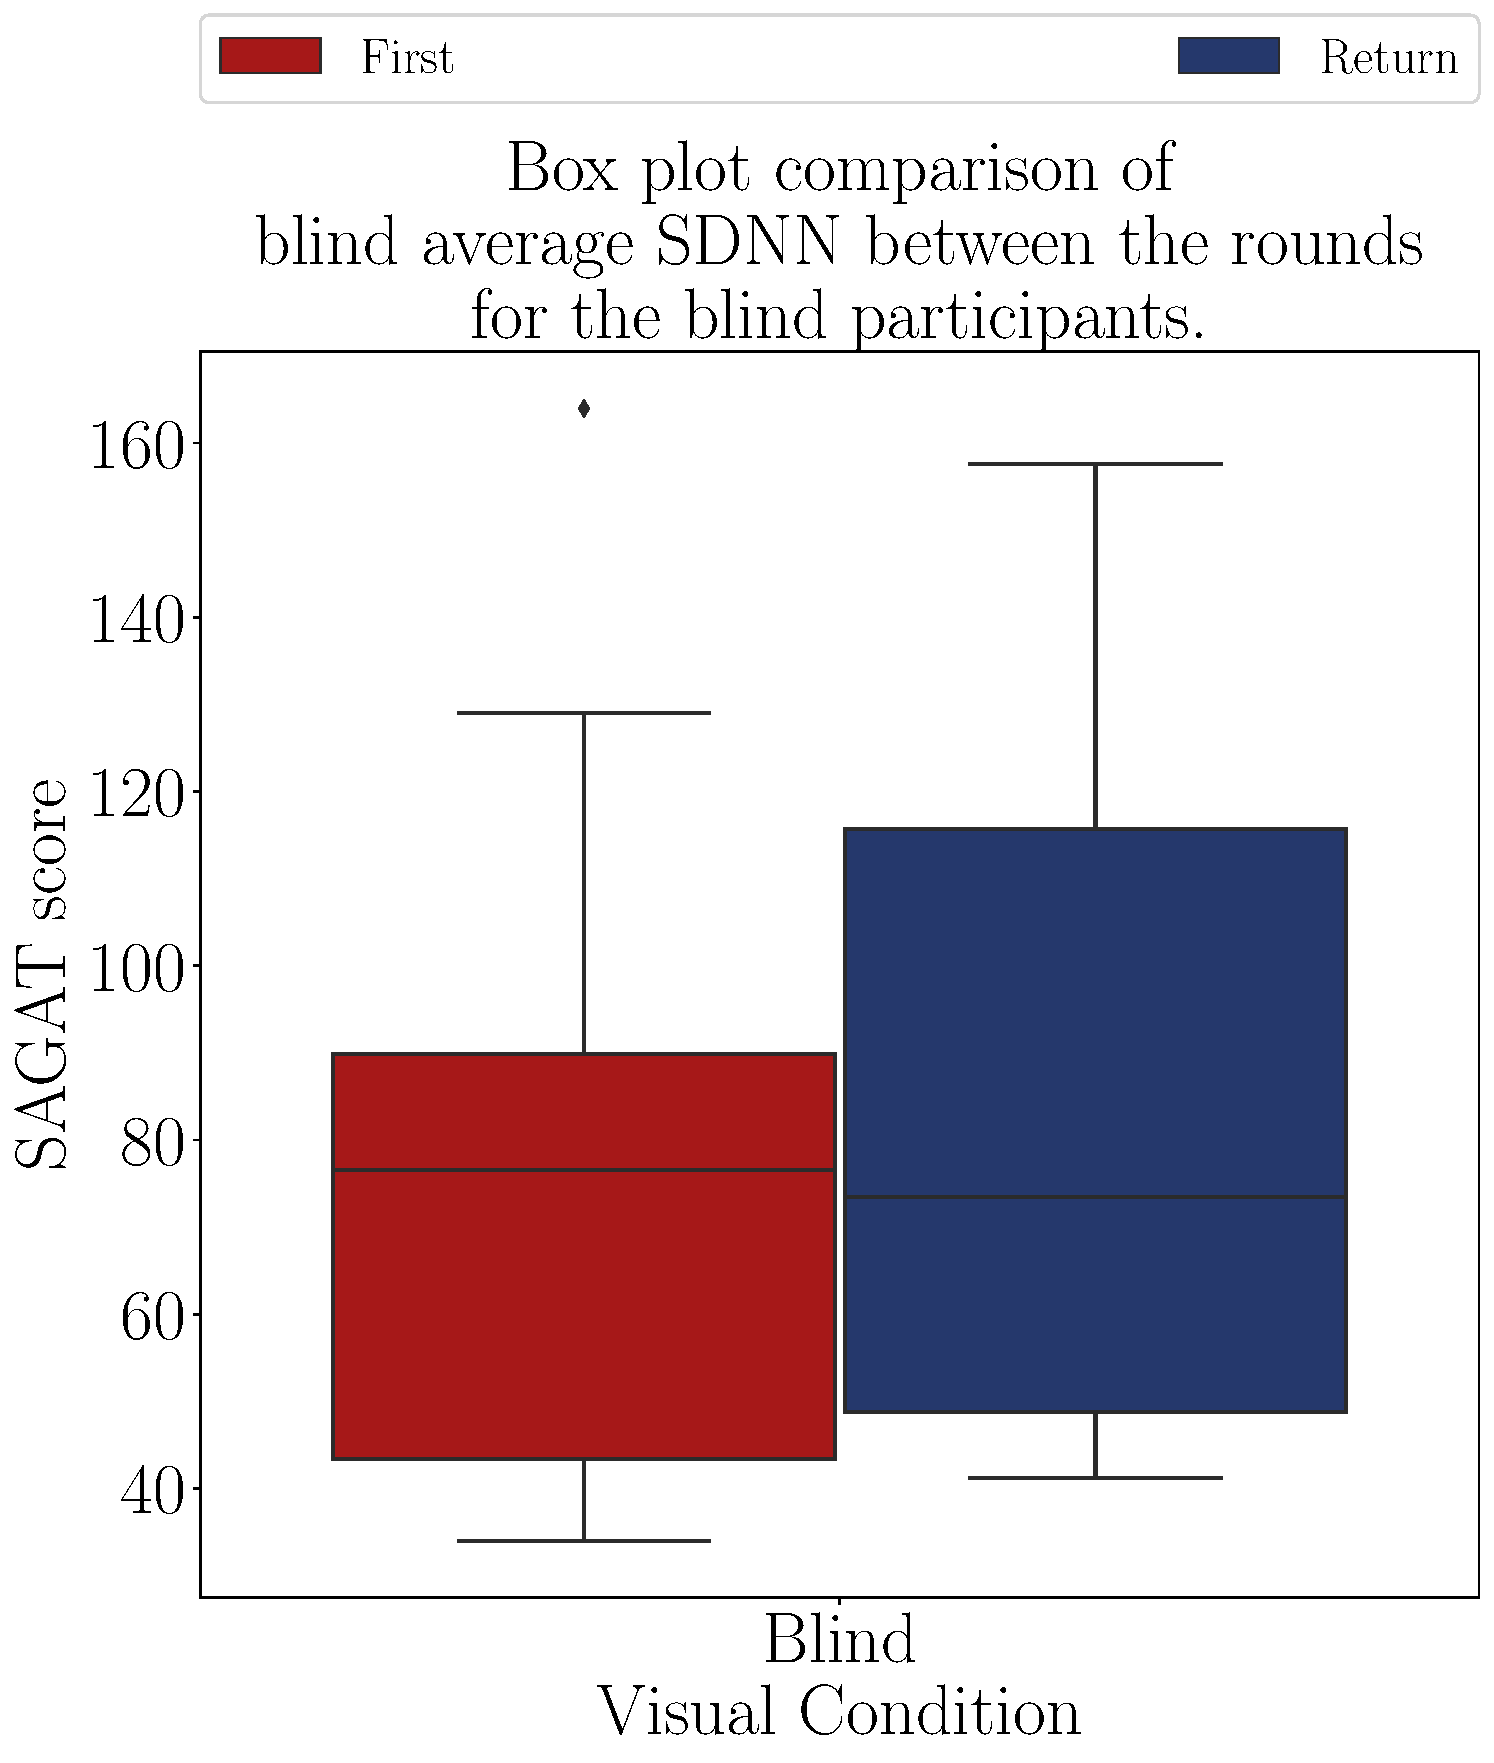
\includegraphics[width = 0.75\linewidth]{3 - Resultados/Figuras/boxplot_ecg_sdnn_blind_rounds.pdf}
    \caption{Boxplot of the SDNN of the blind participants grouped by the rounds.}
    \label{fig:boxplot_ecg_sdnn_blind_rounds}
\end{figure}

The ANOVA results are presented in Table \ref{tab:blocdanova_sdnn_two_way_blind} and do not confirm any influence of the methods nor the rounds on the ECG heart rate variance.


\begin{table}[H]
\centering
\caption{Anova p-value for the average SDNN -- blinded users.}
\label{tab:blocdanova_sdnn_two_way_blind}
\begin{tabular}{lrrrrr}
\toprule
          Source & P-Value \\
\midrule
    \    Methods &   0.486 \\
     \    Rounds &   0.223 \\
\    Interaction &   0.473 \\
\bottomrule
\end{tabular}
\end{table}



\subsubsection{Galvanic skin response and temperature data;}
\label{subsubsec:results_gsr_temp_1}

The GSR analysis is based on the signal's average level. Each experiment's round is compared to the participant baseline collected before the experiment. The GSR sensor was worn on the left hand for right-handed participant and on the right hand for left-handed participants. One of the blind participants had the GSR sensor removed during the experiment because it was not appropriately fixed.

Figure \ref{fig:boxplot_gsr_avg_blind_scene} presents the boxplot of the percentual variation in the skin conductance for each method. The base method has the lowest variation among all methods. Also, the introduction of vibration increases the method variance. Figure \ref{fig:boxplot_gsr_avg_blind_rounds} presents the GSR grouped by the rounds. In this case, there is no apparent difference between the rounds.

\begin{figure}[!htb]
    \centering
    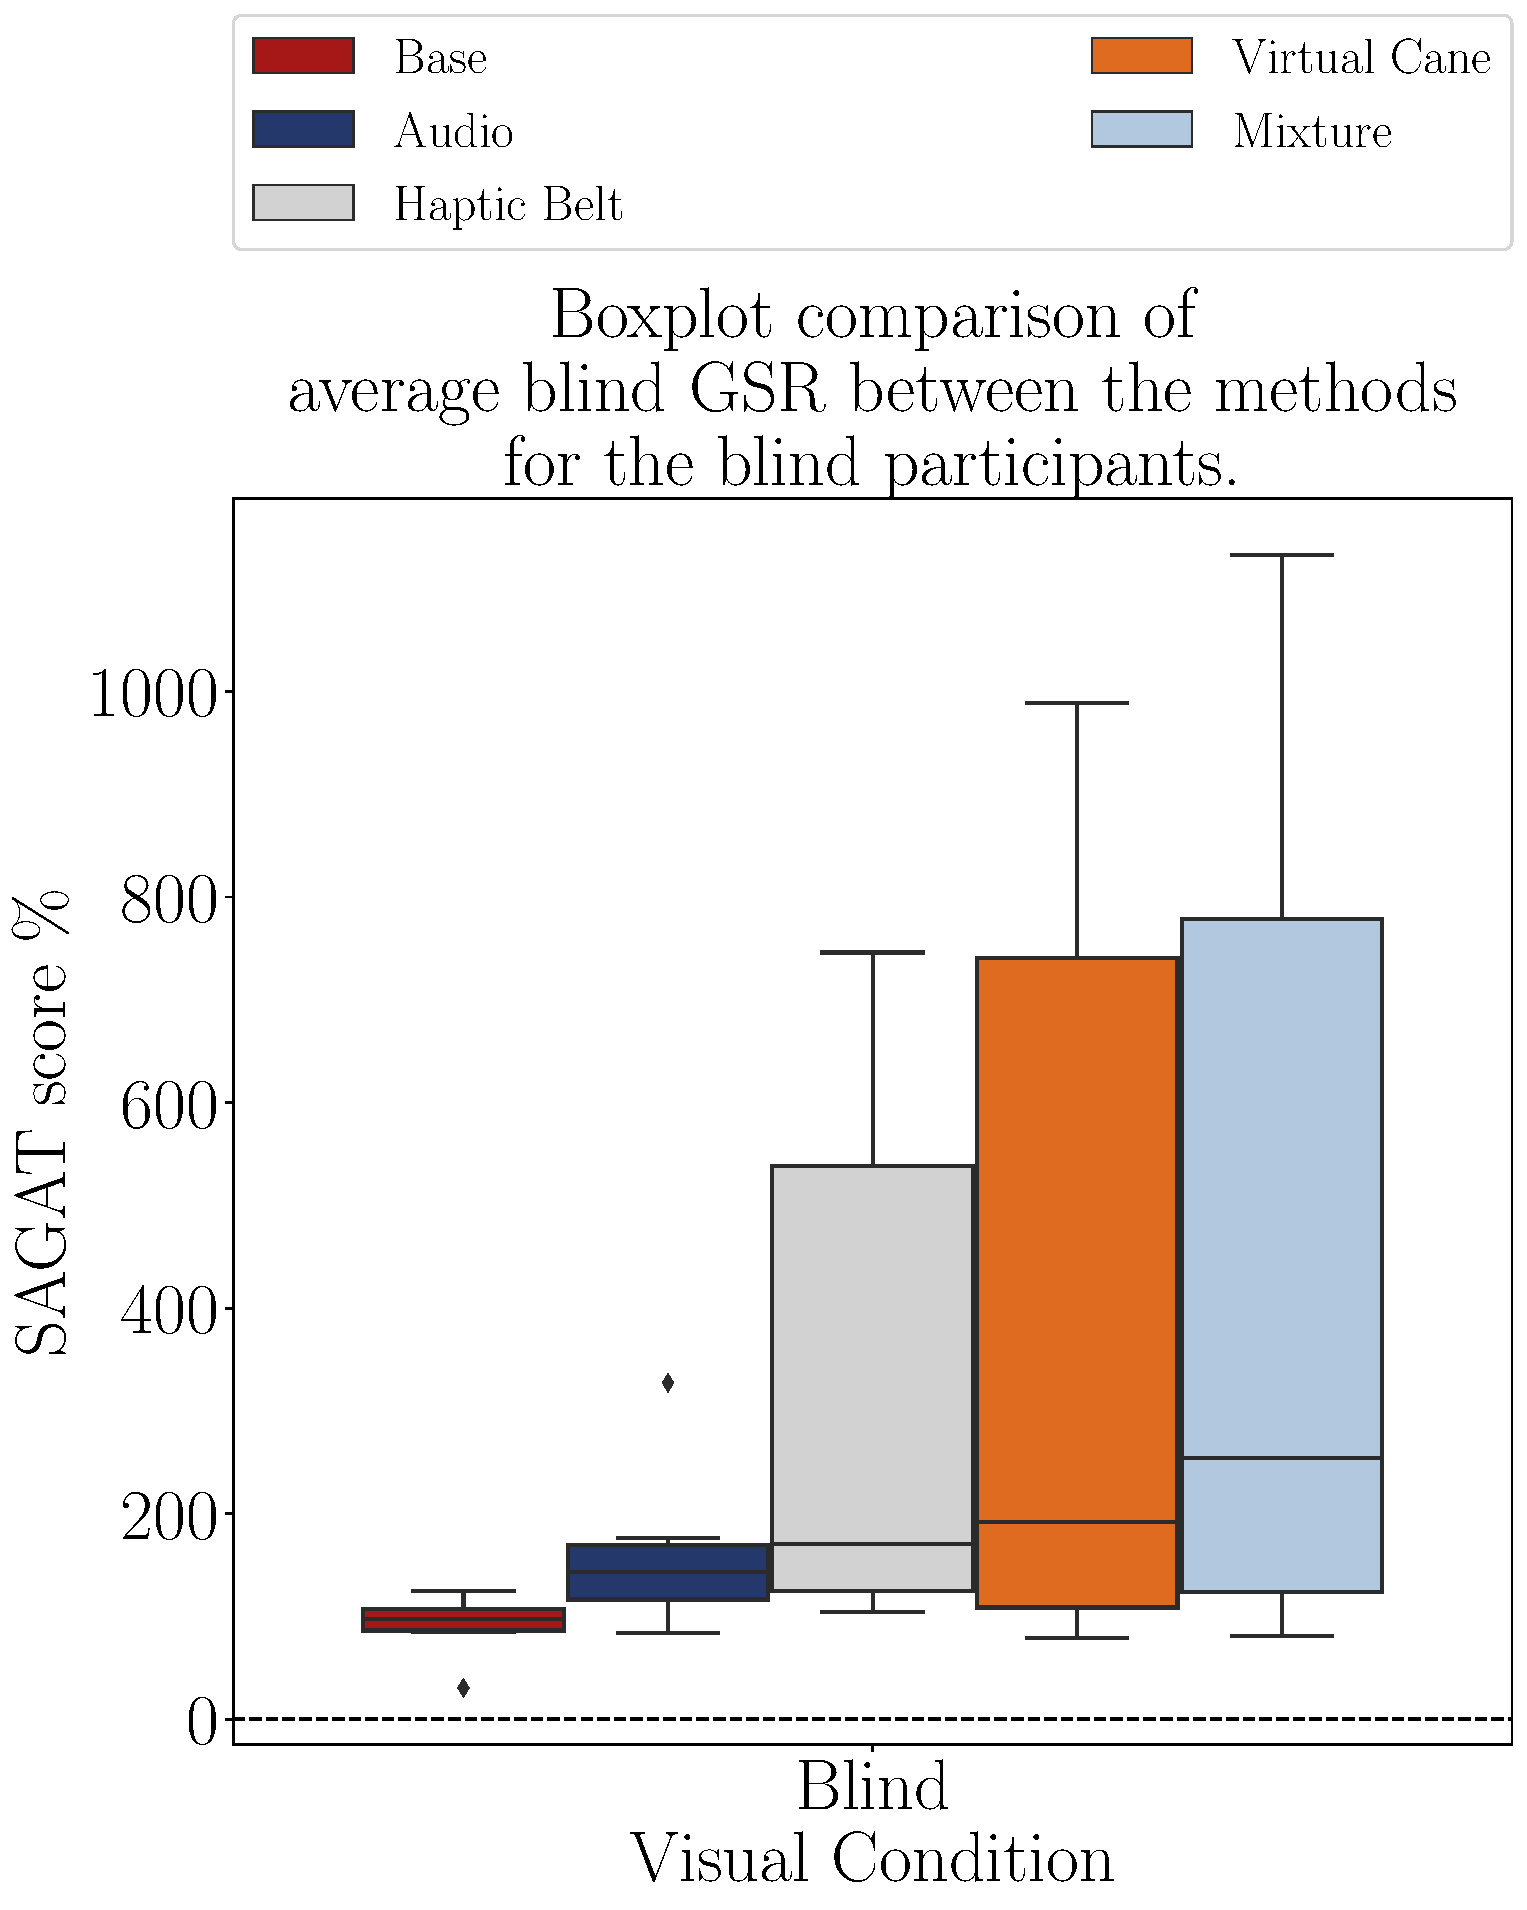
\includegraphics[width = 0.75\linewidth]{3 - Resultados/Figuras/boxplot_gsr_avg_blind_scene.pdf}
    \caption{Boxplot of the GSR of the blind participants grouped by the methods.}
    \label{fig:boxplot_gsr_avg_blind_scene}
\end{figure}
\begin{figure}[!htb]
    \centering
    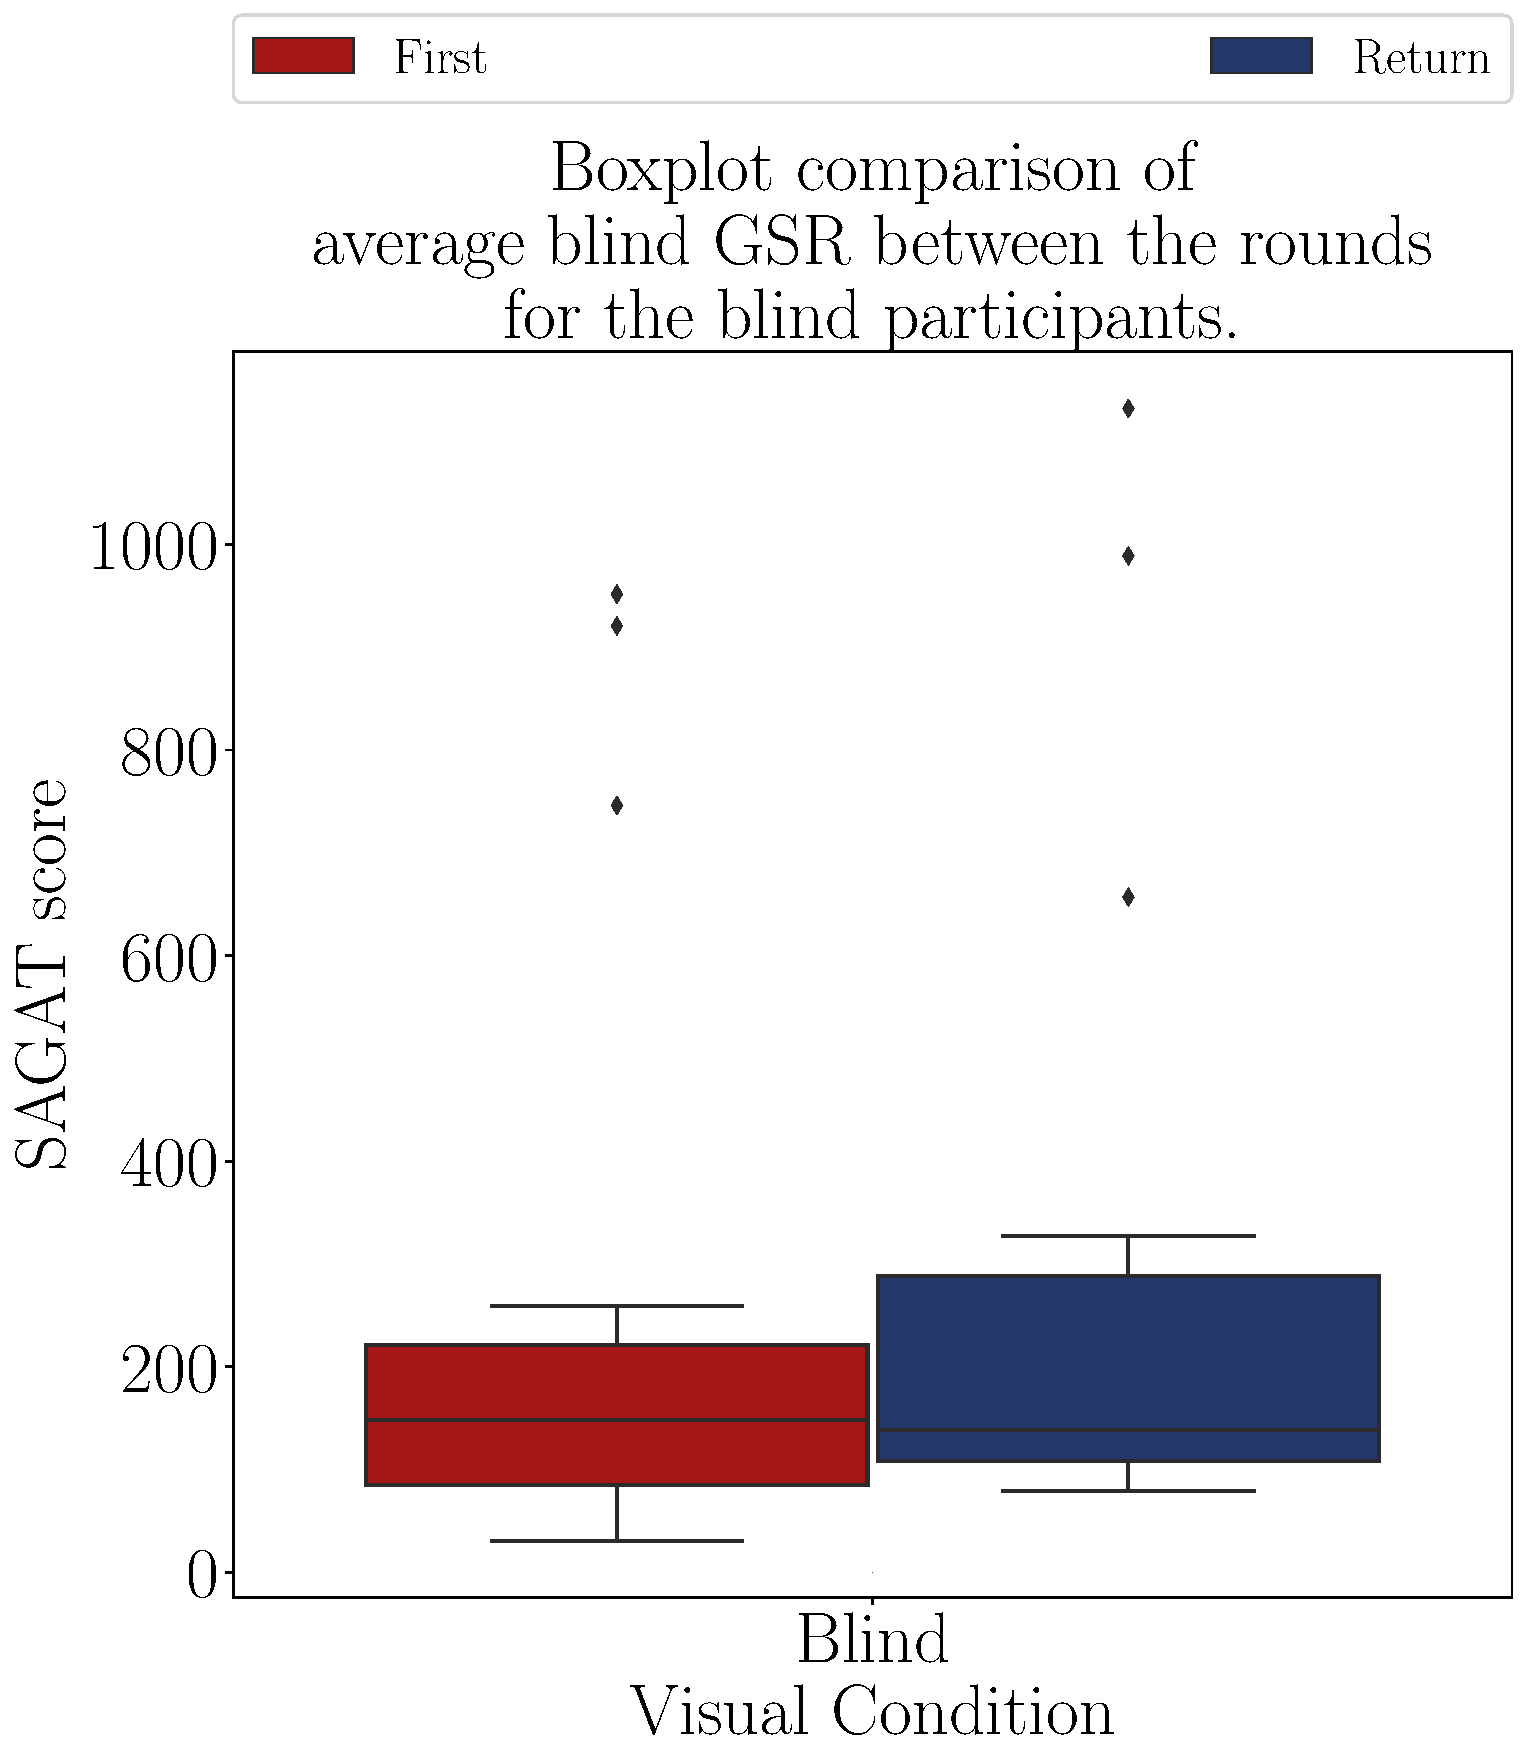
\includegraphics[width = 0.75\linewidth]{3 - Resultados/Figuras/boxplot_gsr_avg_blind_rounds.pdf}
    \caption{Boxplot of the GSR of the blind participants grouped by the rounds.}
    \label{fig:boxplot_gsr_avg_blind_rounds}
\end{figure}

Table \ref{tab:blocanova_gsr_two_way_blind} shows the ANOVA test p-value for the GSR percentual variance. Although the p-value for the method is not below the threshold of 0.05, it is close to it, indicating that probably the GSR is affected by it. 


\begin{table}[!htb]
\centering
\caption{Anova p-value for the mental demand average on each method for blinded users.}
\label{tab:blocanova_gsr_two_way_blind}
\begin{tabular}{lrrrrl}
\toprule
          Source & P-Value \\
\midrule
    \    Methods &   0.051 \\
     \    Rounds &   0.722 \\
\    Interaction &   0.996 \\
\bottomrule
\end{tabular}
\end{table}






%\subsubsection*{Final Remarks}
%
%To summarize the conclusion obtained from the analysis of the data from blind participants, %the audio method showed a lower score both for NASA-TLX mental demand and NASA-TLX global %score. In contrast, the methods that include vibration achieved higher scores. This probably %happened because the participants are already used to using sound to guide themselves, %especially environmental sounds. The environment sounds used in the scenes were always the %same (telephone ringing, laptop keyboard sounds, exterior noise, door opening and closing). %The participants likely felt more relaxed when they only had to focus on the sounds around %him/her. This is reinforced by the fact that, during the experiment with the audio method, %half of the participants did not ask for any information, or the audio command option was %used only a few times.
%
%The fact that the haptic devices caused a higher workload is probably due to the fact that %the users had to learn and get used to them. Besides, for being just conceptual, their %precision was not as good as they were expecting. That explains why their results were not %as good as the base or audio methods. The NASA-TLX results are correctly related to the %satisfaction questionnaires, which scored them as the unsatisfied devices.
%
%As expected, most of the variables from subjective questionnaires (NASA-TLX and SAGAT) show %some influence of the rounds. On the other hand, the results from the physiological sensors %did not show a clear tendency. 
%
%The statistical analysis based on ANOVA tests confirmed some of the observations from the %bar and box plots. However, in many cases, the residual distributions were not homogenous %and the statistical analysis was affected by the small number of samples. 
%
%All the blind participants showed great enthusiasm before, during and after the experiment. %They also made several recommendations for both the virtual environment and the devices, %such as:
%
%\begin{itemize}
%    \item The speakers of the HMD are not good enough to give them the precise location of %the sound origin
%    \item The HMD is too large and covers half of the participant's face. It gives them a strange sensation, since some of them use the air or the wind feeling on the face to give them hints about the location of walls or other high obstacles;
%    \item The precision of the vibration for both the haptic belt and the virtual cane needs to be improved. It is not enough for them to use the devices. This problem is related to %how the HMD sets the position of the user in the virtual environment. \\    
%    \item The vibration from the haptic belt was not intense enough.
%\end%{itemize}

\subsection{Comparison between BVI users and sighted users}
\label{sec:results_obj_2}

This section investigates the second research question of this work: “do non-BVI users, when deprived of their vision, similarly evaluate assistive devices as BVI users?”. 

To do so, the analysis performed in the previous section is now repeated with the data obtained from sighted participants. However, the data corresponding to the "base" method is omitted, as the daily method used by sighted people is based on their vision.

%\subsection{Subjective data}

Only two of the questionnaires will be analyzed, the NASA-TLX and the Adapted SAGAT, and it is expected that for:

\begin{itemize}
    \item \nameref{subsubsec:results_nasa_tlx_2};
    
        There will be a noticeable difference between the sight sample mental workload and the blind sample mental workload.

    \item \nameref{subsubsec:results_adapted_sagat_2};
    
        Is expected to notice a difference between the “blind” sample and the “sight” sample.

    \item \nameref{subsubsec:results_questionnaires}.

        Meant to assess the user experience with each method.

\end{itemize}

\subsection{NASA-TLX}
\label{subsubsec:results_nasa_tlx_2}

\subsubsection{Analysis of the mental demand scale}\mbox{}\\

Table \ref{tab:md_table_noBase} presents the mental demand score of all participants, while the corresponding barplot is presented in Figure \ref{fig:barplot_md_avg_4_scene_blind_sight}. As said before, the higher the value, the higher is the mental demand of the user. It is interesting to observe that sighted people gave a higher score to audio, as they are not so familiar with using sounds as source of guidance.

\input{Resultados/Nasa/Tabelas/md_table_noBase}

\begin{figure}[!thb]
    \centering
    \begin{minipage}{\textwidth}
        \centering
        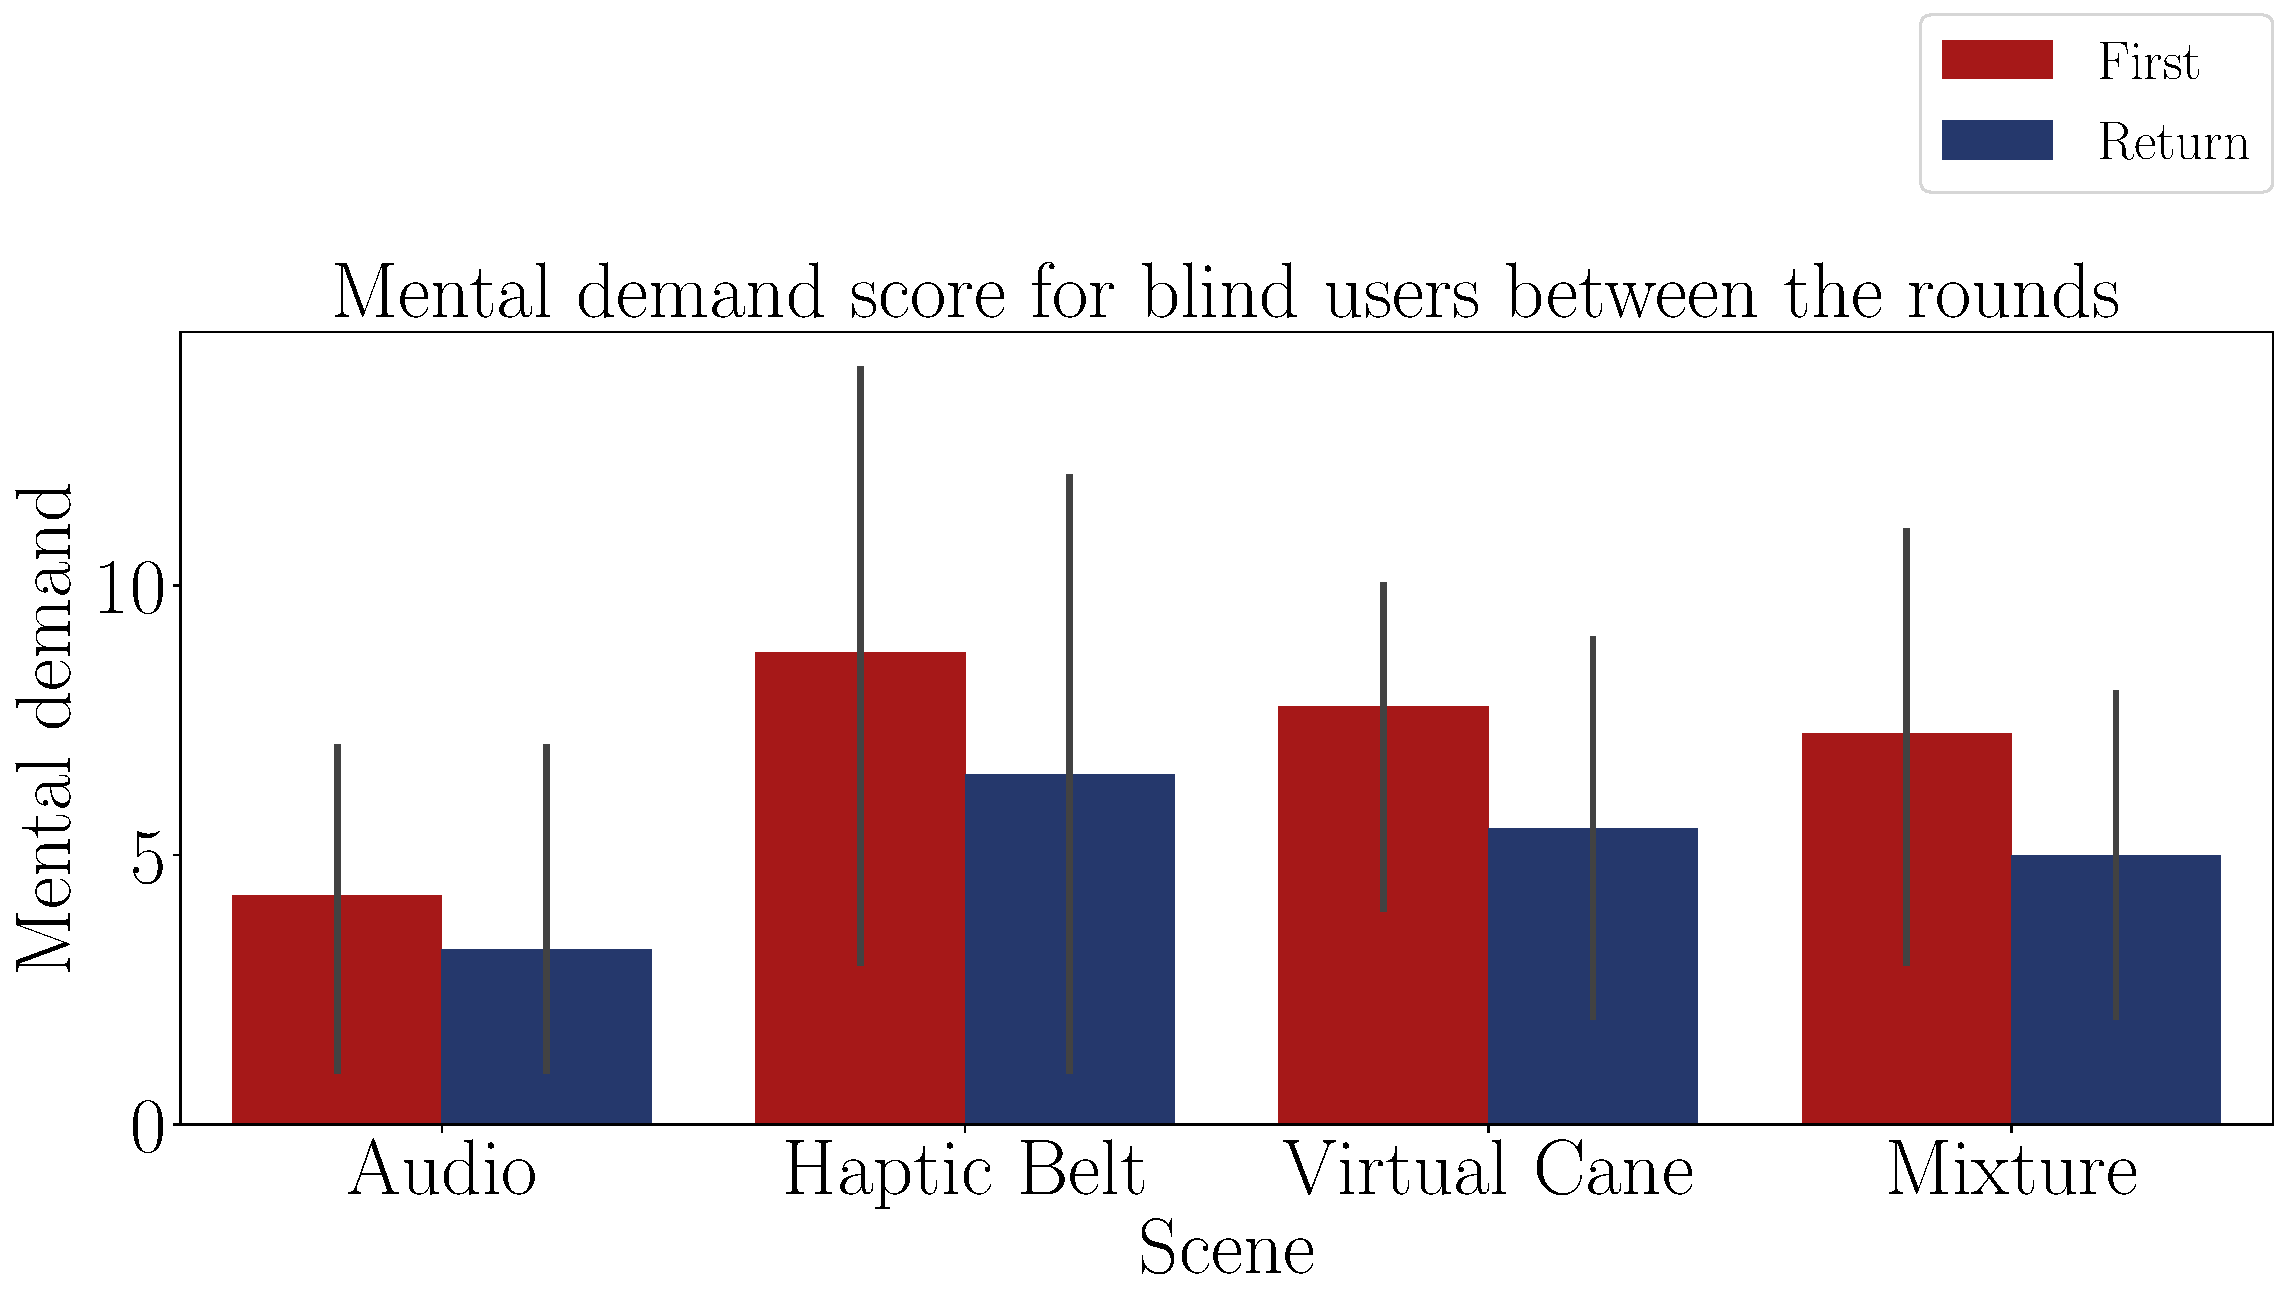
\includegraphics[width = \textwidth]{Resultados/Nasa/Figuras/pdf/barplot_md_avg_4_scene_blind.pdf}
        \subcaption{Blind participants}
        \label{fig:barplot_md_avg_4_scene_blind}
    \end{minipage}
    \begin{minipage}{\textwidth}
        \centering
        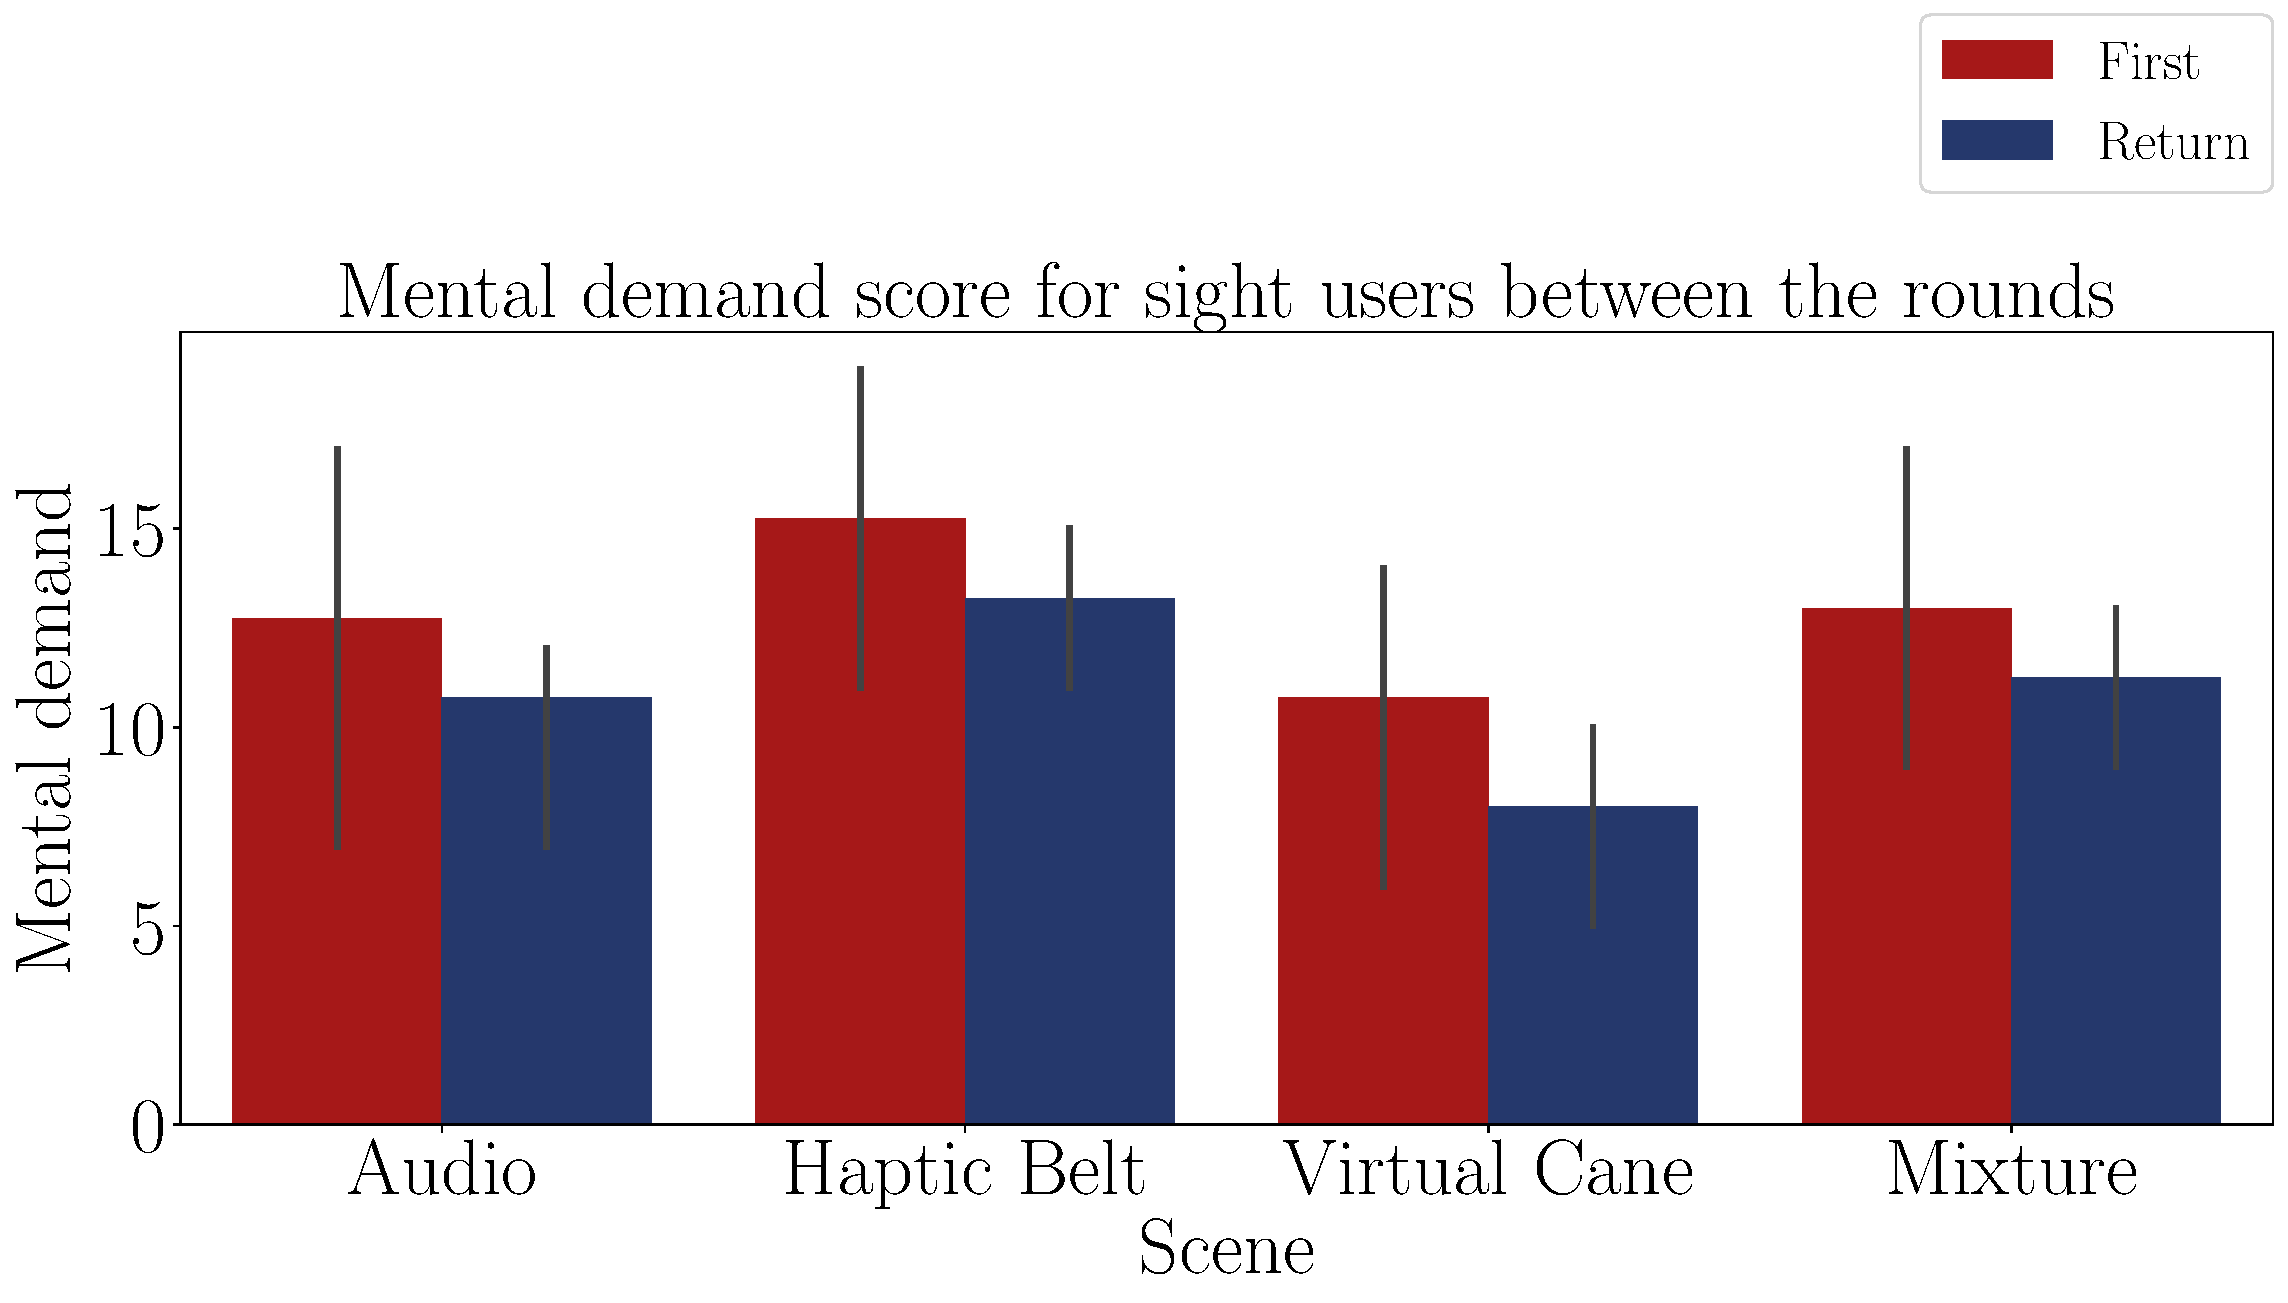
\includegraphics[width = \textwidth]{Resultados/Nasa/Figuras/pdf/barplot_md_avg_4_scene_sight.pdf}
        \subcaption{Sight participants}
        \label{fig:barplot_md_avg_4_scene_sight}
    \end{minipage}
    \caption{Barplot of the average mental demand on each method and each round.}
    \label{fig:barplot_md_avg_4_scene_blind_sight}
\end{figure}

Figures \ref{fig:boxplot_noBase_md_4_scene} and \ref{fig:boxplot_noBase_md_4_rounds} presents the box plot for both groups, organized by the methods and the rounds. The mental demand is systematically higher for sighted people, which is expected. However, while blind participants considered the audio method less demanding, sighted participants prefered to the virtual cane. For both groups, we observe a decrease in the mental demand.

\begin{figure}[!htb]
    \centering
    \begin{minipage}{0.45\textwidth}
        \centering
        \includegraphics[width = \textwidth]{Resultados/Nasa/Figuras/pdf/boxplot_noBase_md_4_scene.pdf}
        \caption{Boxplot of the mental demand of the participants grouped by the methods.}
        \label{fig:boxplot_noBase_md_4_scene}
    \end{minipage}
    \begin{minipage}{0.075\textwidth}
        \hfill
    \end{minipage}
    \begin{minipage}{0.45\textwidth}
        \centering
        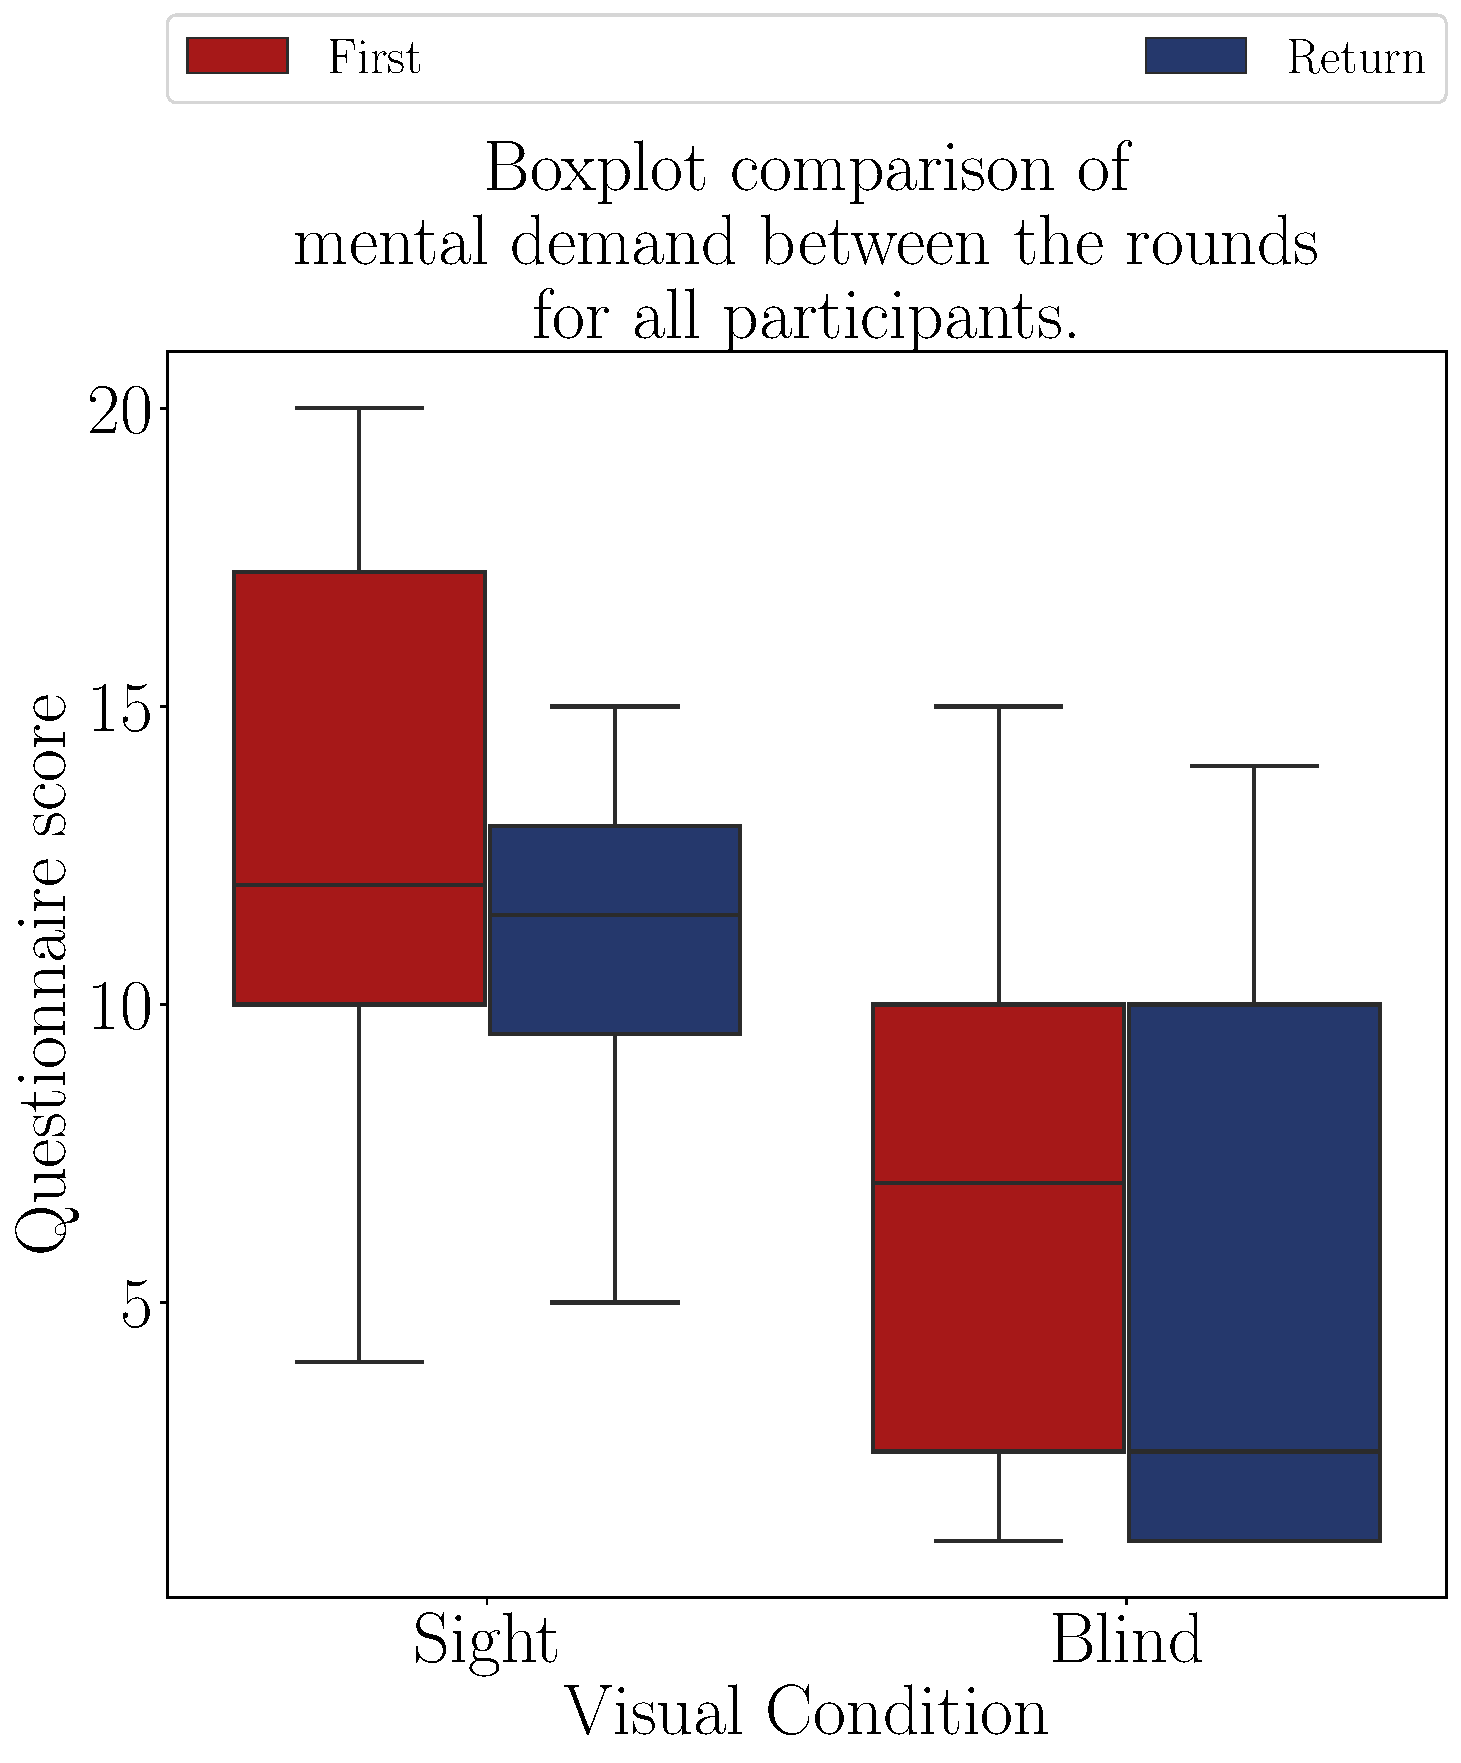
\includegraphics[width = \textwidth]{Resultados/Nasa/Figuras/pdf/boxplot_noBase_md_4_rounds.pdf}
        \caption{Boxplot of the mental demand of the participants grouped by the rounds.}
        \label{fig:boxplot_noBase_md_4_rounds}
    \end{minipage}
\end{figure}

Figures \ref{fig:qqplot_md_avg_two_way_sight} and \ref{fig:residplot_md_avg_two_way_sight} show the QQ plot and residual distribution for the sighted data, confirming that the data is normally distributed and participants have similar variance. Table \ref{tab:blocanova_md_avg_two_way_blind_sight} brings the results of ANOVA. Unlike the blind participants, in the case of sighted ones, the p-value for the methods is below the threshold of 0.05, confirming it as a significant variable for the mental demand. In the case of the rounds, the data from both sighted and blind participants resulted in the exact p-value of 0.075, which is close to the traditional threshold of 0.05 but slightly higher. 

\begin{table}[!htb]
    \caption{Anova p-value for the mental demand average on each method'}
    \label{tab:blocanova_md_avg_two_way_blind_sight}
\begin{minipage}{0.45\textwidth}
    \subcaption{Blind participants}
    \input{Resultados/Nasa/Tabelas/blocanova_md_avg_two_way_blindSemBegin.tex}
\end{minipage}
\begin{minipage}{0.45\textwidth}
    \subcaption{Sight participants}
    \input{Resultados/Nasa/Tabelas/blocanova_md_avg_two_way_sightSemBegin.tex}    
\end{minipage}
\end{table}

\begin{figure}[!htb]
    \centering
    %\vspace{-15.0cm}
    \begin{minipage}{0.45\textwidth}
        \centering
        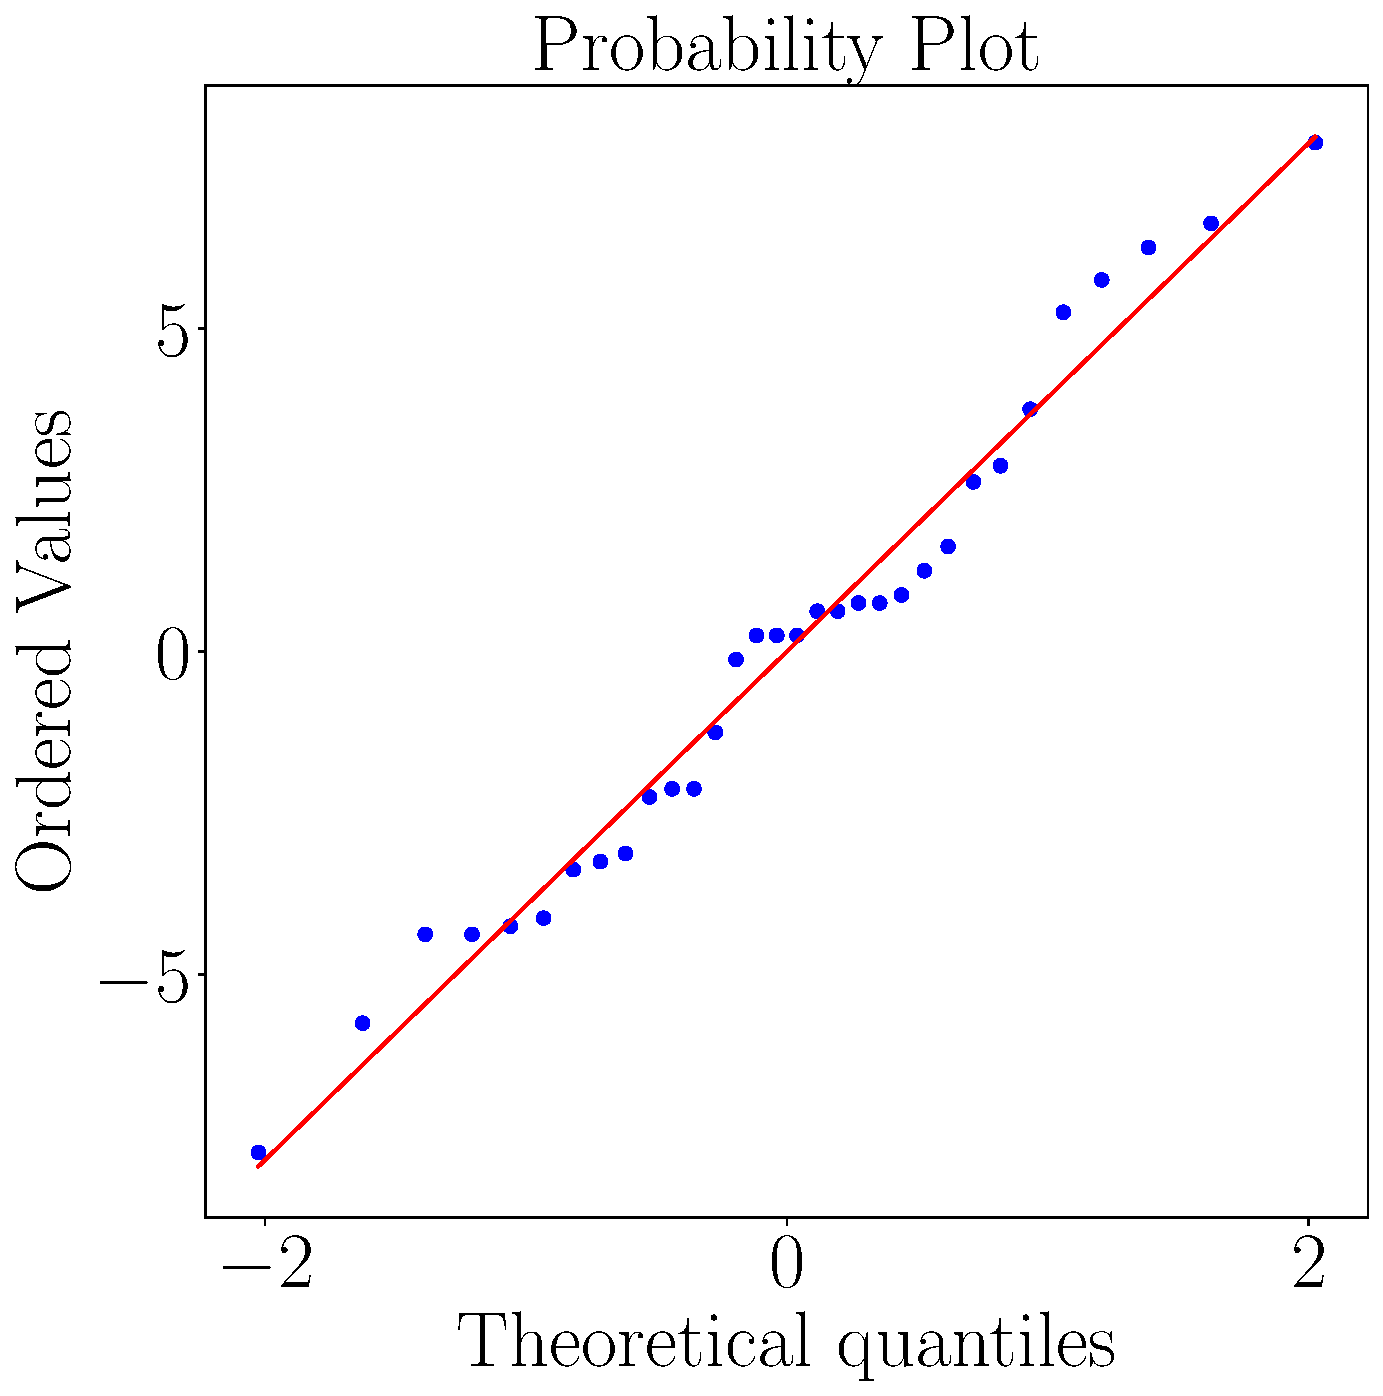
\includegraphics[width = \textwidth]{Resultados/Nasa/Figuras/pdf/qqplot_md_avg_two_way_sight.pdf}
        \caption{QQ plot of the mental demand of the sight participants on each method.}
        \label{fig:qqplot_md_avg_two_way_sight}
    \end{minipage}
    \begin{minipage}{0.075\textwidth}
        \hfill
    \end{minipage}
    \begin{minipage}{0.45\textwidth}
        \centering
        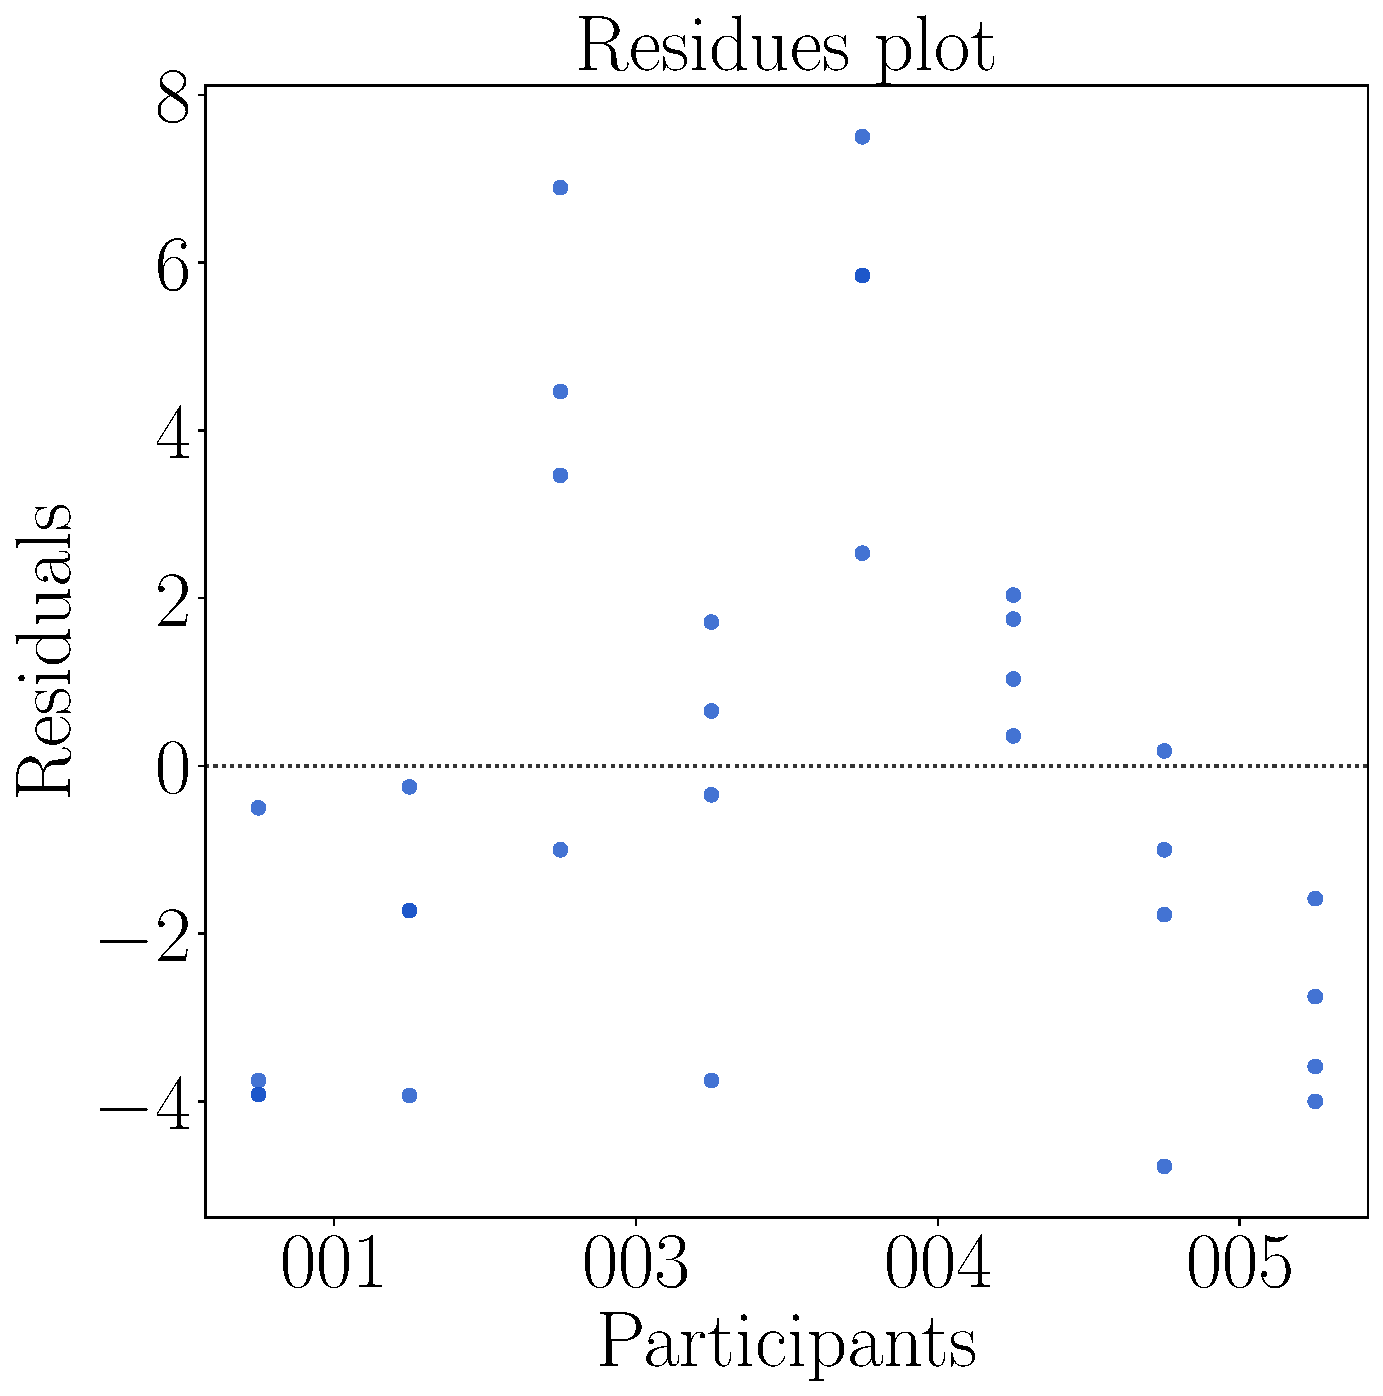
\includegraphics[width = \textwidth]{Resultados/Nasa/Figuras/pdf/residplot_md_avg_two_way_sight.pdf}
        \caption{Residual plot of the mental demand score the sighted participants on each method.}
        \label{fig:residplot_md_avg_two_way_sight}
    \end{minipage}
\end{figure}

\FloatBarrier

%%%%%%%%%%%%%%%%%%%%%%%%%%%%%%%%%%%%%%%%%%%%%%%%%%%%%%%%%%%%%%%%%%%%%%%%%%%%
%%%%%%%%%%%%%%%%%%%%%%%%%%%%%%%%%%%%%%%%%%%%%%%%%%%%%%%%%%%%%%%%%%%%%%%%%%%%
%%%%%%%%%%%%%%%%%%%%%%%%%%%%%%%%%%%%%%%%%%%%%%%%%%%%%%%%%%%%%%%%%%%%%%%%%%%%
%%%%%%%%%%%%%%%%%%%%%%%%%%%%%%%%%%%%%%%%%%%%%%%%%%%%%%%%%%%%%%%%%%%%%%%%%%%%


\subsubsection{Analysis of the NASA-TLX score}\mbox{}\\

Table \ref{tab:nasa_table_noBase} brings the NASA-TLX global score of all participants, while the corresponding barplot is presented in Figure \ref{fig:barplot_nasa_avg_4_scene}. As before, the higher the value, the higher is the Mental Workload of the user.

\input{Resultados/Nasa/Tabelas/nasa_table_noBase}

From Figure \ref{fig:barplot_nasa_avg_4_scene}, it is possible to see that, similar to blind participants, sighted participants consider that the workload of the return round was lower than that of the first round. However, similar to what happened for the mental demand, sighted participants considered virtual cane as the methods with the lowest workload, while, for  blind participants, it was the audio.

\begin{figure}[!htb]
    \centering
    \begin{minipage}{\textwidth}
        \centering
        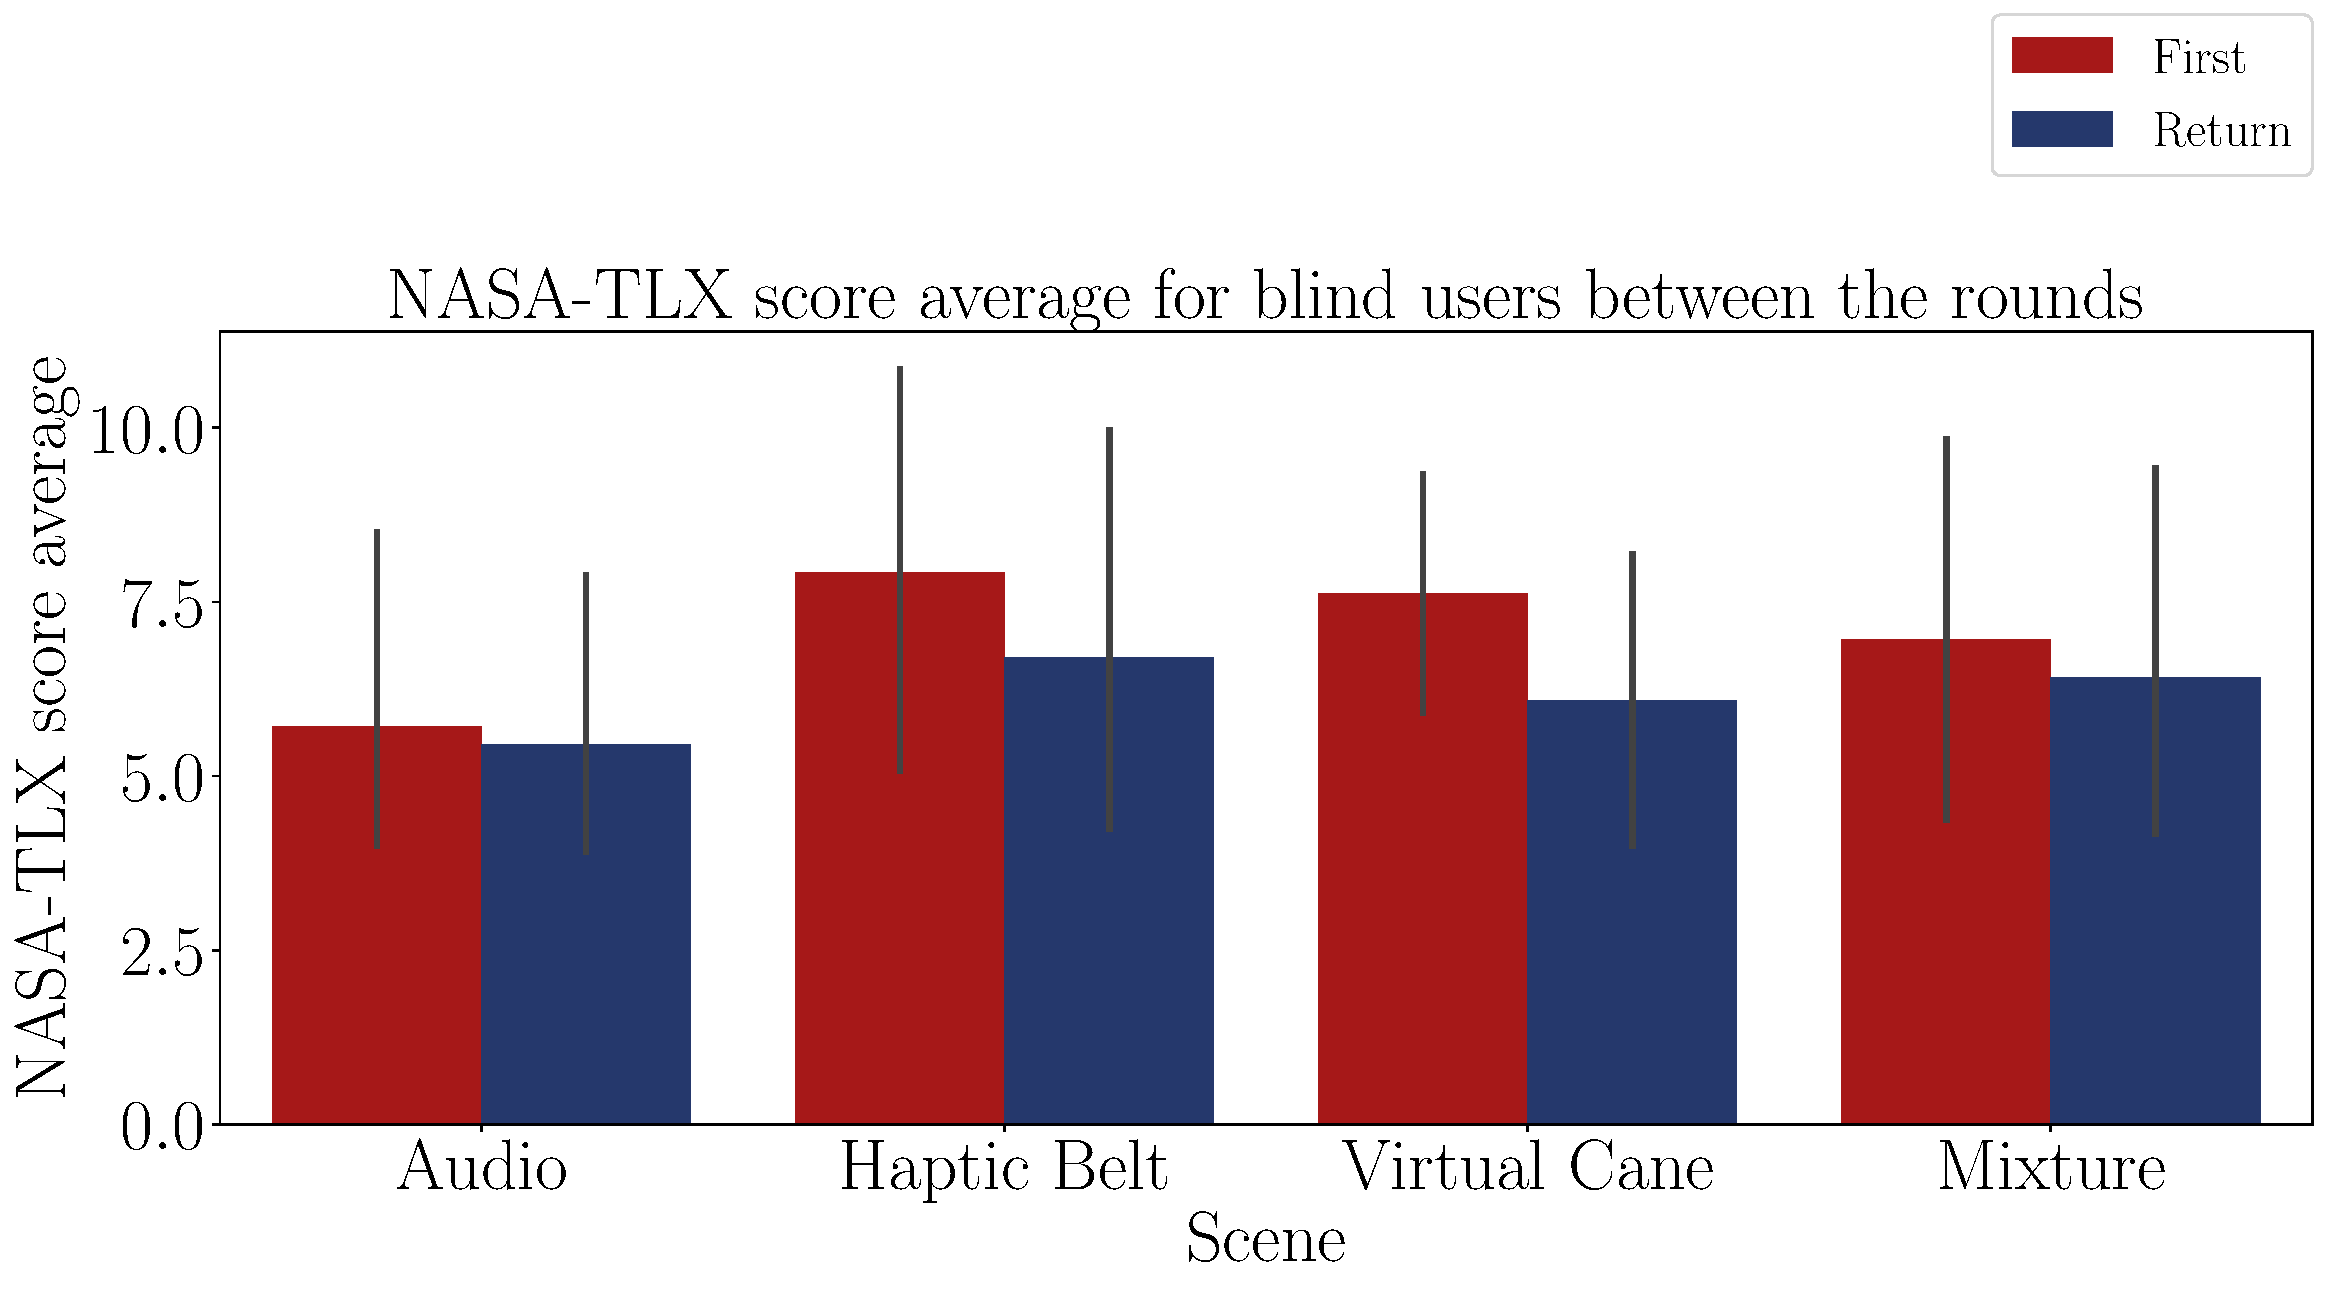
\includegraphics[width = \textwidth]{Resultados/Nasa/Figuras/pdf/barplot_nasa_avg_4_scene_blind.pdf}
        \subcaption{Blind participants.}
        \label{fig:barplot_nasa_avg_4_scene_blind}
    \end{minipage}
    \begin{minipage}{\textwidth}
        \centering
        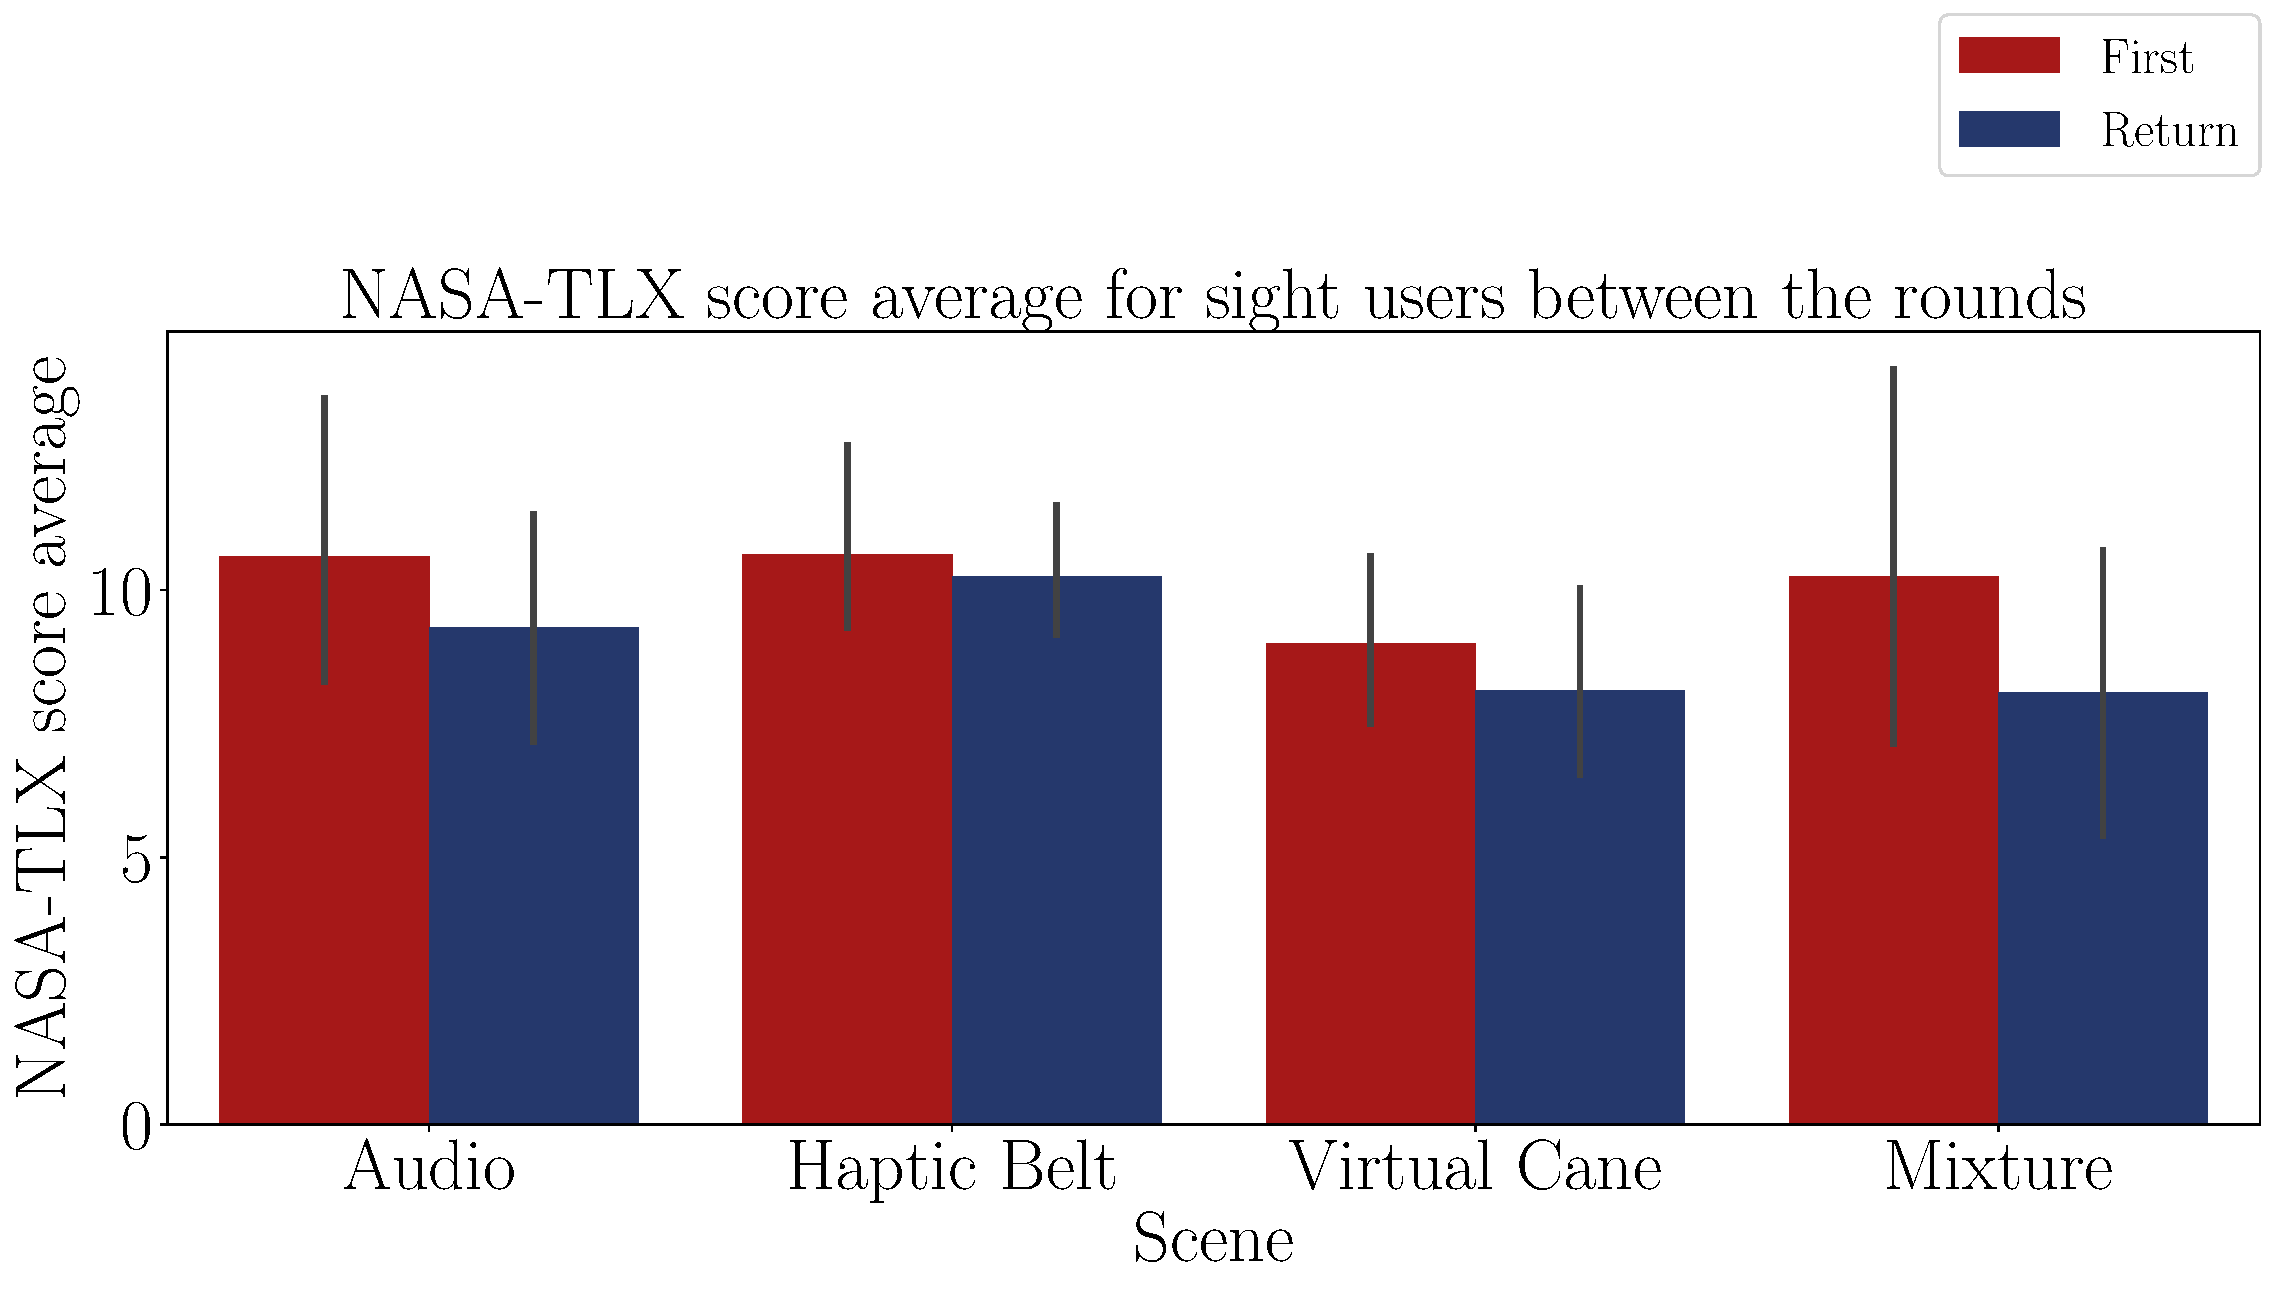
\includegraphics[width = \textwidth]{Resultados/Nasa/Figuras/pdf/barplot_nasa_avg_4_scene_sight.pdf}
        \subcaption{Sight participants.}
        \label{fig:barplot_nasa_avg_4_scene_sight}
    \end{minipage}
    \caption{Barplot of the NASA-TLX score on each method and each round.}
    \label{fig:barplot_nasa_avg_4_scene}
\end{figure}

Figures \ref{fig:boxplot_noBase_nasa_4_scene} and \ref{fig:boxplot_noBase_nasa_4_rounds} present the boxplots of the NASA-TLX global score. Again, it is possible to see that sighted people usually give higher workload scores than blind ones. The influence of the round is approximately the same. However, the order of preference of the methods is different.

\begin{figure}[!htb]
    \centering
    \begin{minipage}{0.45\textwidth}
        \centering
        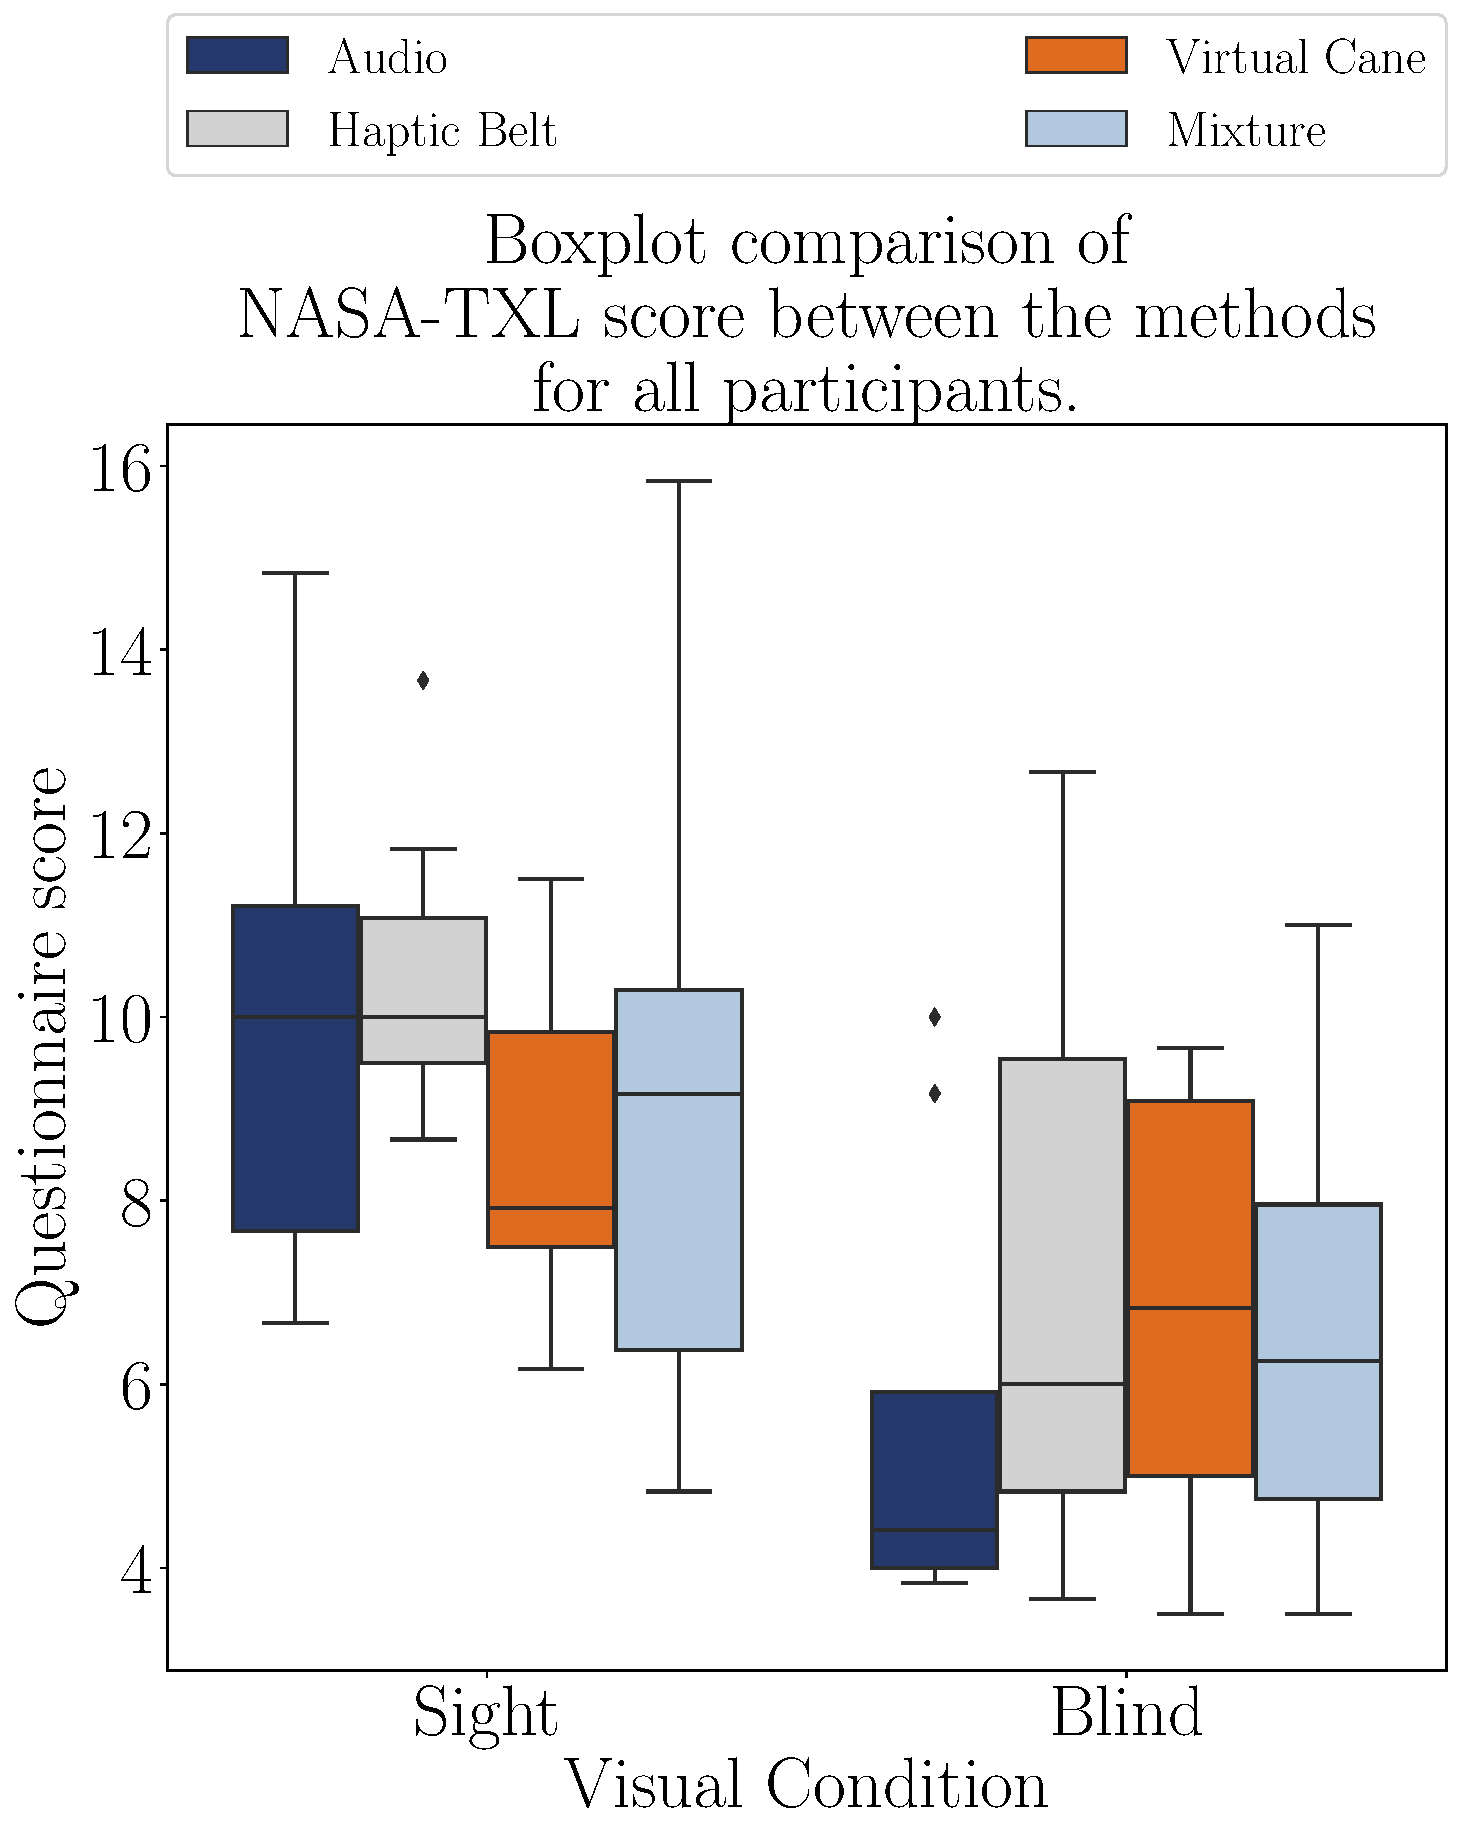
\includegraphics[width = \textwidth]{Resultados/Nasa/Figuras/pdf/boxplot_noBase_nasa_4_scene.pdf}
        \caption{Boxplot of the NASA-TLX score of the participants grouped by the methods.}
        \label{fig:boxplot_noBase_nasa_4_scene}
    \end{minipage}
    \begin{minipage}{0.075\textwidth}
        \hfill
    \end{minipage}
    \begin{minipage}{0.45\textwidth}
        \centering
        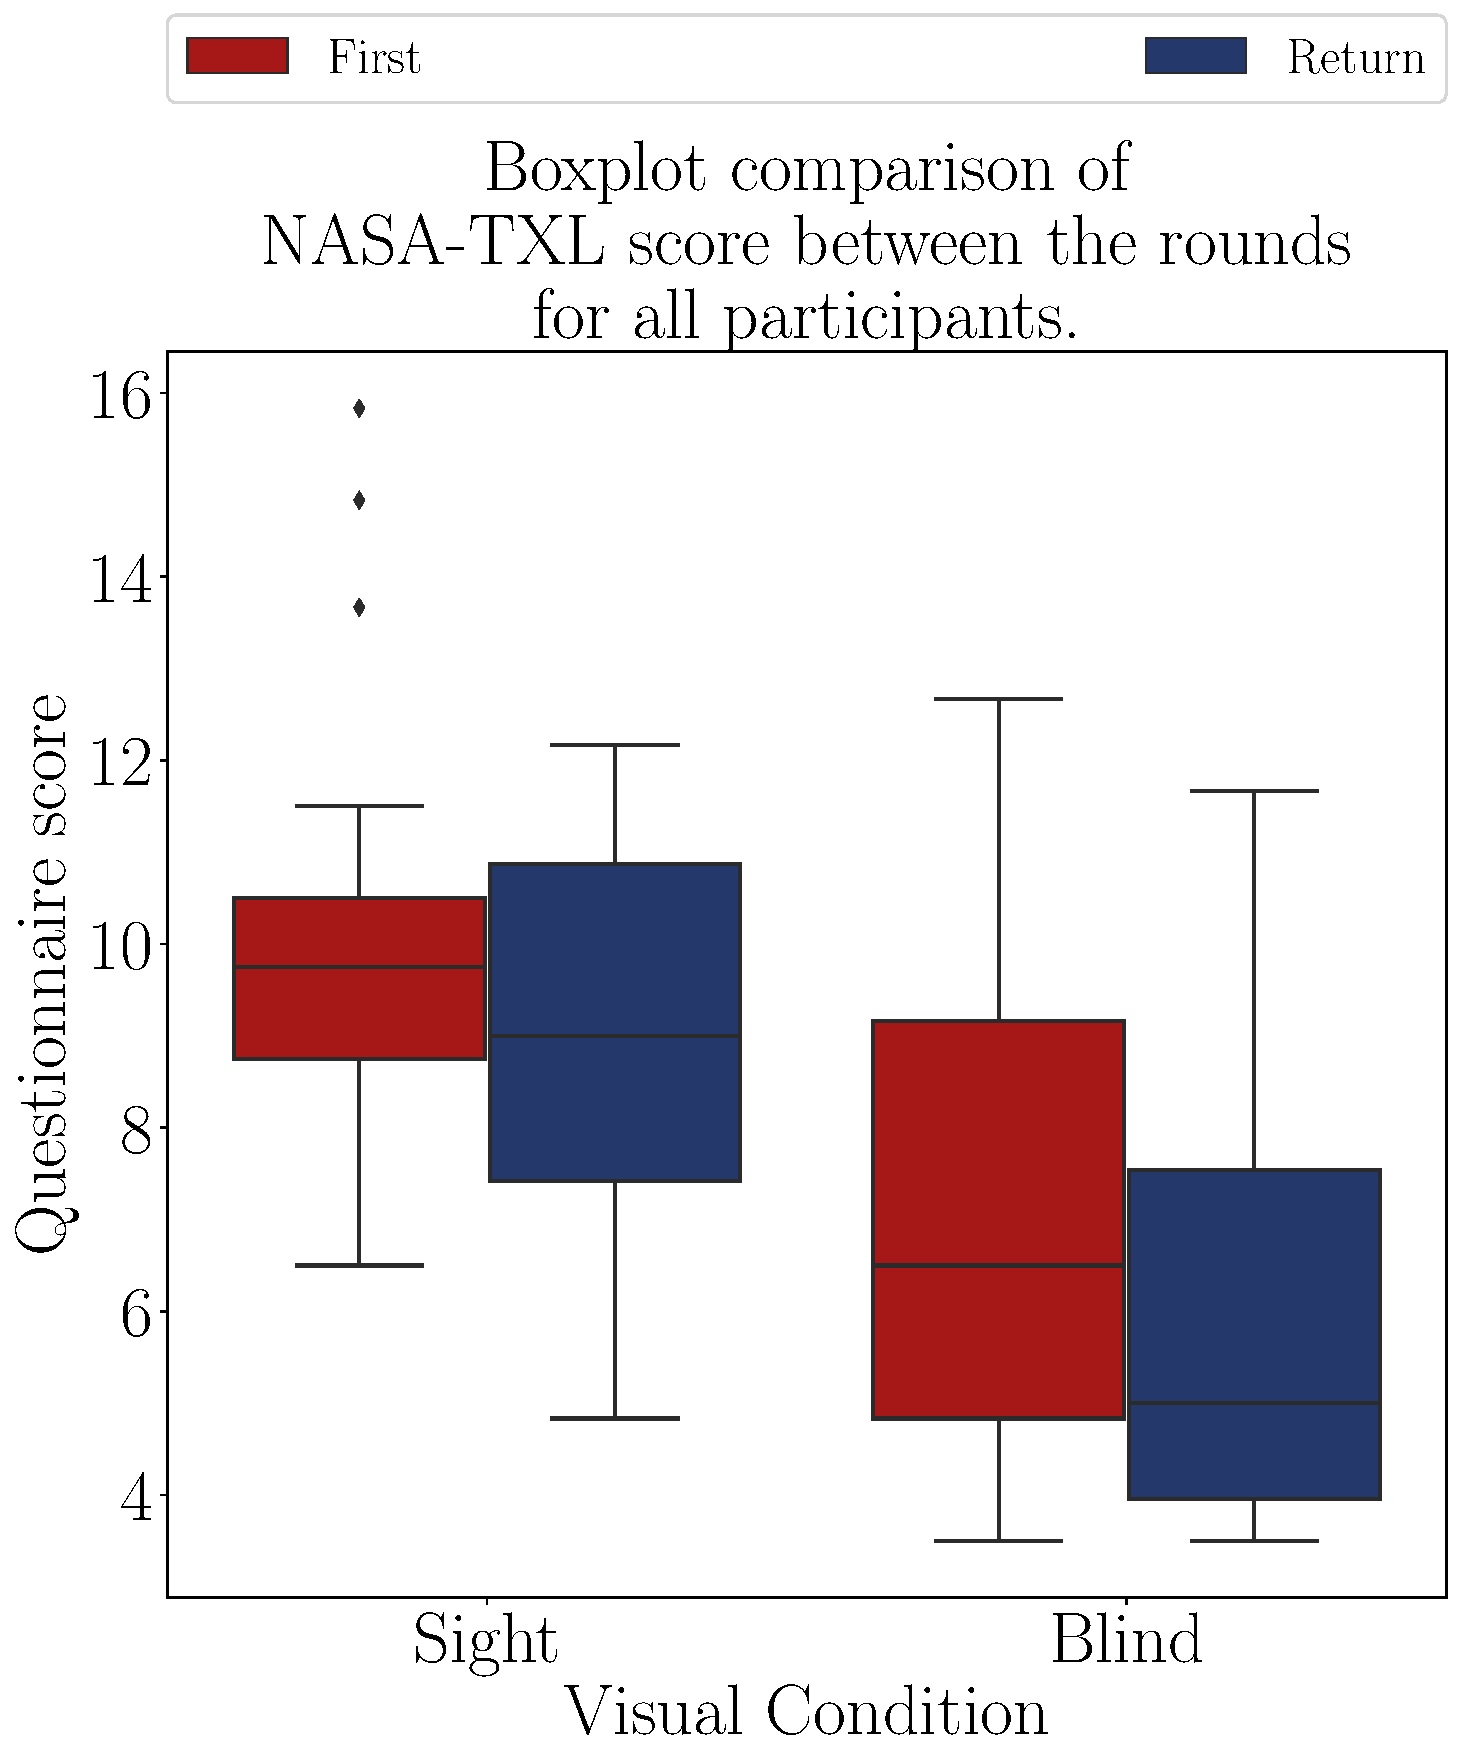
\includegraphics[width = \textwidth]{Resultados/Nasa/Figuras/pdf/boxplot_noBase_nasa_4_rounds.pdf}
        \caption{Boxplot of the NASA-TLX score of the participants grouped by the rounds.}
        \label{fig:boxplot_noBase_nasa_4_rounds}
    \end{minipage}
\end{figure}

Figures \ref{fig:qqplot_nasa_avg_two_way_sight} and \ref{fig:residplot_nasa_avg_two_way_sight} bring the QQ plot and residual distribution of the data from sighted participants, showing that ANOVA can be used. The p-values for both groups are presented in Table \ref{tab:blocanova_nasa_avg_two_way_blind_sight}. It confirms the influence of the round for both sighted and blind people. In the case of the methods, the p-value of blind is lower than the threshold of 0.5, while that of sighted is slightly higher.

\begin{table}[!thb]
    \caption{Anova p-value for the NASA-TLX score on each method}
    \label{tab:blocanova_nasa_avg_two_way_blind_sight}
    \begin{minipage}{0.45\textwidth}
        \subcaption{Blind participants}
        \input{Resultados/Nasa/Tabelas/blocanova_nasa_avg_two_way_blindSemBegin.tex}
    \end{minipage}
    \begin{minipage}{0.45\textwidth}
        \subcaption{Sight participants}
        \input{Resultados/Nasa/Tabelas/blocanova_nasa_avg_two_way_sightSemBegin.tex}    
    \end{minipage}
\end{table}


\begin{figure}[!htb]
    \centering
    %\vspace{-15.0cm}
    \begin{minipage}{0.45\textwidth}
        \centering
        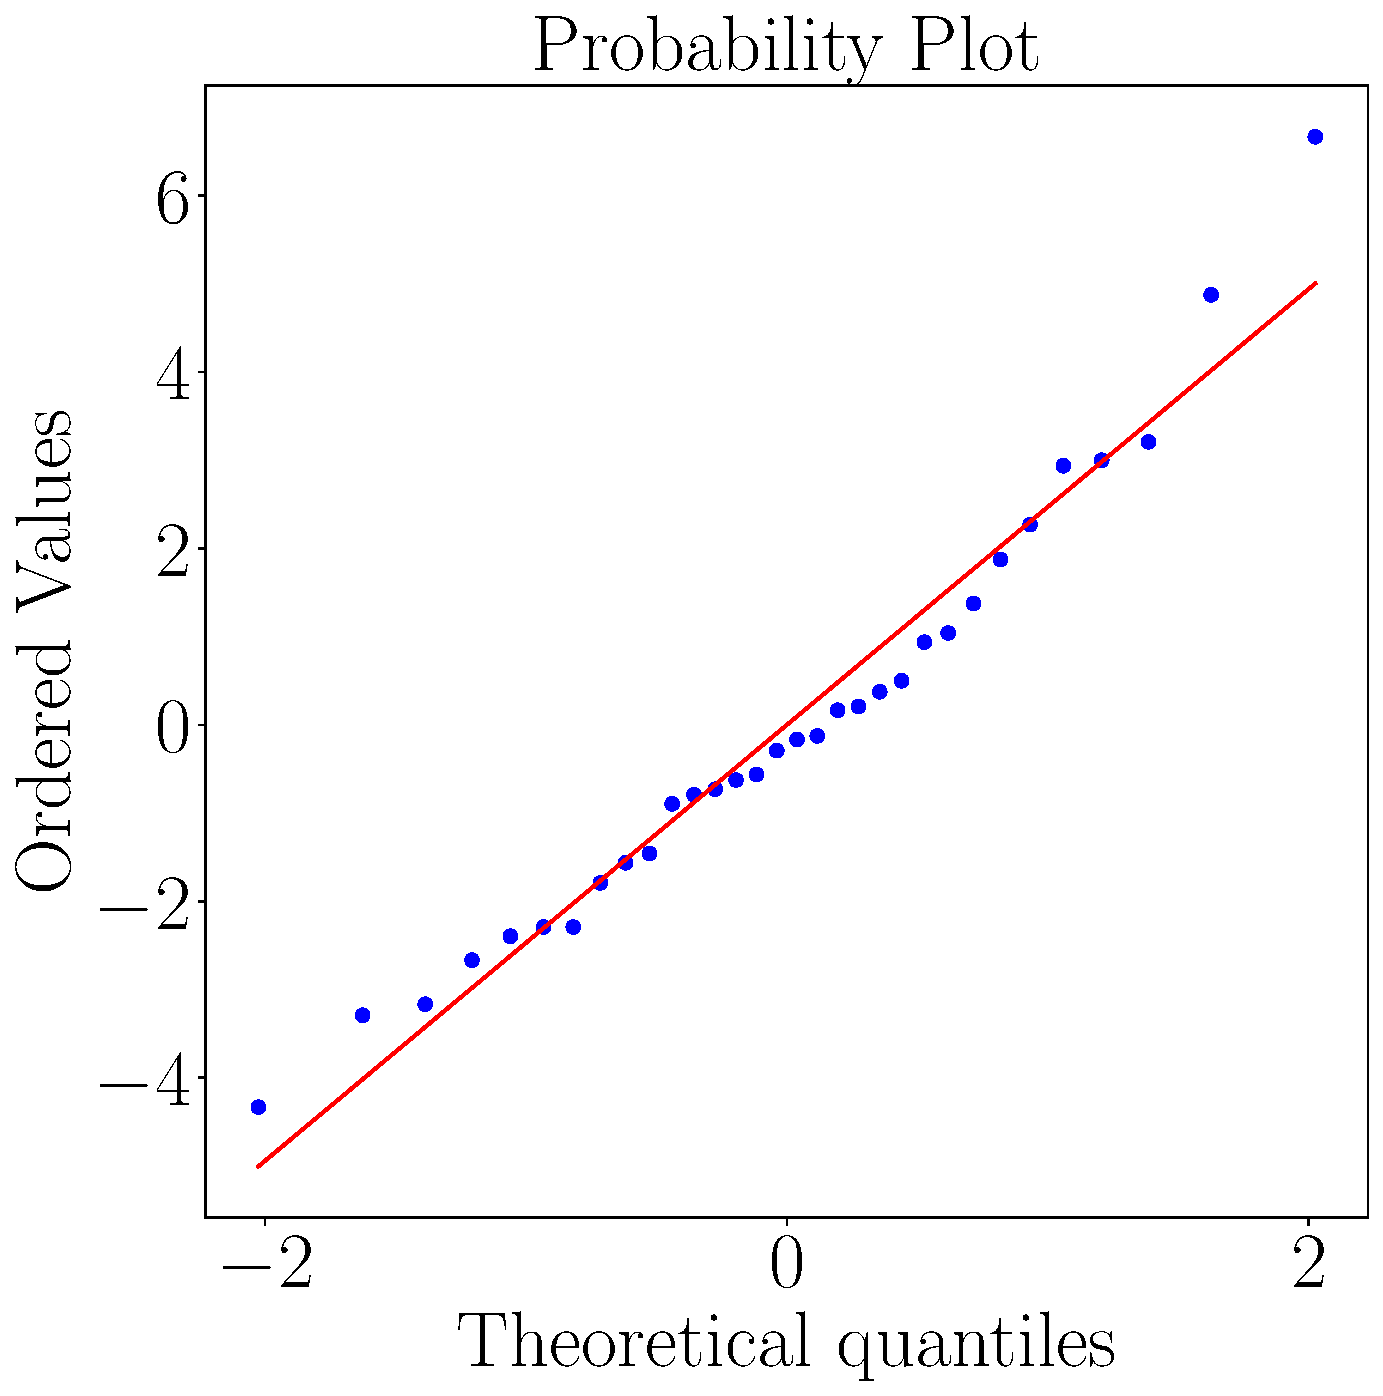
\includegraphics[width = \textwidth]{Resultados/Nasa/Figuras/pdf/qqplot_nasa_avg_two_way_sight.pdf}
        \caption{QQ plot of the NASA-TLX score of the sight participants on each method.}
        \label{fig:qqplot_nasa_avg_two_way_sight}
    \end{minipage}
    \begin{minipage}{0.075\textwidth}
        \hfill
    \end{minipage}
    \begin{minipage}{0.45\textwidth}
        \centering
        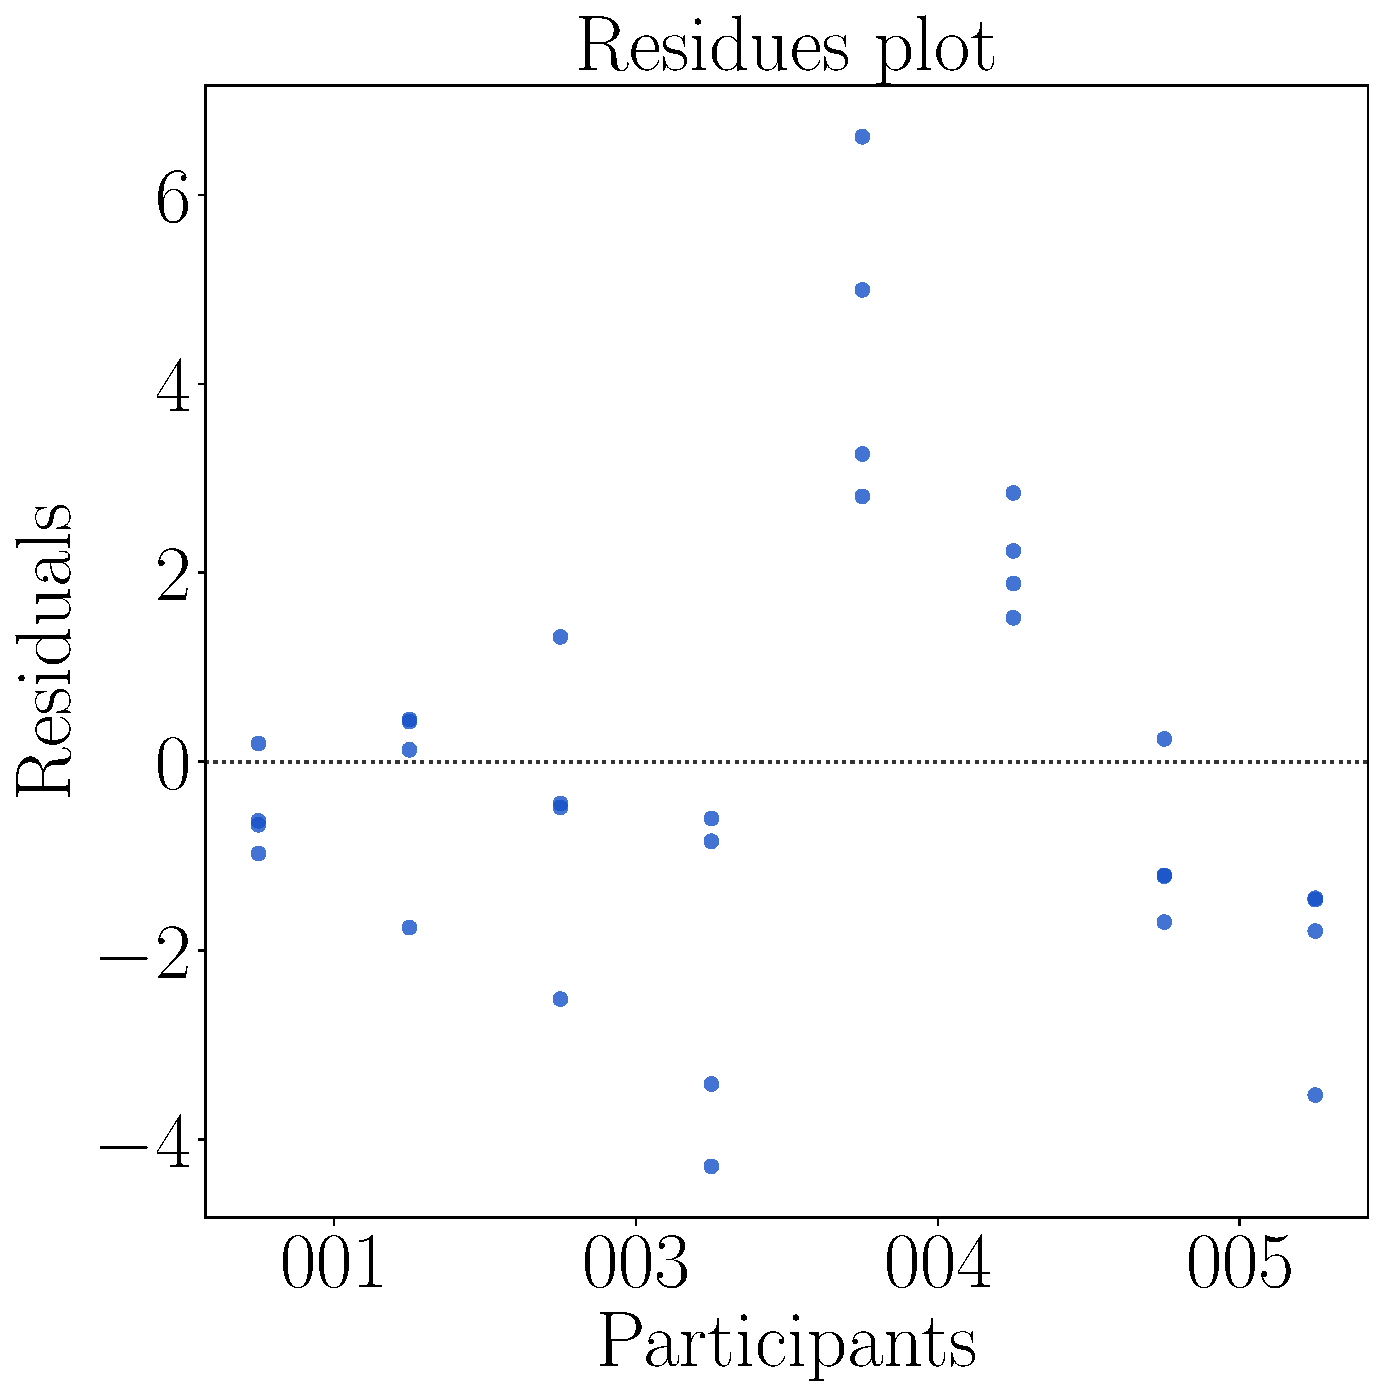
\includegraphics[width = \textwidth]{Resultados/Nasa/Figuras/pdf/residplot_nasa_avg_two_way_sight.pdf}
        \caption{Residual plot of the NASA-TLX score the sight participants on each method.}
        \label{fig:residplot_nasa_avg_two_way_sight}
    \end{minipage}
\end{figure}

\FloatBarrier

\subsubsection{Adapted SAGAT}
\label{subsubsec:results_adapted_sagat_2}

%Table \ref{tab:sagat_table_noBase} presents the SAGAT score of all participants. As said before, the higher the value, the higher is the Situation Awareness of the user. The corresponding barplot is presented in Figure \ref{fig:barplot_sagat_avg_4_scene_blind_sight}.

%\input{Resultados/sagat/Tabelas/sagat_table_noBase}

%Figure \ref{fig:barplot_sagat_avg_4_scene_blind_sight}. shows that the SAGAT score for sighted participants is, on average lower than that of blind participants, which is expected as they are not used to navigating without vision. Also, the increase in situation awareness from the first to the return round is lower. In the case of the mixture method, the SAGAT score did not improve at all. For both groups, the virtual cane was the method with the lowest score in the first round.
%
%\begin{figure}[!htb]
%    \centering
%    \begin{minipage}{\linewidth}
%        \centering
%        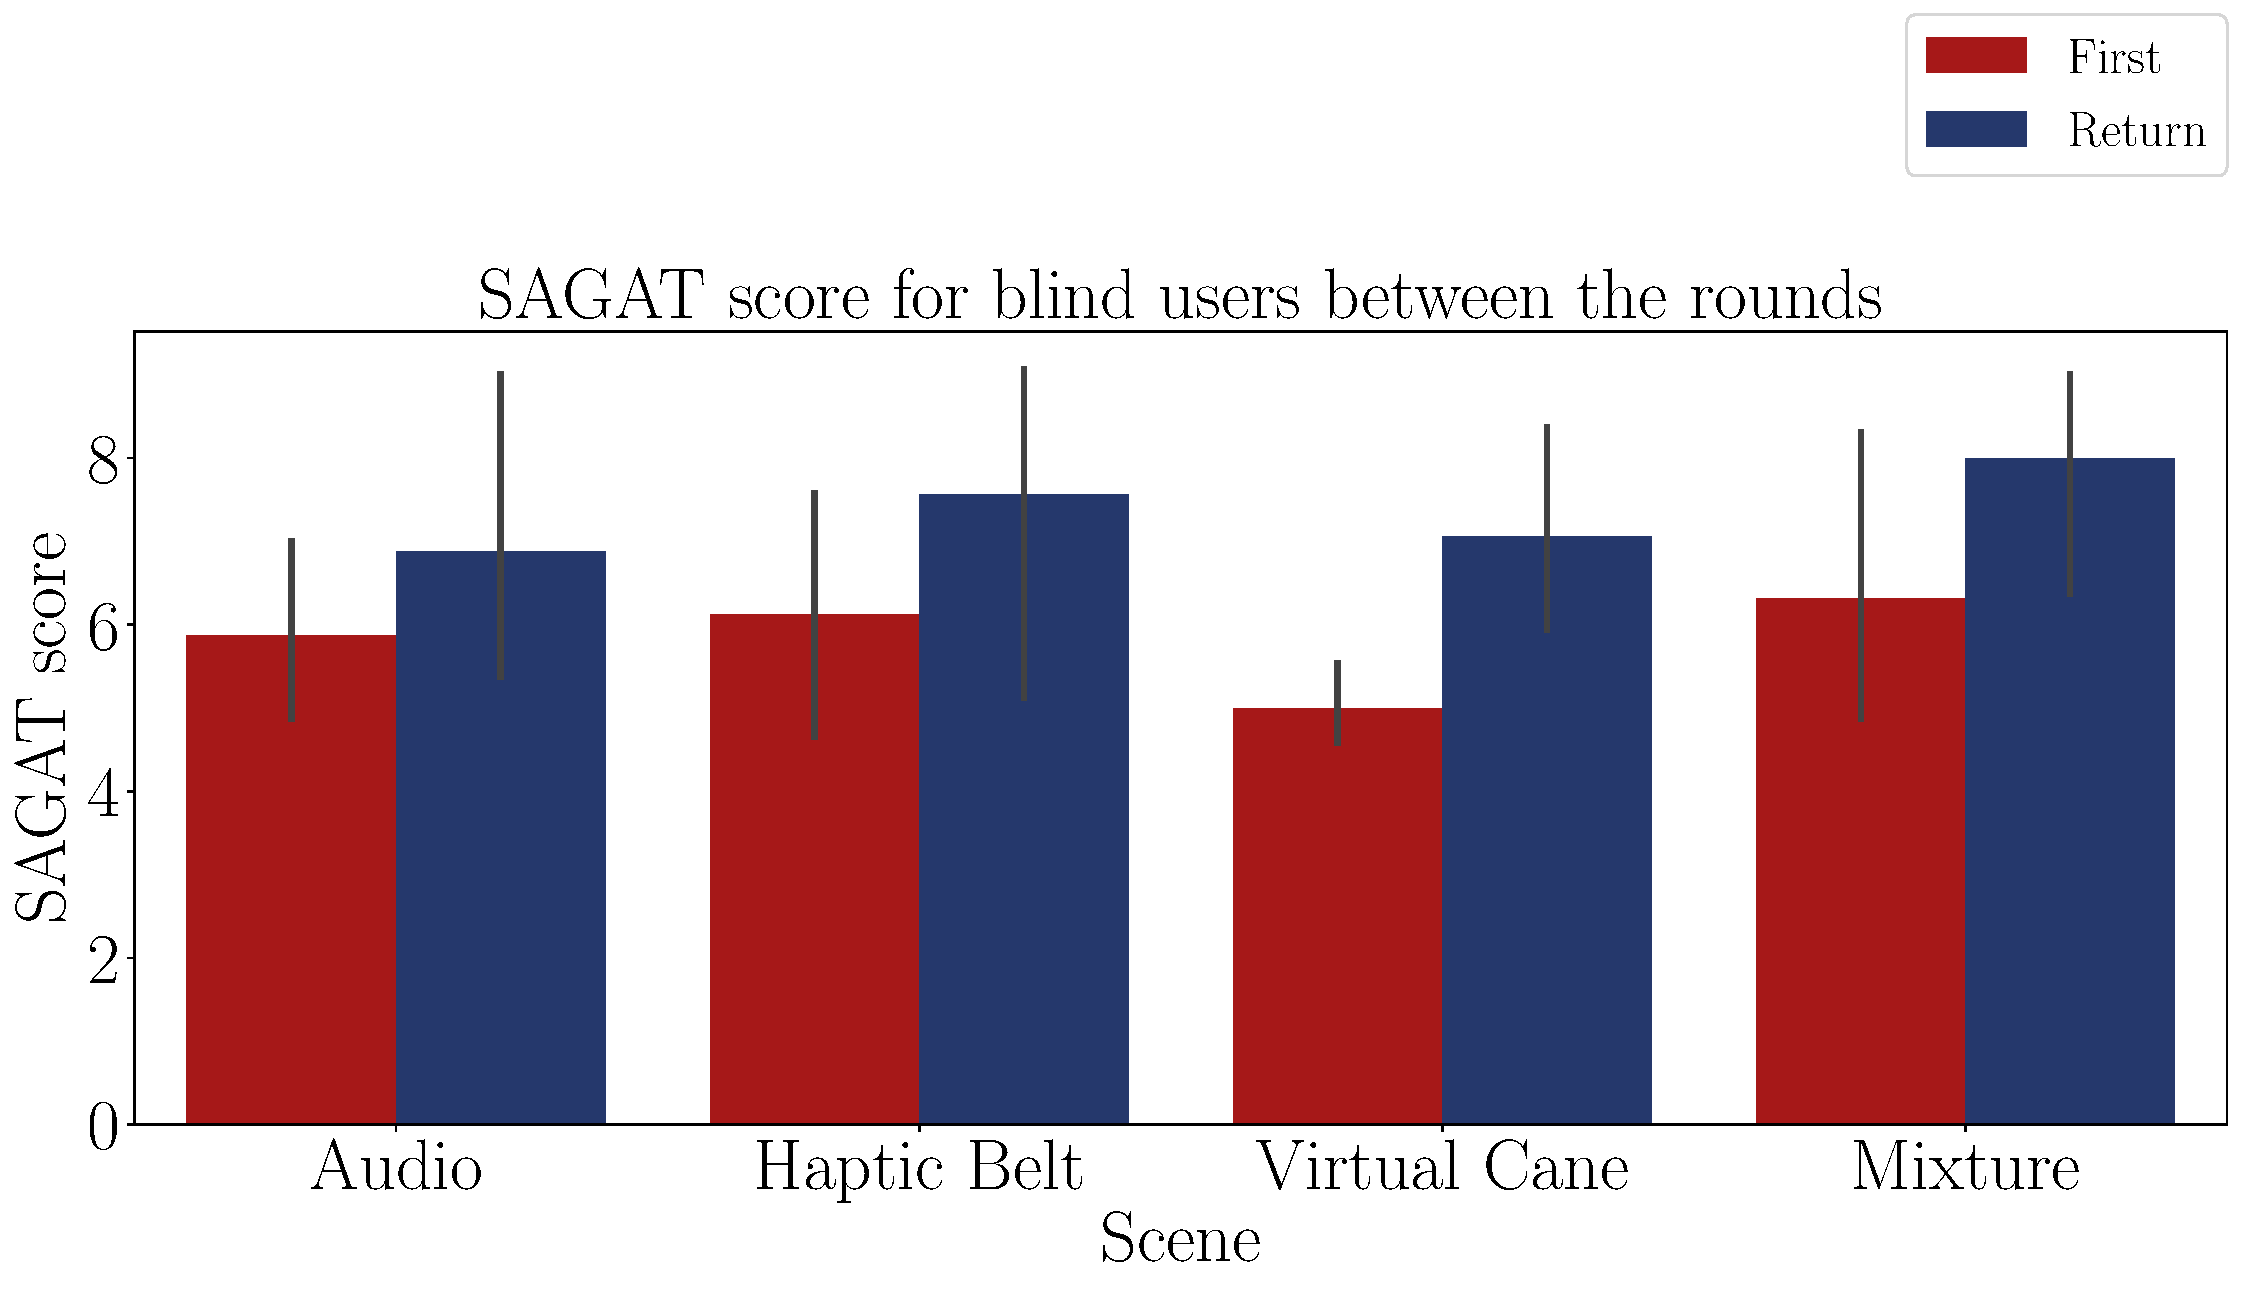
\includegraphics[width = \linewidth]{Resultados/Sagat/Figuras/pdf/barplot_sagat_avg_4_scene_blind.pdf}
%        \subcaption{Blind participants.}
%        \label{fig:barplot_sagat_avg_4_scene_blind}
%    \end{minipage}
%    \begin{minipage}{\linewidth}
%        \centering
%        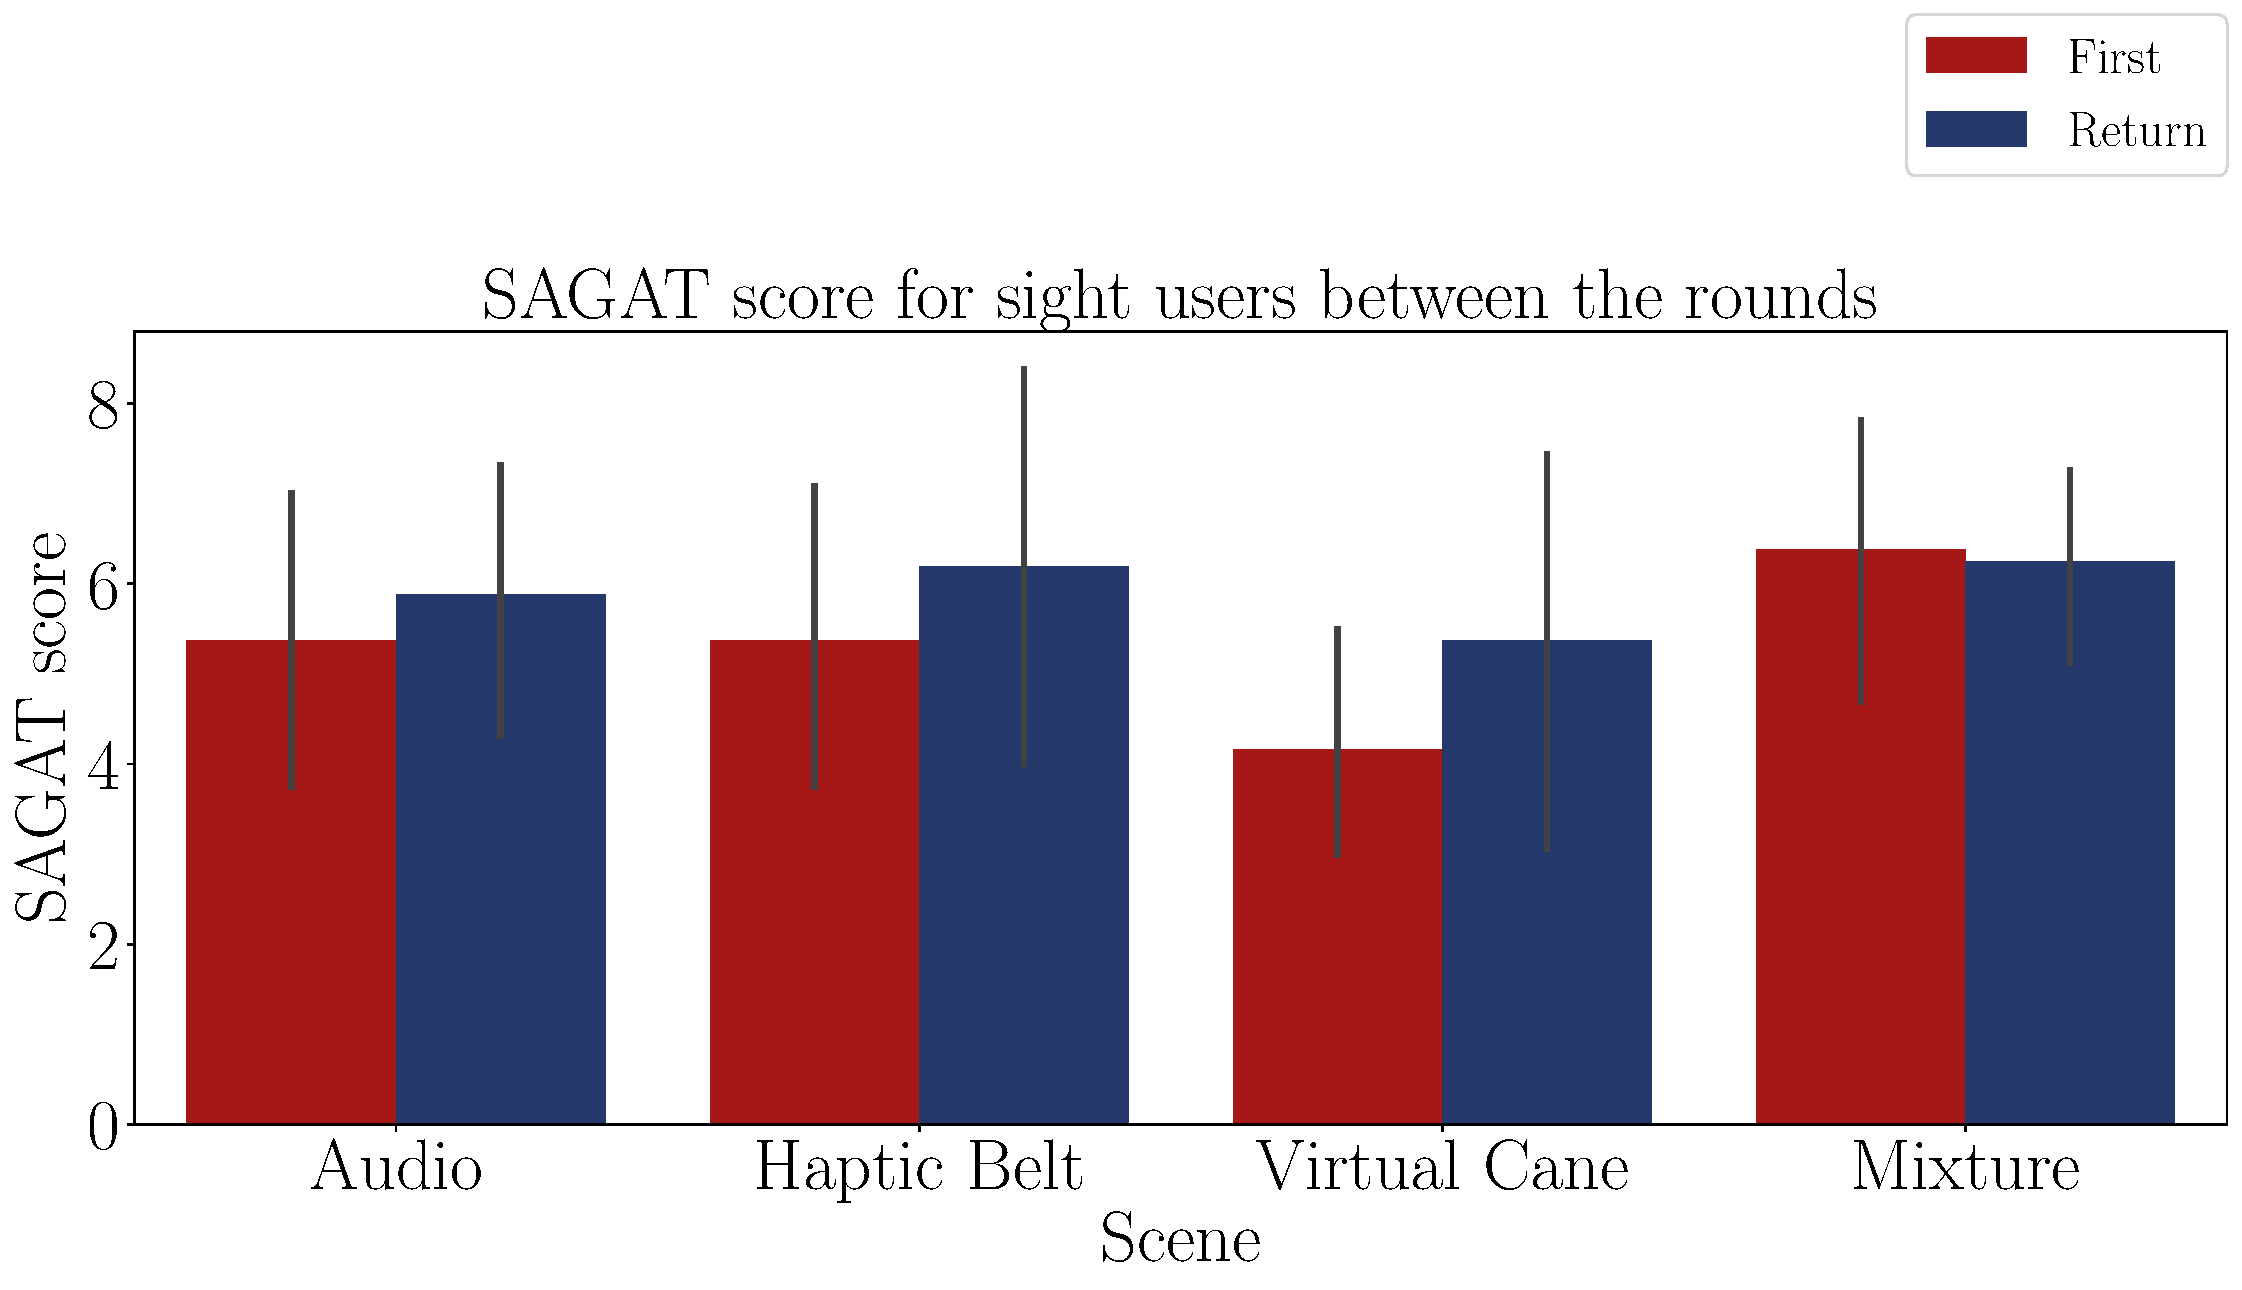
\includegraphics[width = \linewidth]{Resultados/Sagat/Figuras/pdf/barplot_sagat_avg_4_scene_sight.pdf}
%        \subcaption{Sight participants.}
%        \label{fig:barplot_sagat_avg_4_scene_sight}
%    \end{minipage}
%    \caption{Barplot of the SAGAT score on each method and each round.}
%    \label{fig:barplot_sagat_avg_4_scene_blind_sight}
%\end{figure}

Figures \ref{fig:boxplot_sagat_4_scene} and \ref{fig:boxplot_sagat_4_rounds} bring the boxplots. According to Figure \ref{fig:boxplot_sagat_4_scene}, both groups presented a higher situation awareness with ‘mixture’ and ‘haptic’. On the other hand, Figure \ref{fig:boxplot_sagat_4_rounds} confirms that the difference between the rounds is more significant for blind participants. 

\begin{figure}[!htb]
    \centering
    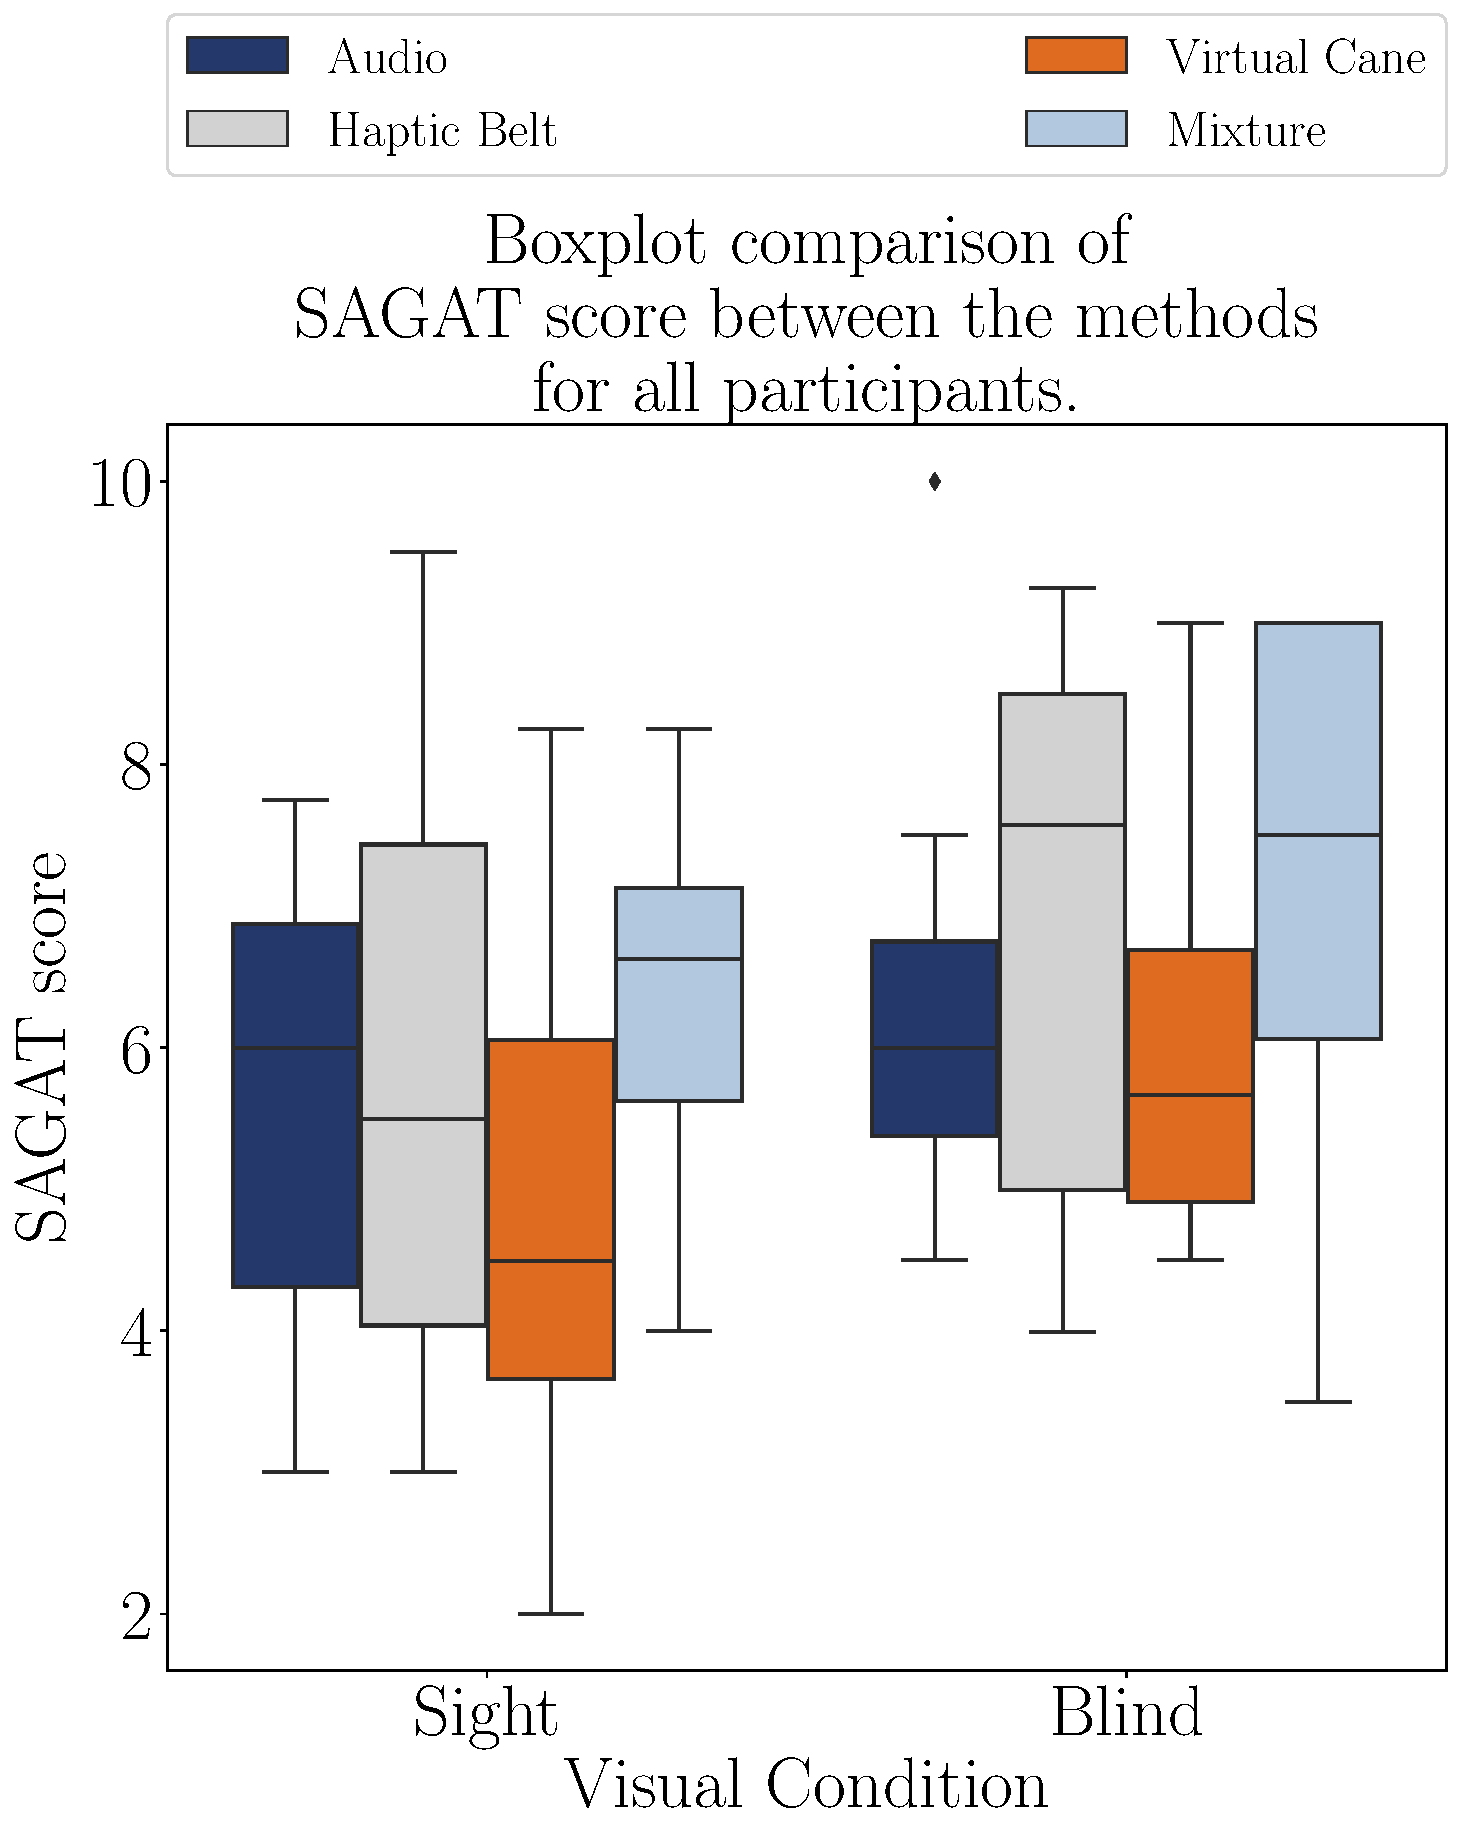
\includegraphics[width = 0.75\linewidth]{Resultados/Sagat/Figuras/pdf/boxplot_sagat_4_scene.pdf}
    \caption{Boxplot of the Sagat score of the participants grouped by the methods.}
    \label{fig:boxplot_sagat_4_scene}
\end{figure}
\begin{figure}[!htb]
    \centering
    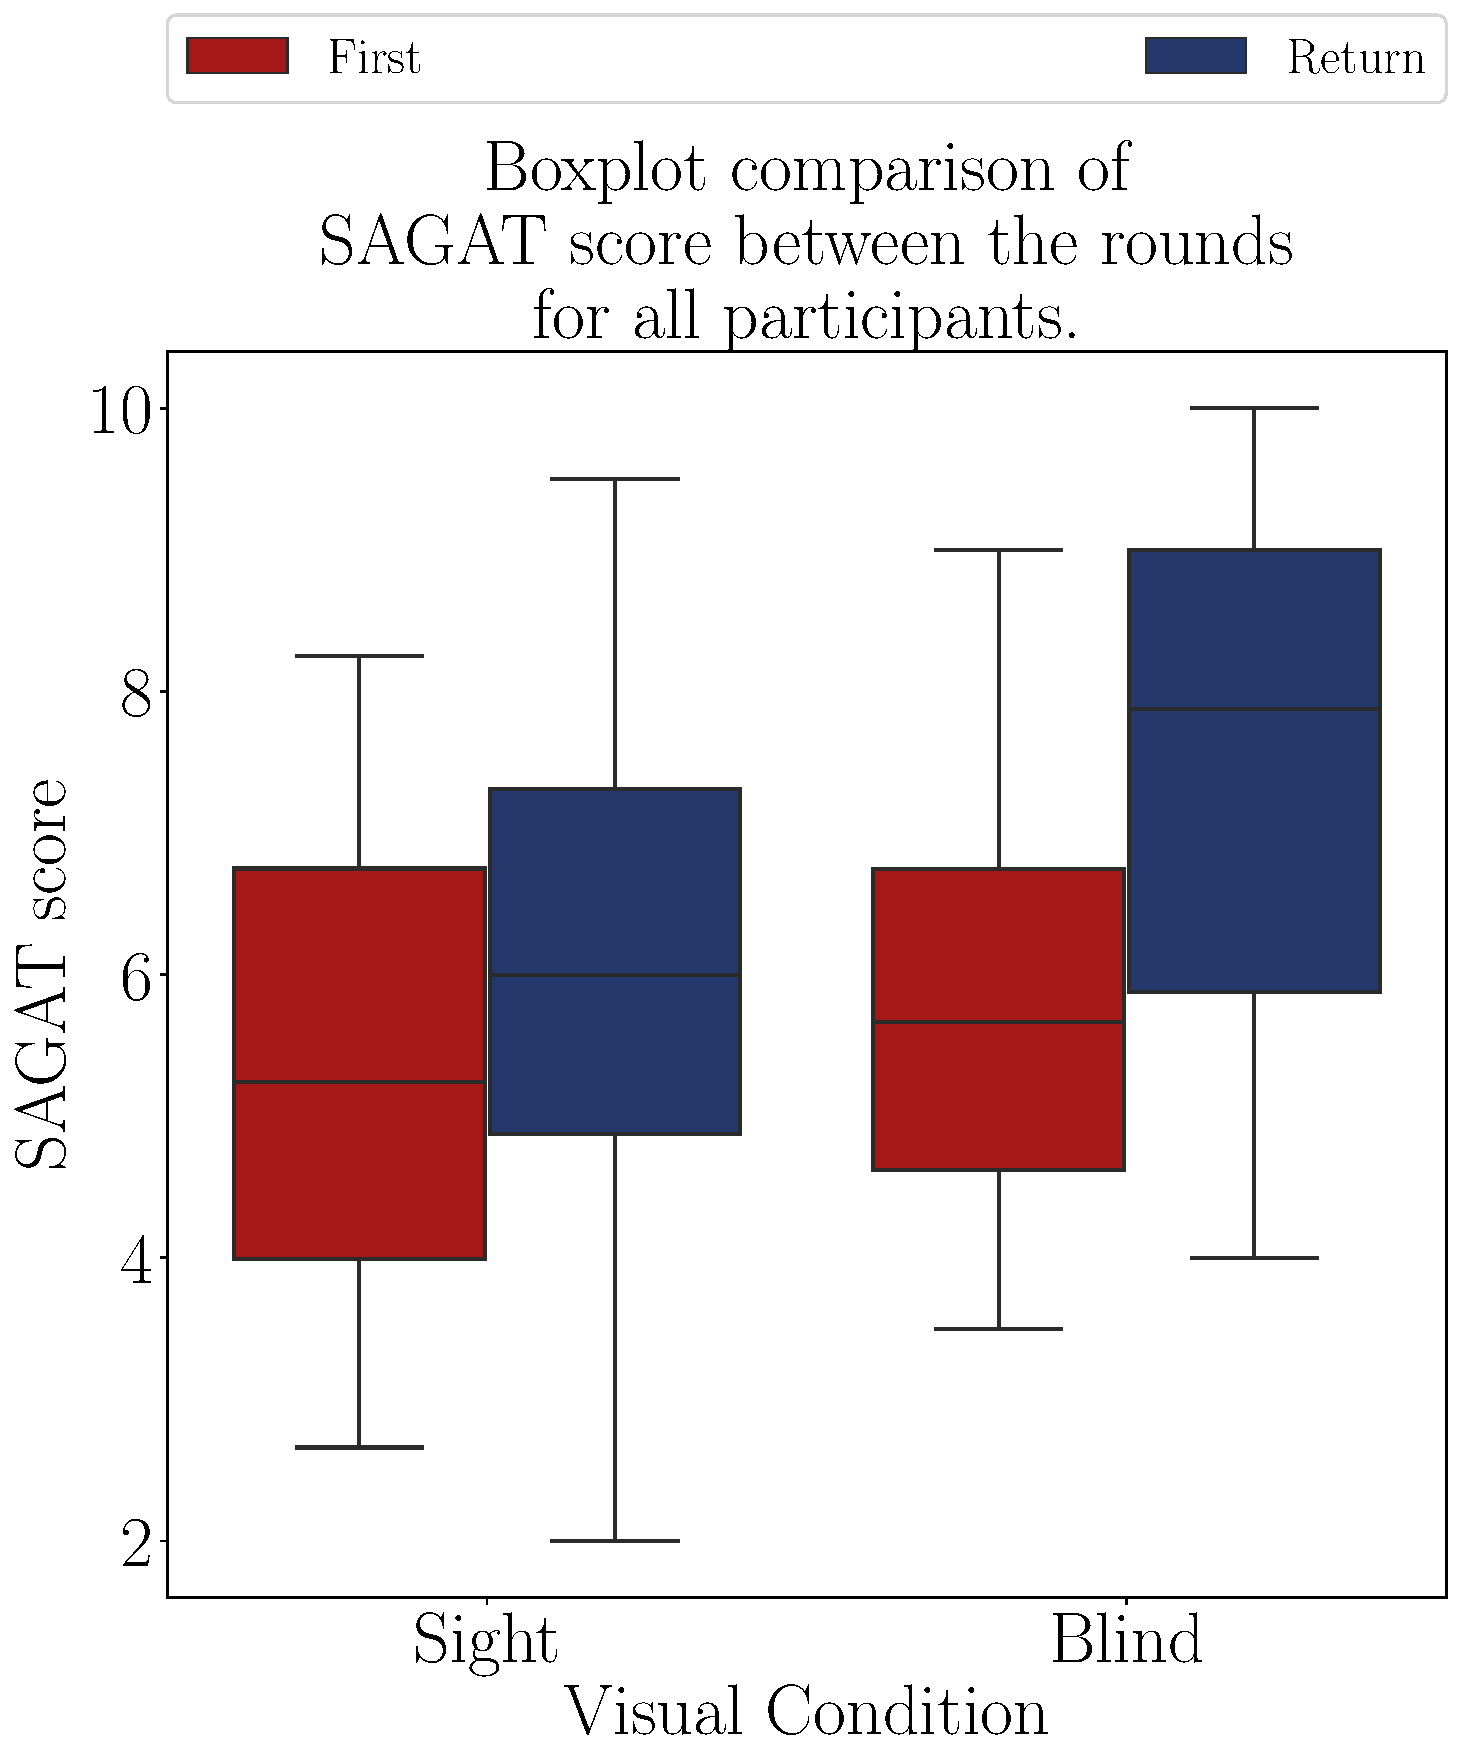
\includegraphics[width = 0.75\linewidth]{Resultados/Sagat/Figuras/pdf/boxplot_sagat_4_rounds.pdf}
    \caption{Boxplot of the Sagat score of the participants grouped by the rounds.}
    \label{fig:boxplot_sagat_4_rounds}
\end{figure}

%Figures \ref{fig:qqplot_sagat_avg_two_way_sight} and \ref{fig:residplot_sagat_avg_two_way_sight} brings the QQ plot and residual distribution. 
The variance of the residuals is not equal among the participants. Table \ref{tab:blocanova_sagat_avg_two_way_blind_sight} brings the p-value from ANOVA. While for the blind participants, the rounds are a significant factor and the methods are not, for the sighted participants the result is the opposite, showing a significant influence of the methods and not of the rounds.

\begin{table}[!htb]
    \caption{Anova p-value for the SAGAT score on each method}
    \label{tab:blocanova_sagat_avg_two_way_blind_sight}
\begin{minipage}{0.45\linewidth}
    \subcaption{Blind participants}
    \input{Resultados/Sagat/Tabelas/blocanova_sagat_avg_two_way_blindSemBegin.tex}
\end{minipage}%
\begin{minipage}{0.05\linewidth}
    \hfill
\end{minipage}%
\begin{minipage}{0.45\linewidth}
    \subcaption{Sight participants}
    \input{Resultados/Sagat/Tabelas/blocanova_sagat_avg_two_way_sightSemBegin.tex}    
\end{minipage}
\end{table}


%\begin{figure}[!htb]
%    \centering
%    %\vspace{-15.0cm}
%    \begin{minipage}{0.45\linewidth}
%        \centering
%        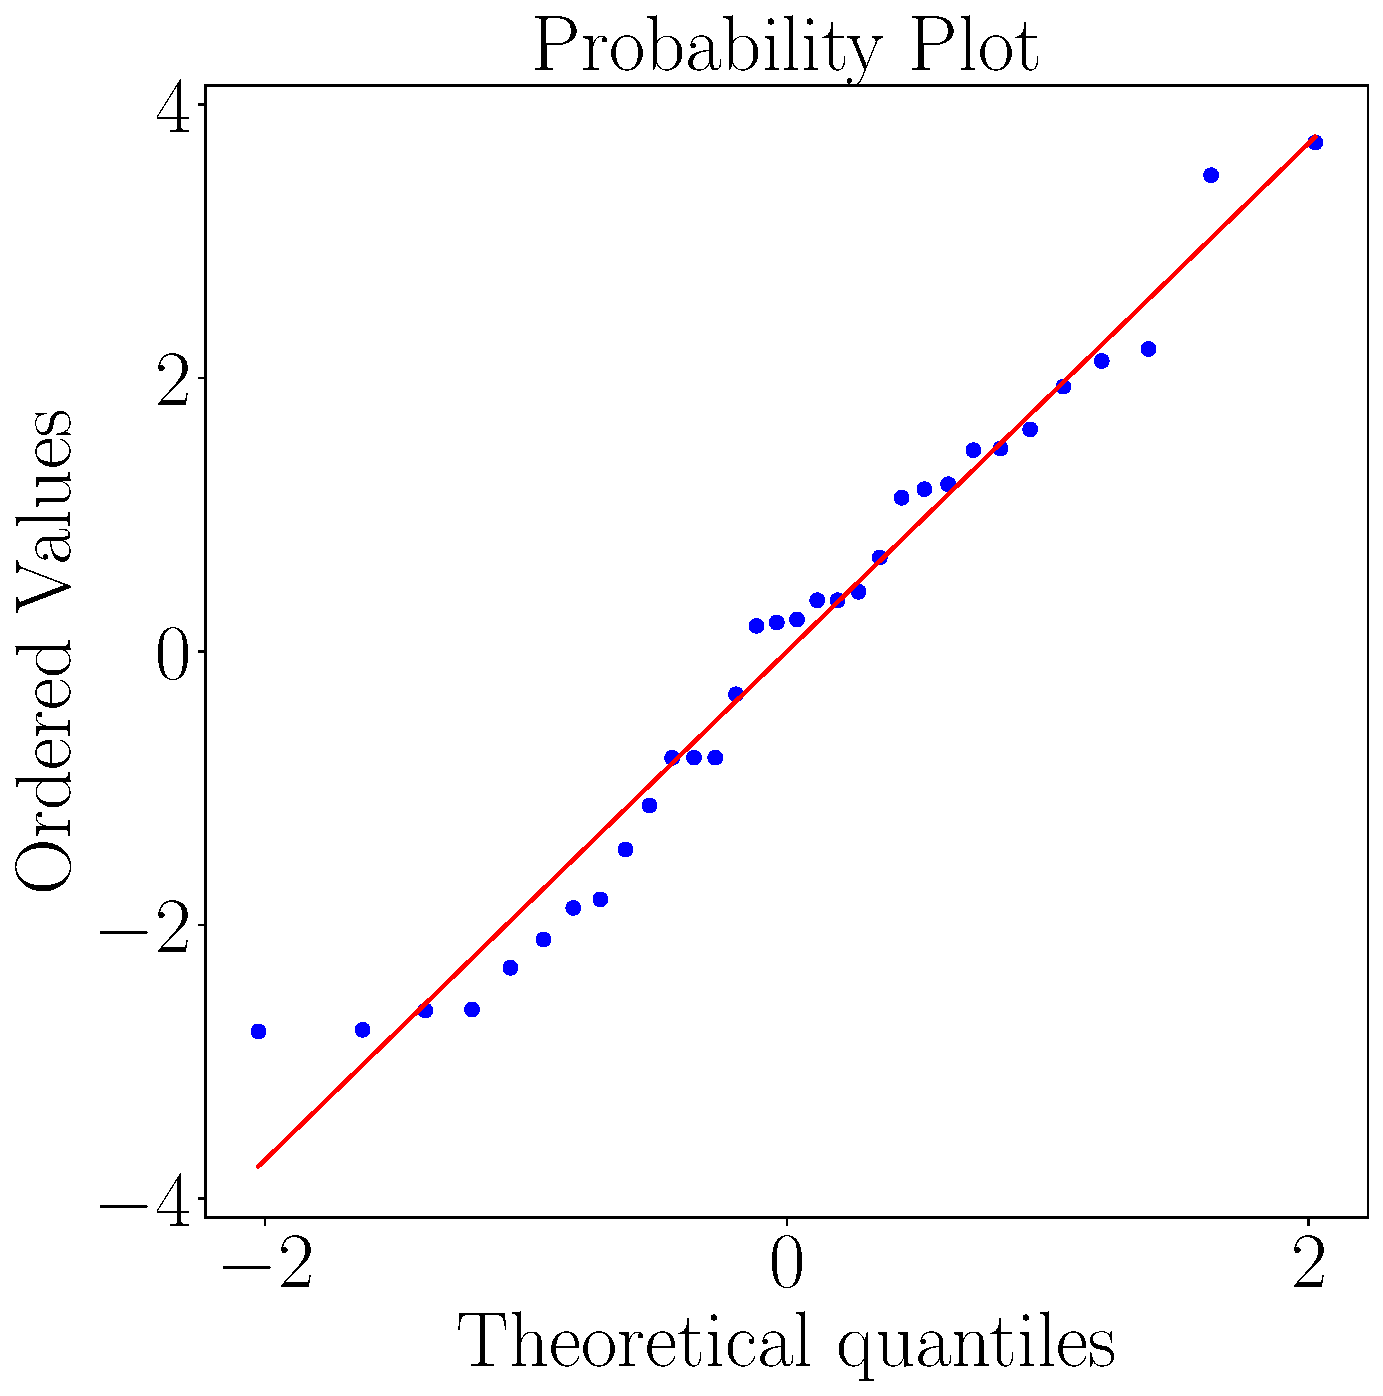
\includegraphics[width = \linewidth]{Resultados/Sagat/Figuras/pdf/qqplot_sagat_avg_two_way_sight.pdf}
%        \caption{QQ plot of the mental demand of the sight participants on each method.}
%        \label{fig:qqplot_sagat_avg_two_way_sight}
%    \end{minipage}
%    \begin{minipage}{0.075\linewidth}
%        \hfill
%    \end{minipage}
%    \begin{minipage}{0.45\linewidth}
%        \centering
%        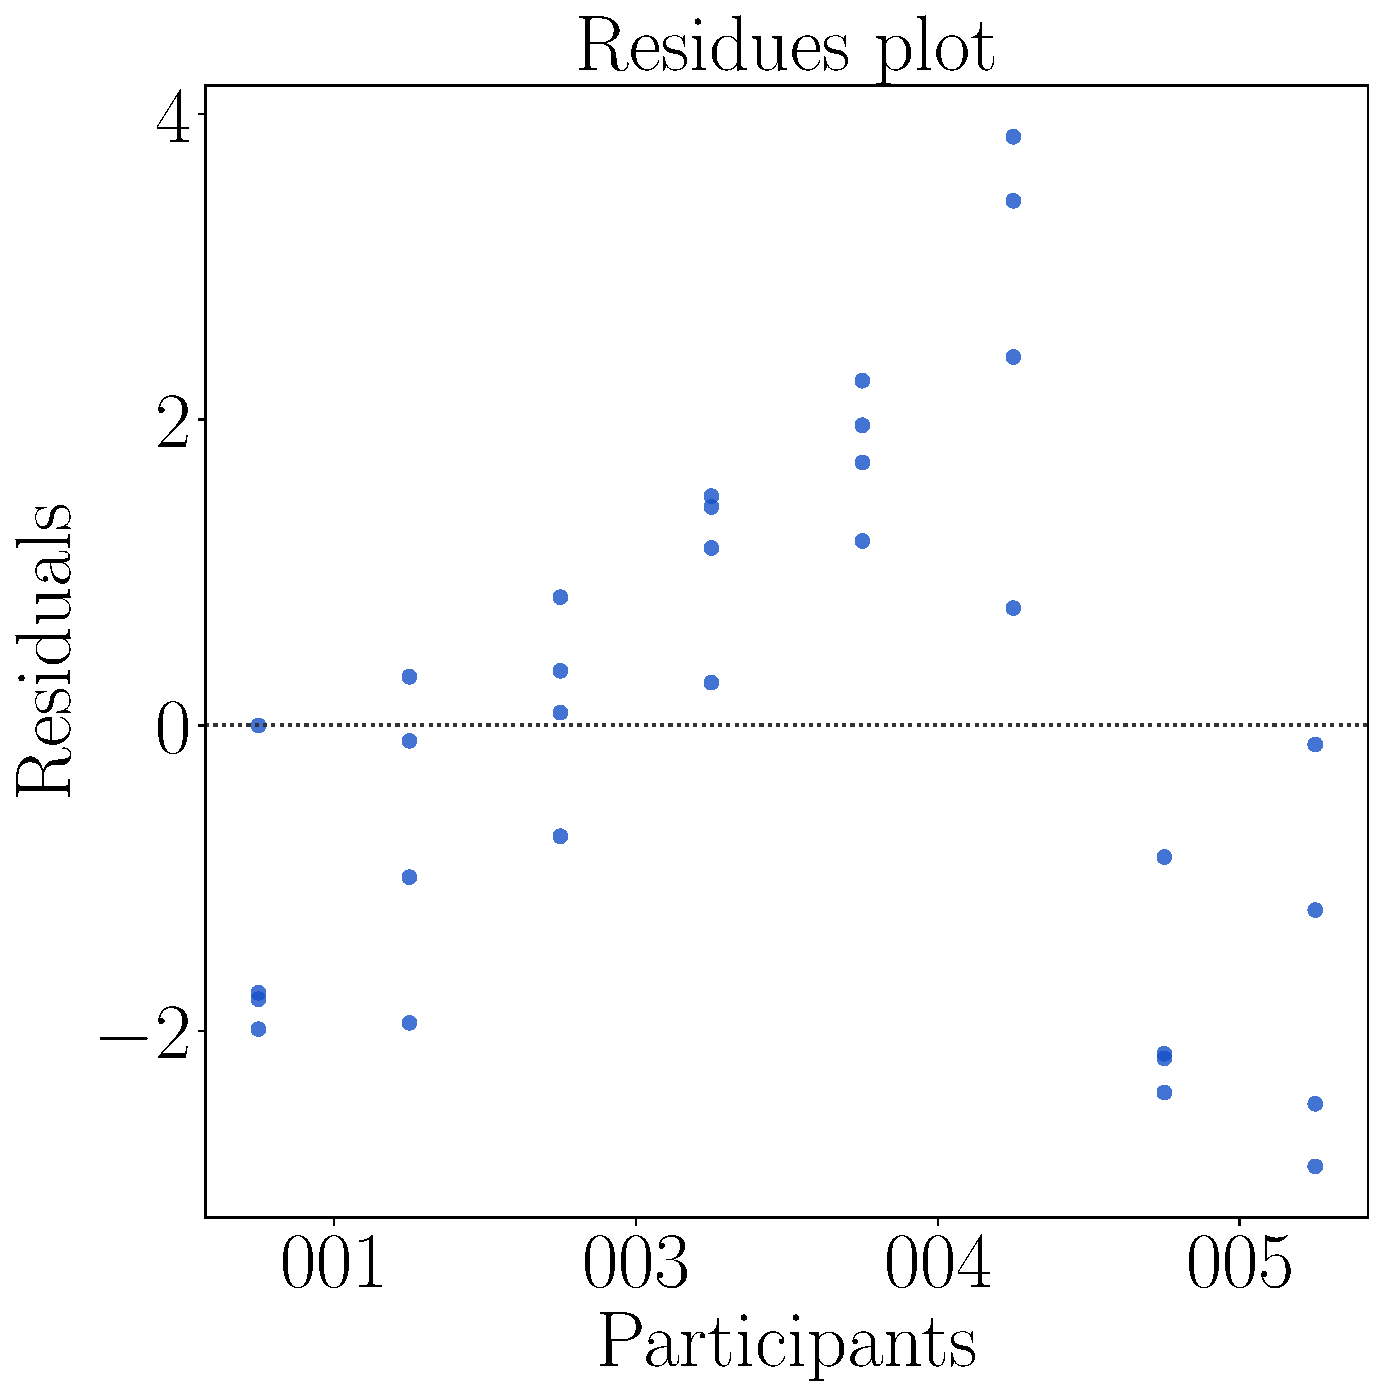
\includegraphics[width = \linewidth]{Resultados/Sagat/Figuras/pdf/residplot_sagat_avg_two_way_sight.pdf}
%        \caption{Residual plot of the mental demand score the sight participants on each method.}
%        \label{fig:residplot_sagat_avg_two_way_sight}
%    \end{minipage}
%\end{figure}
%
%%%%%%%%%%%%%%%%%%%%%%%%%%%%%%%%%%%%%%%%%%%%%%%%%%%%%%
%
%\FloatBarrier

\subsubsection{Guidance method's questionnaire.}
\label{subsubsec:results_questionnaires_2}

%As for the blind users, the sighted user also answered the Guidance questionnaire to give their thoughts about their experience with the guidance methods. Table \ref{tab:questionnaire_average} shows the score of both groups. As said before, the higher the value, the higher is the user satisfaction. The corresponding barplots are presented in Figure \ref{fig:barplot_questionnaire_scene_blind_sight}. Both groups prefer audio  and mixture methods. The difference lies in the preference between the haptic belt and virtual cane. The blind users tend to prefer the first one, while the sighted users tend to prefer the last.

%\input{Resultados/Questionario/Tabelas/questionnaire_average.tex}

%\begin{figure}[!htb]
%    \centering
%    \begin{minipage}{\textwidth}
%        \centering
%        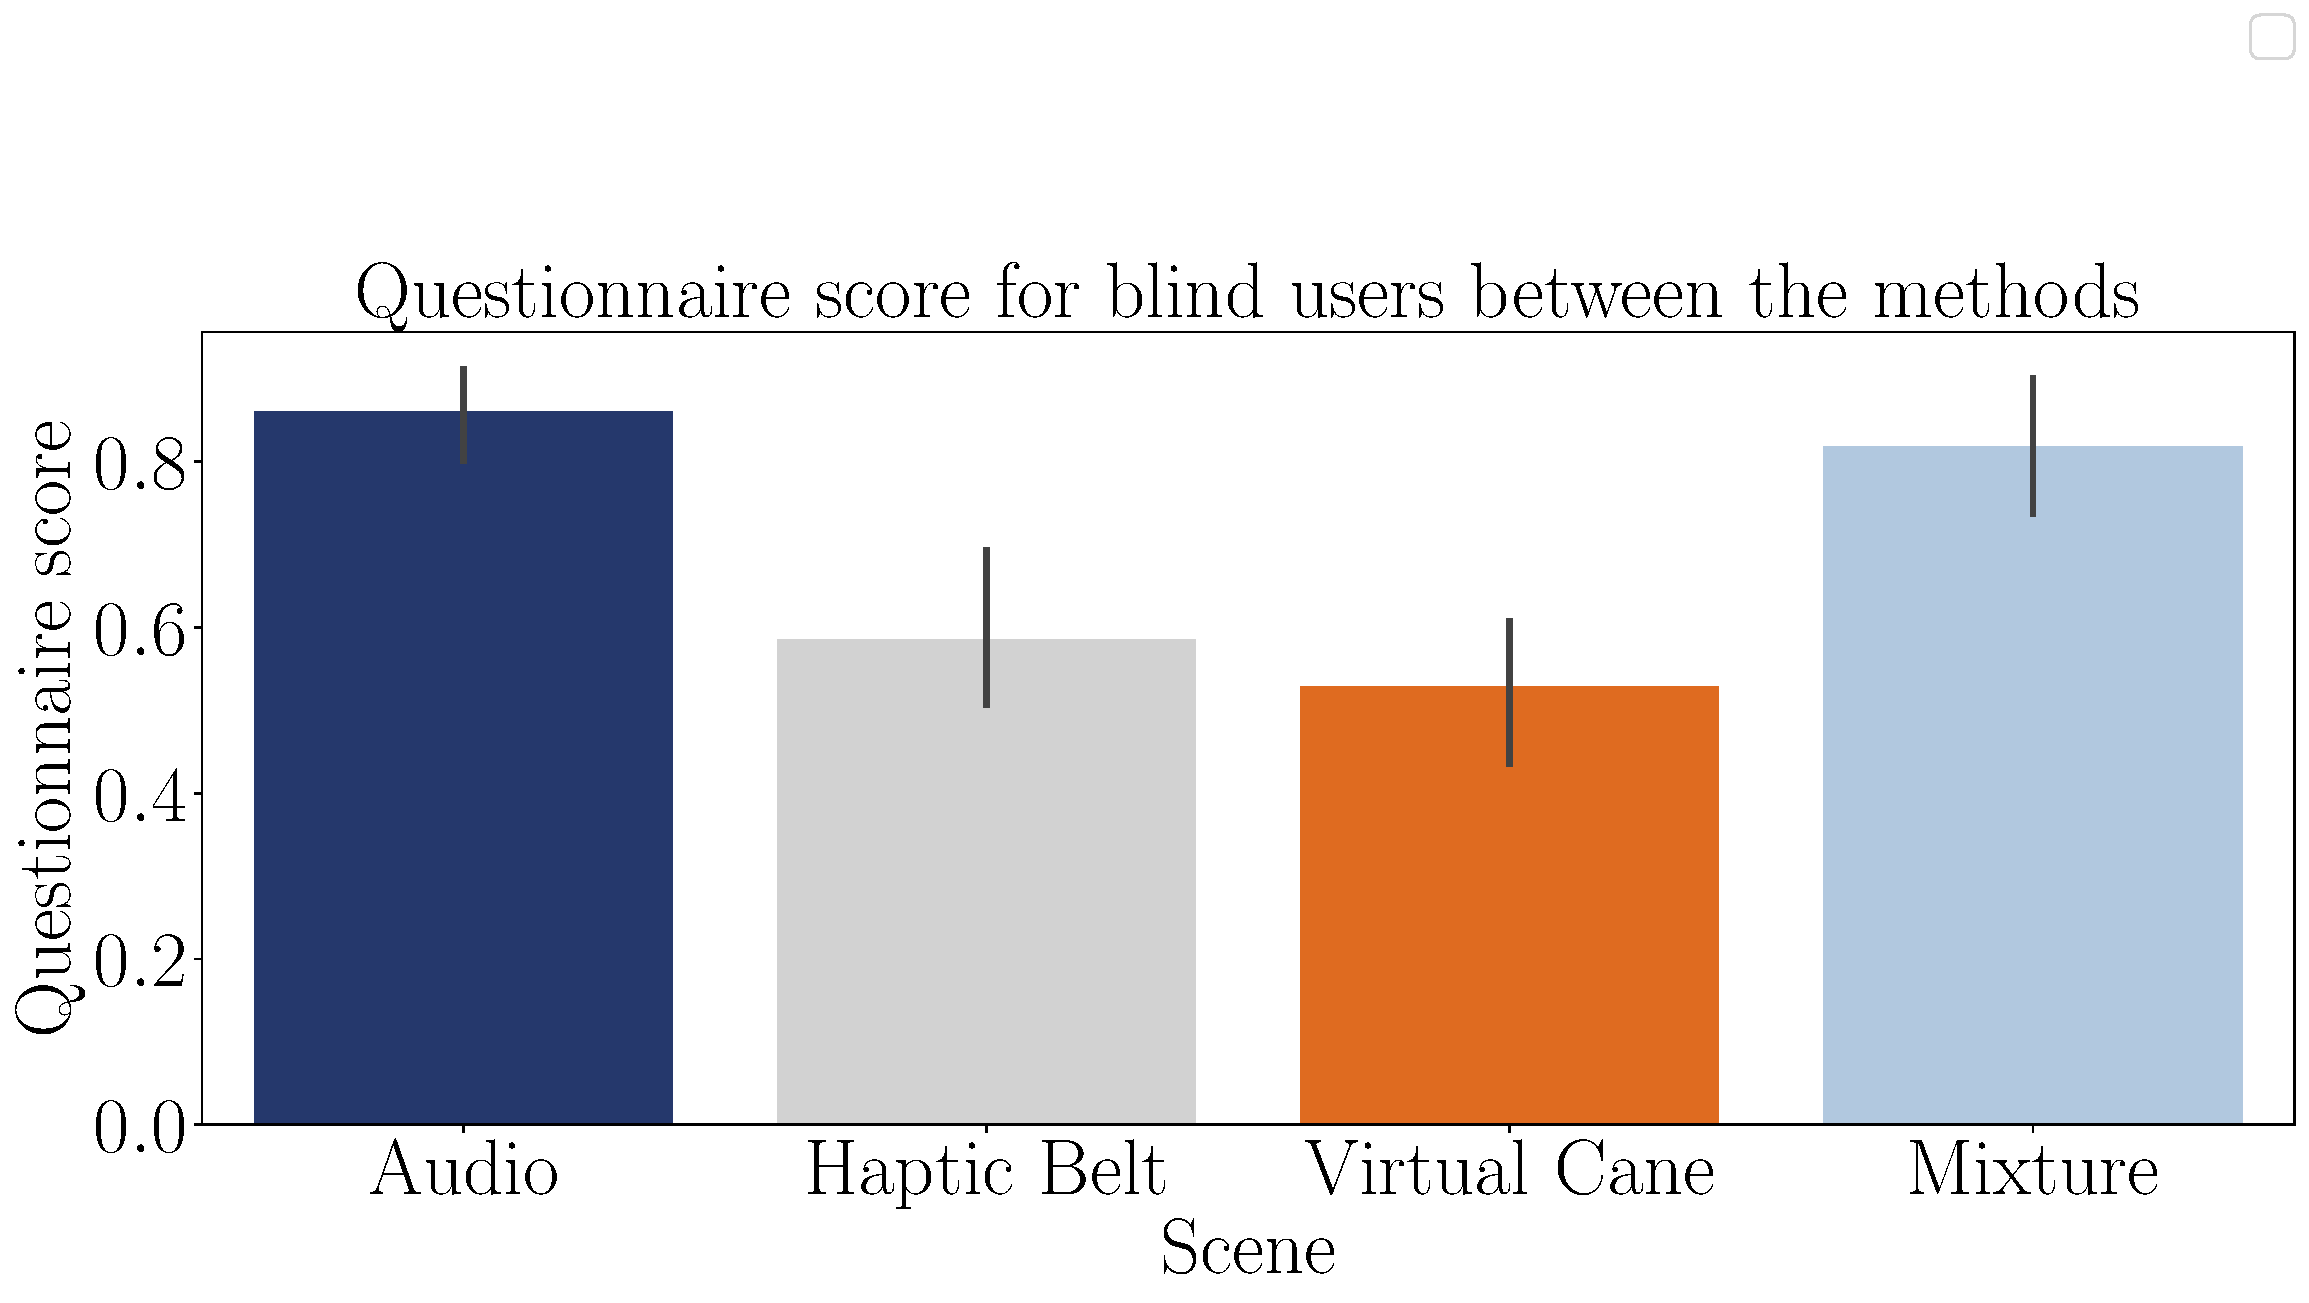
\includegraphics[width = \textwidth]{Resultados/Questionario/Figuras/pdf/barplot_questionnaire_scene_blind.pdf}
%        \subcaption{Blind participants.}
%        \label{fig:barplot_questionnaire_scene_blind_2}
%    \end{minipage}
%    \begin{minipage}{\textwidth}
%        \centering
%        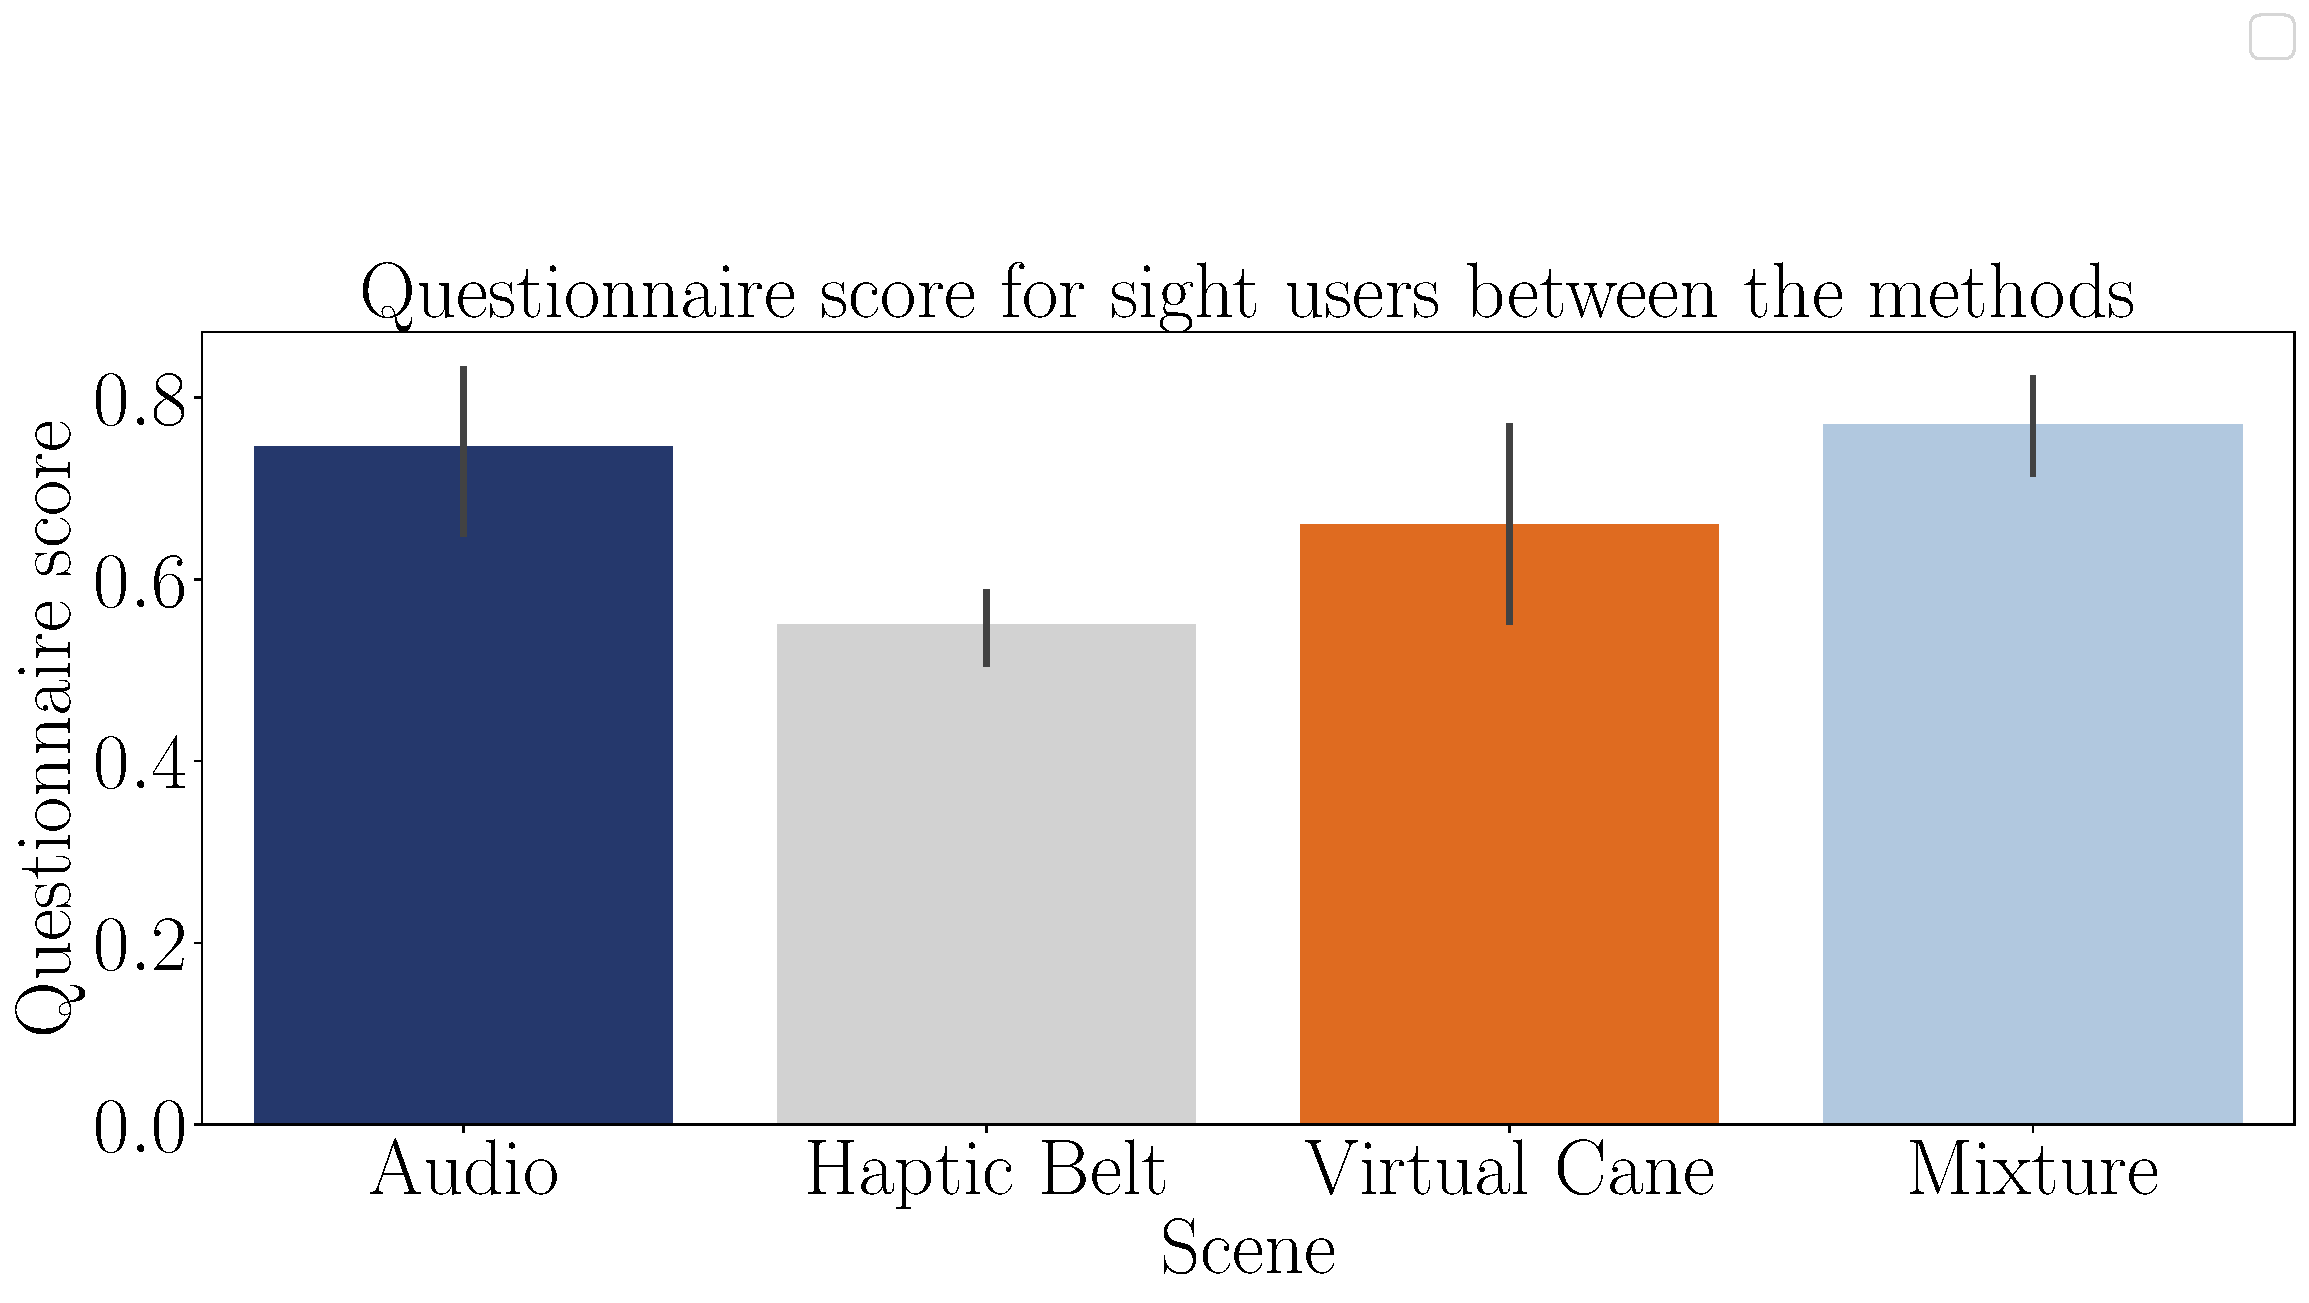
\includegraphics[width = \textwidth]{Resultados/Questionario/Figuras/pdf/barplot_questionnaire_scene_sight.pdf}
%        \subcaption{Sighted participants.}
%        \label{fig:barplot_questionnaire_scene_sight}
%    \end{minipage}
%    \caption{Barplot of the average questionaire score on each method.}
%    \label{fig:barplot_questionnaire_scene_blind_sight}
%\end{figure}
%\begin{figure}[!htb]
%    \centering
%    \includegraphics[width = \textwidth]{Resultados/Questionario/Figuras/png/barplot_questionnaire_scene.png}
%    \caption{Barplot of the  average questionaire score of both participants on each method.}
%    \label{fig:barplot_questionnaire_scene}
%\end{figure}

The Figure \ref{fig:boxplot_questionnaire_scene} presents the box plot with the distribution of the scores. It is possible to see that there is some similarity between the two groups, except for the virtual cane method, which has a broader distribution for the sighted users. Also, it seems that the audio and mixture have similar acceptance for sighted and blind users.

\begin{figure}[!htb]
    \centering
    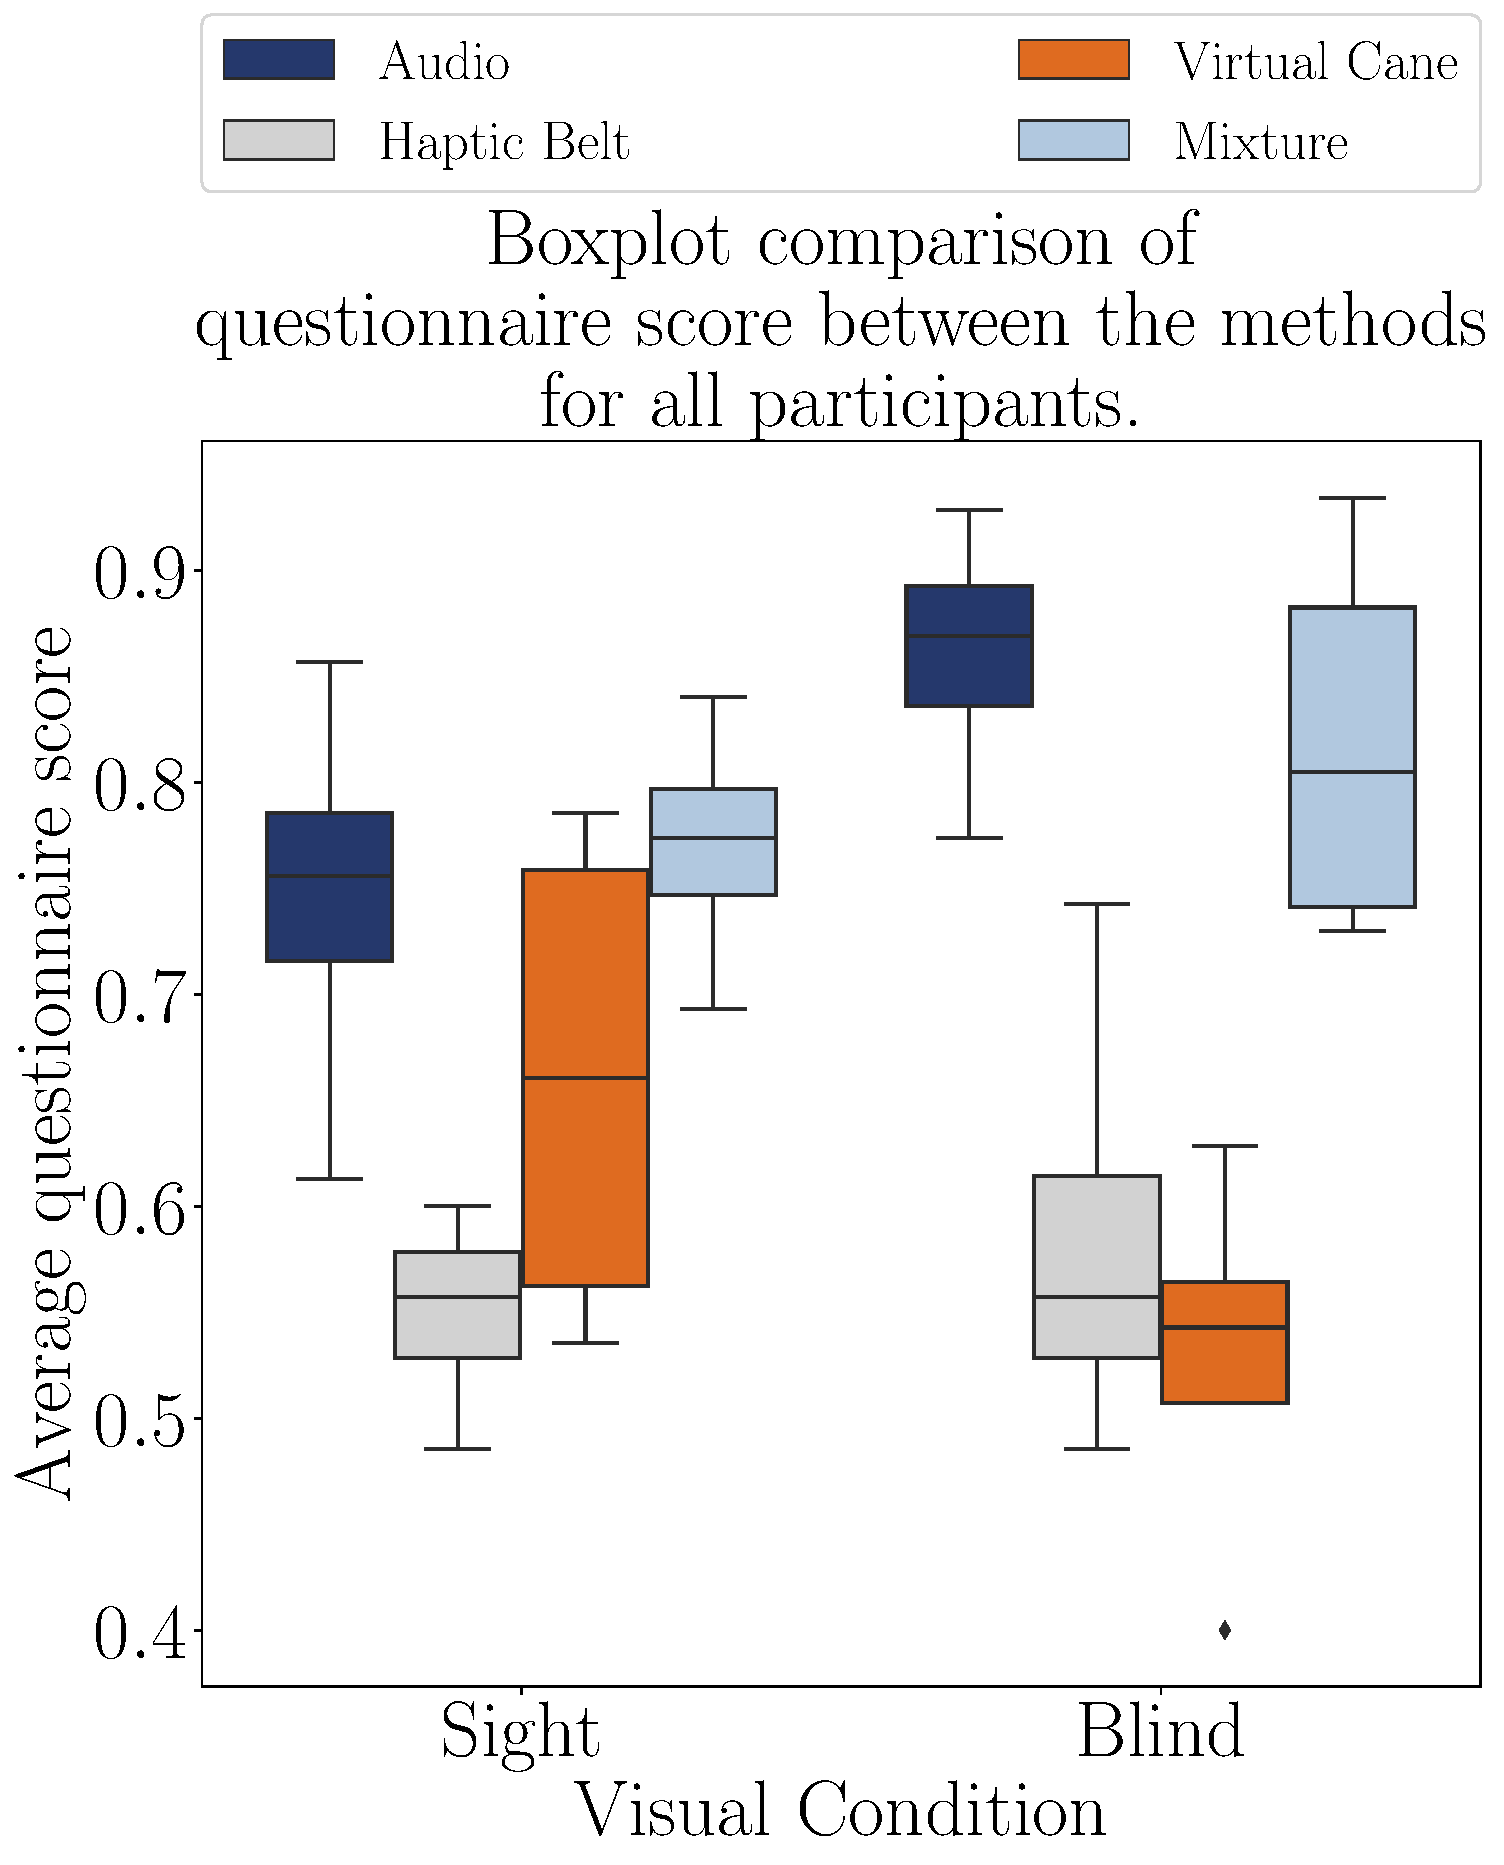
\includegraphics[width = 0.75\linewidth]{Resultados/Questionario/Figuras/pdf/boxplot_questionnaire_scene.pdf}
    \caption{Boxplot of the questionaire score of the the participants grouped by the methods.}
    \label{fig:boxplot_questionnaire_scene}
\end{figure}

%The Table \ref{tab:questionnaire_average_group} show the the average questionnaire score on each method of both groups and it shows the same conclusion as the Figure \ref{fig:barplot_questionnaire_scene}, that the preference between the "Haptic Belt" and "Virtual Cane" is the only difference between the two groups.
%
%Considering the most preferable and the less preferable of each group, the blind users are score their choices more intesiver than the sighted users. This may be an effect from their previous experience with the "Audio" method in previous events before the experiment and with haptic devices were something very, or almost, new. For the sighted users everything was new, so there scores were more consistent. This is posible to see in the average and standar deviation of these scores. For the blind users is 0.7 and 0.164 and for the sighted user is 0.682 and 0.100.
%
%\input{Resultados/Questionario/Tabelas/questionnaire_average_group}

%Figures \ref{fig:qqplot_questionnaire_sight} and \ref{fig:residplot_questionnaire_sight} brings the QQ plot and residual distribution, which confirm that ANOVA can be applied.
The result of ANOVA is presented in Table \ref{tab:blocanova_questionnaire_blind_sight} and indicates that the method is an effective variable for the sighted participants, as it is for the blind ones.

\begin{table}[!htb]
    \caption{Anova p-value for the questionnaire score on each method}
    \label{tab:blocanova_questionnaire_blind_sight}
\begin{minipage}{0.45\linewidth}
    \subcaption{Blind participants.}
    \input{Resultados/Questionario/Tabelas/blocanova_questionnaire_blindSemBegin.tex}
\end{minipage}%
\begin{minipage}{0.05\linewidth}
\end{minipage}%
\begin{minipage}{0.45\linewidth}
    \subcaption{Sight participants.}
    \input{Resultados/Questionario/Tabelas/blocanova_questionnaire_sightSemBegin.tex}
\end{minipage}
\end{table}

%\begin{figure}[!htb]
%    \centering
%    %\vspace{-15.0cm}
%    \begin{minipage}{0.45\textwidth}
%        \centering
%        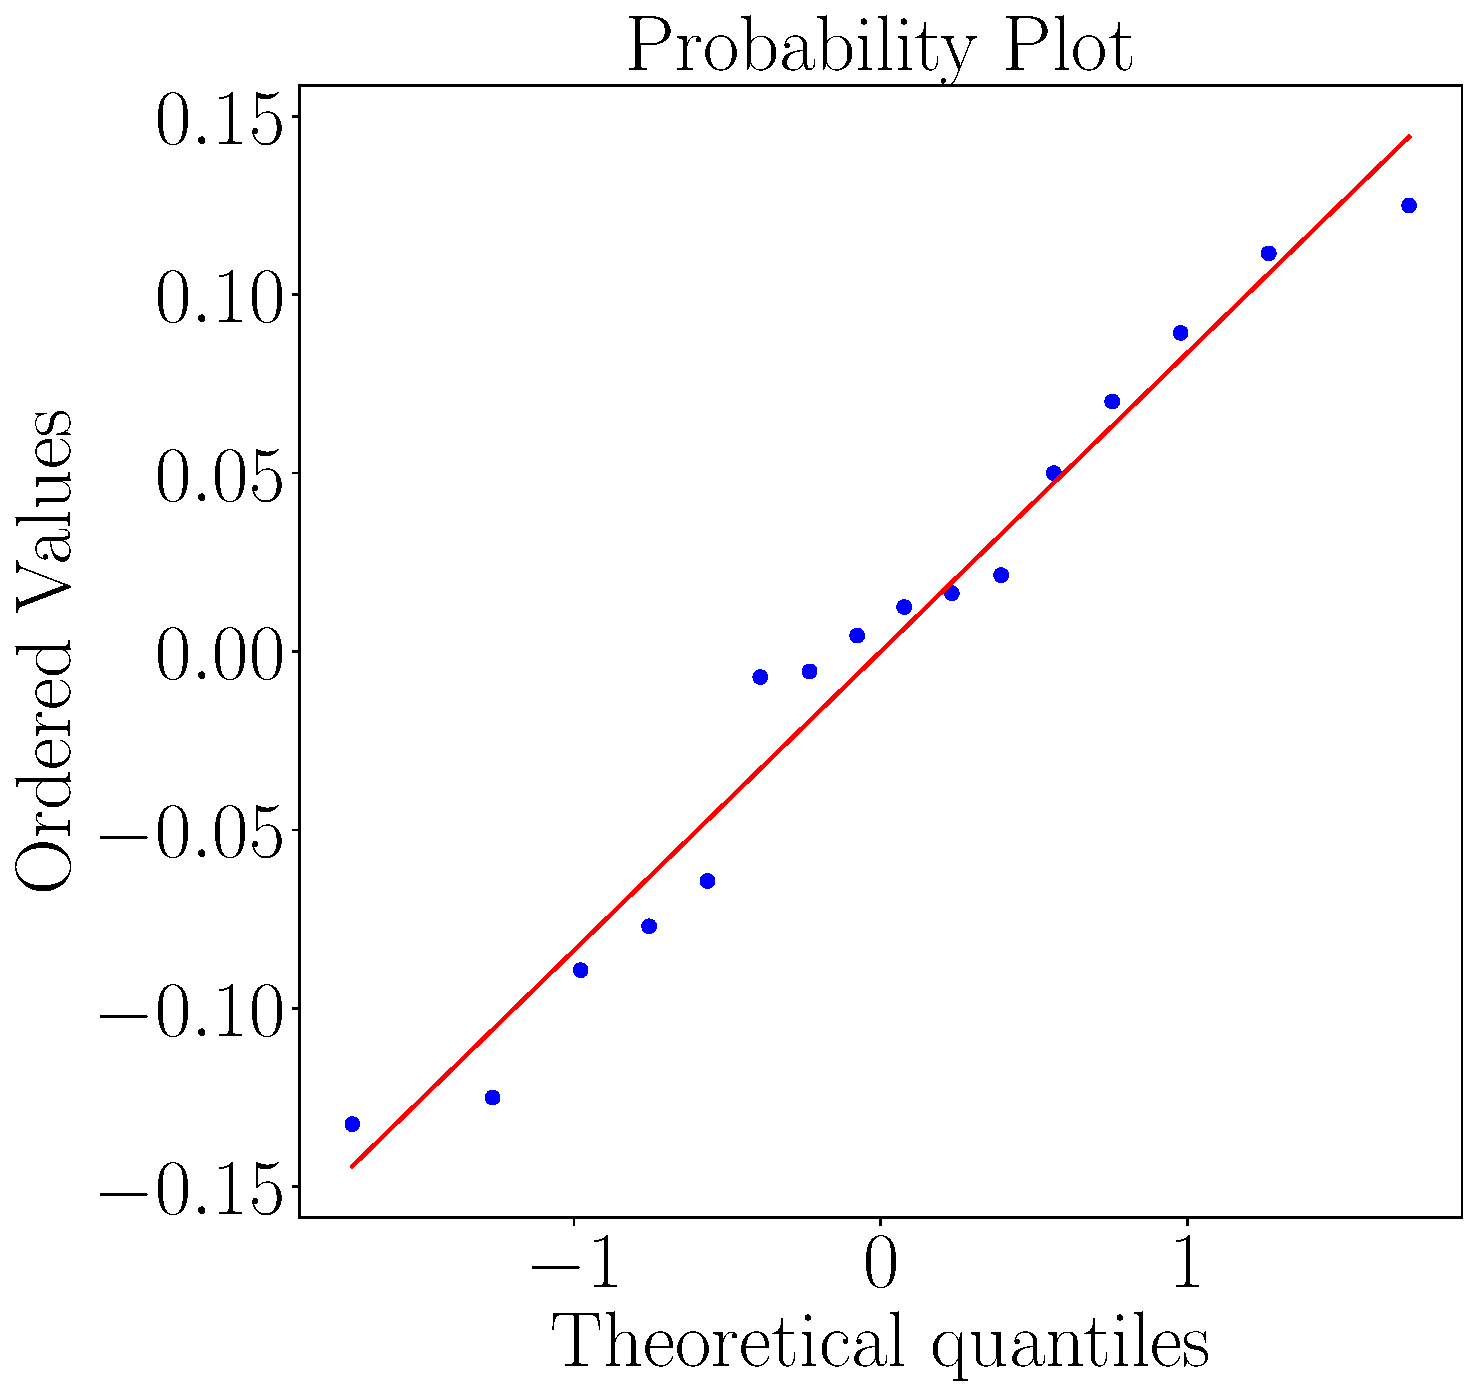
\includegraphics[width = \textwidth]{Resultados/Questionario/Figuras/pdf/qqplot_questionnaire_sight.pdf}
%        \caption{QQ plot of the questionnaire score of the sighted participants on each method.}
%        \label{fig:qqplot_questionnaire_sight}
%    \end{minipage}
%    \begin{minipage}{0.075\textwidth}
%        \hfill
%    \end{minipage}
%    \begin{minipage}{0.45\textwidth}
%        \centering
%        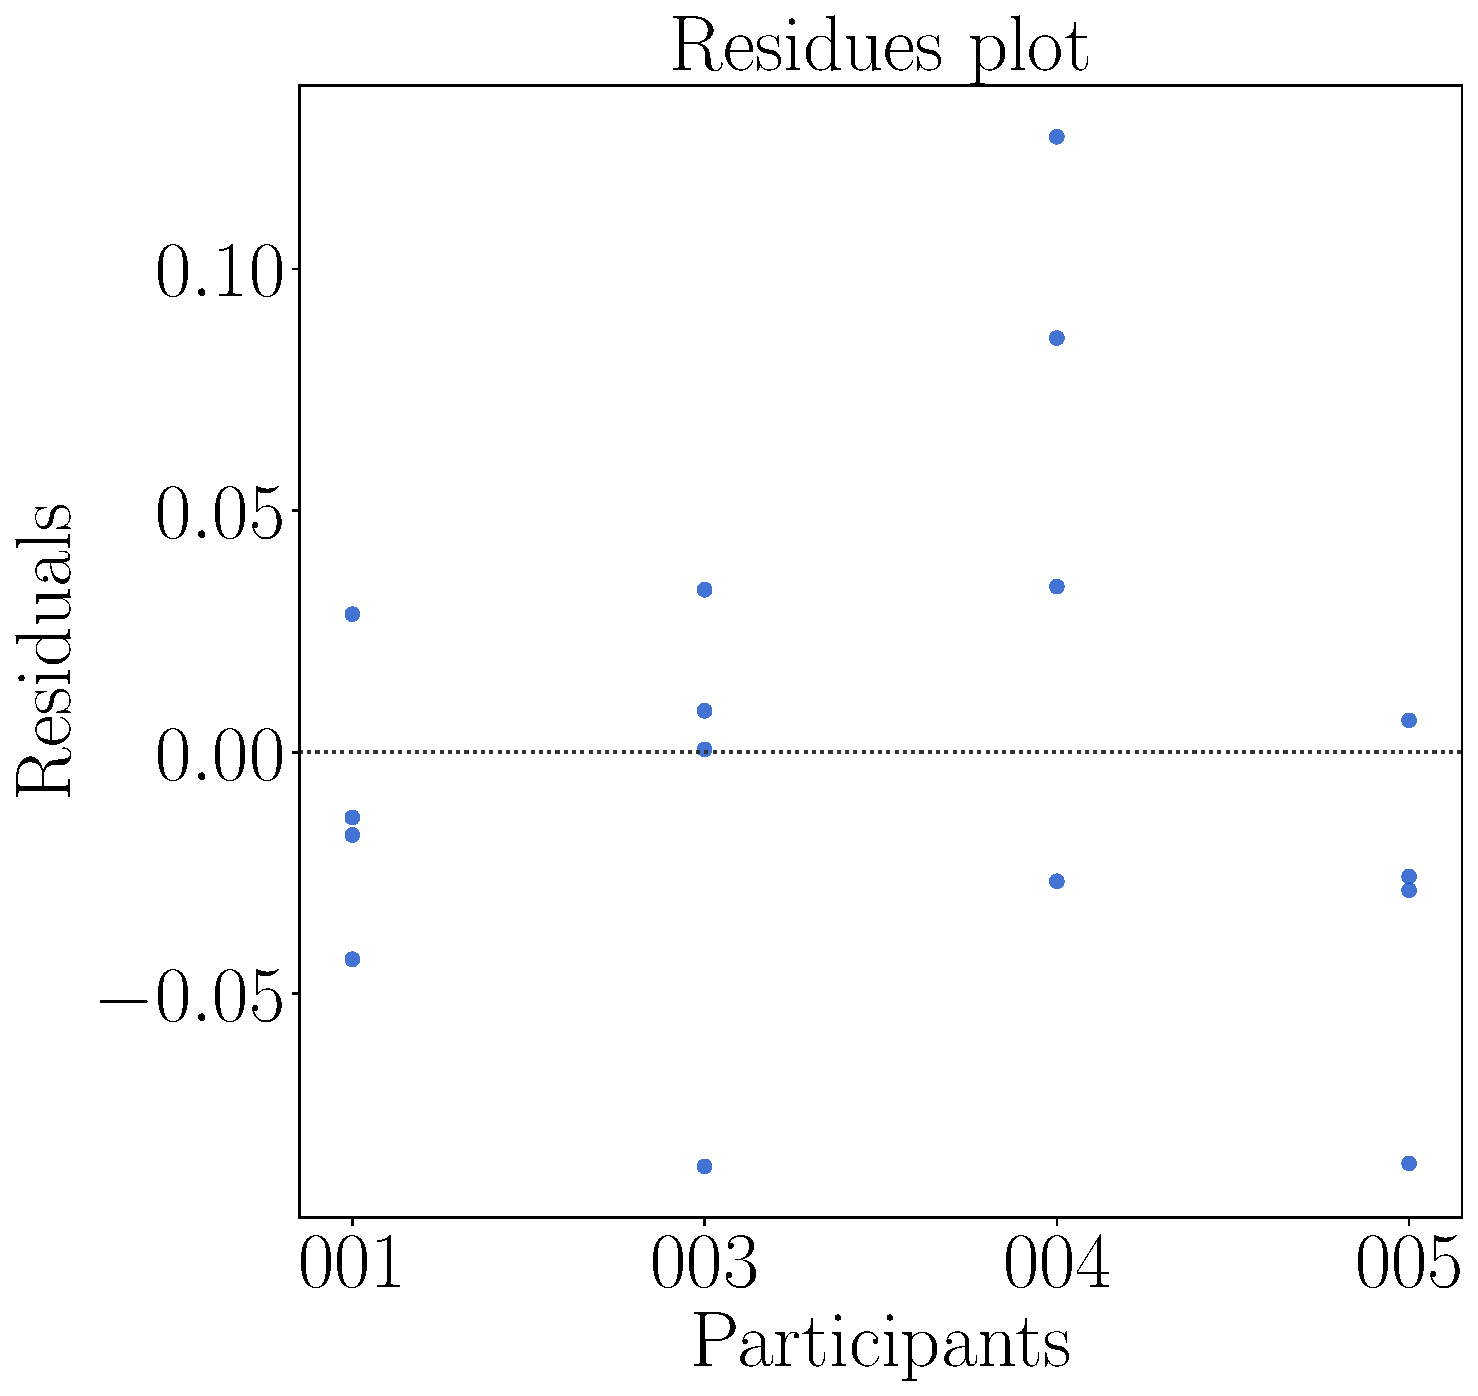
\includegraphics[width = \textwidth]{Resultados/Questionario/Figuras/pdf/residplot_questionnaire_sight.pdf}
%        \caption{Residual plot of the questionnaire score the sighted participants on each method.}
%        \label{fig:residplot_questionnaire_sight}
%    \end{minipage}
%\end{figure}
%
Table \ref{tab:lsd_questionnaire_blind_sight} presents the conclusion of 
A pairwise Fisher LSD test between all the guidance methods for both groups shows that the results are coincident between the two groups.

%\FloatBarrier

\begin{table*}[!thb]
    \caption{Anova p-value for the mental demand average on each method'}
    \label{tab:lsd_questionnaire_blind_sight}
    \begin{minipage}{1\textwidth}
        \subcaption{Blind participants.}
        \input{Resultados/Questionario/Tabelas/lsd_questionnaire_blindSemBegin.tex}
    \end{minipage}
    \begin{minipage}{1\textwidth}
        \subcaption{Sight participants.}
        \input{Resultados/Questionario/Tabelas/lsd_questionnaire_sightSemBegin.tex}
    \end{minipage}
\end{table*}

%\input{Resultados/Questionario/Tabelas/lsd_questionnaire.tex}

%The LSD Table \ref{tab:lsd_questionnaire_sight} repeat the same conclusion of the blind participants, that only the "Audio" and "Mixture" are statistically the same. But that does not mean that both groups had the same opinion from the rest of the methods. As shown in the Figure \ref{fig:boxplot_questionnaire_scene}, the average sighted user rather use the "Virtual Cane" then the "Haptic Belt", despite that distribution being wider, hence more varied, meaning that this is hardly a consense between the users.

%\FloatBarrier
%\subsection{Subjective data}
\subsubsection{NASA-TLX}
\label{subsubsec:results_nasa_tlx_2}

\paragraph*{Analysis of the mental demand scale}\mbox{}\\

Figures \ref{fig:boxplot_noBase_md_4_scene} and \ref{fig:boxplot_noBase_md_4_rounds} presents the box plot for both groups, organized by the methods and the rounds. The mental demand is systematically higher for sighted people, which is expected. However, while blind participants considered the audio method less demanding, sighted participants prefered to the virtual cane. For both groups, we observe a decrease in the mental demand.

\begin{figure}[!htb]
    \centering
    \includegraphics[width = 0.75\linewidth]{3 - Resultados/Figuras/boxplot_noBase_md_4_scene.pdf}
    \caption{Boxplot of the mental demand of the participants grouped by the methods.}
    \label{fig:boxplot_noBase_md_4_scene}
\end{figure}
\begin{figure}[!htb]
    \centering
    \includegraphics[width = 0.75\linewidth]{3 - Resultados/Figuras/boxplot_noBase_md_4_rounds.pdf}
    \caption{Boxplot of the mental demand of the participants grouped by the rounds.}
    \label{fig:boxplot_noBase_md_4_rounds}
\end{figure}

Table \ref{tab:blocanova_md_avg_two_way_blind_sight} brings the results of ANOVA. Unlike the blind participants, in the case of sighted ones, the p-value for the methods is below the threshold of 0.05, confirming it as a significant variable for the mental demand. In the case of the rounds, the data from both sighted and blind participants resulted in the exact p-value of 0.075, which is close to the traditional threshold of 0.05 but slightly higher. 

\begin{table}[!htb]
    \caption{Anova p-value for the mental demand average on each method'}
    \label{tab:blocanova_md_avg_two_way_blind_sight}
\begin{minipage}{0.45\linewidth}
    \subcaption{Blind participants}
    
\centering
\begin{tabular}{ll}
\toprule
          Source & P-Value \\
\midrule
    \    Methods &   0.170 \\
     \    Rounds &   0.075 \\
\    Interaction &   0.993 \\
\bottomrule
\end{tabular}

\end{minipage}%
\begin{minipage}{0.05\linewidth}
    \hfill
\end{minipage}%
\begin{minipage}{0.45\linewidth}
    \subcaption{Sight participants}
    
\centering
\begin{tabular}{ll}
\toprule
          Source & P-Value \\
\midrule
    \    Methods & 0.049** \\
     \    Rounds &   0.075 \\
\    Interaction &   0.990 \\
\bottomrule
\end{tabular}
    
\end{minipage}
\end{table}


%%%%%%%%%%%%%%%%%%%%%%%%%%%%%%%%%%%%%%%%%%%%%%%%%%%%%%%%%%%%%%%%%%%%%%%%%%%%
%%%%%%%%%%%%%%%%%%%%%%%%%%%%%%%%%%%%%%%%%%%%%%%%%%%%%%%%%%%%%%%%%%%%%%%%%%%%
%%%%%%%%%%%%%%%%%%%%%%%%%%%%%%%%%%%%%%%%%%%%%%%%%%%%%%%%%%%%%%%%%%%%%%%%%%%%
%%%%%%%%%%%%%%%%%%%%%%%%%%%%%%%%%%%%%%%%%%%%%%%%%%%%%%%%%%%%%%%%%%%%%%%%%%%%


\paragraph*{Analysis of the NASA-TLX score}\mbox{}\\

Figures \ref{fig:boxplot_noBase_nasa_4_scene} and \ref{fig:boxplot_noBase_nasa_4_rounds} present the boxplots of the NASA-TLX global score. Again, it is possible to see that sighted people usually give higher workload scores than blind ones. The influence of the round is approximately the same. However, the order of preference of the methods is different.

\begin{figure}[!htb]
    \centering
    \includegraphics[width = 0.75\linewidth]{3 - Resultados/Figuras/boxplot_noBase_nasa_4_scene.pdf}
    \caption{Boxplot of the NASA-TLX score of the participants grouped by the methods.}
    \label{fig:boxplot_noBase_nasa_4_scene}
\end{figure}
\begin{figure}[!htb]
    \centering
    \includegraphics[width = 0.75\linewidth]{3 - Resultados/Figuras/boxplot_noBase_nasa_4_rounds.pdf}
    \caption{Boxplot of the NASA-TLX score of the participants grouped by the rounds.}
    \label{fig:boxplot_noBase_nasa_4_rounds}
\end{figure}

The p-values for both groups are presented in Table \ref{tab:blocanova_nasa_avg_two_way_blind_sight}. It confirms the influence of the round for both sighted and blind people. In the case of the methods, the p-value of blind is lower than the threshold of 0.5, while that of sighted is slightly higher.

\begin{table}[!thb]
    \caption{Anova p-value for the NASA-TLX score on each method}
    \label{tab:blocanova_nasa_avg_two_way_blind_sight}
    \begin{minipage}{0.45\linewidth}
        \subcaption{Blind participants}
        
\centering
\begin{tabular}{ll}
\toprule
          Source & P-Value \\
\midrule
    \    Methods & 0.029** \\
     \    Rounds & 0.022** \\
\    Interaction &   0.814 \\
\bottomrule
\end{tabular}

    \end{minipage}%
    \begin{minipage}{0.05\linewidth}
        \hfill
    \end{minipage}%
    \begin{minipage}{0.45\linewidth}
        \subcaption{Sight participants}
        
\centering
\begin{tabular}{ll}
\toprule
          Source & P-Value \\
\midrule
    \    Methods &   0.086 \\
     \    Rounds & 0.034** \\
\    Interaction &   0.688 \\
\bottomrule
\end{tabular}
    
    \end{minipage}
\end{table}
\subsubsection{Adapted SAGAT}
\label{subsubsec:results_adapted_sagat_2}

Figures \ref{fig:boxplot_sagat_4_scene} and \ref{fig:boxplot_sagat_4_rounds} bring the boxplots. According to Figure \ref{fig:boxplot_sagat_4_scene}, both groups presented a higher situation awareness with ‘mixture’ and ‘haptic’. On the other hand, Figure \ref{fig:boxplot_sagat_4_rounds} confirms that the difference between the rounds is more significant for blind participants. 

\begin{figure}[!htb]
    \centering
    \includegraphics[width = 0.75\linewidth]{3 - Resultados//Figuras/boxplot_sagat_4_scene.pdf}
    \caption{Boxplot of the SAGAT score of the participants grouped by the methods.}
    \label{fig:boxplot_sagat_4_scene}
\end{figure}
\begin{figure}[!htb]
    \centering
    \includegraphics[width = 0.75\linewidth]{3 - Resultados//Figuras/boxplot_sagat_4_rounds.pdf}
    \caption{Boxplot of the SAGAT score of the participants grouped by the rounds.}
    \label{fig:boxplot_sagat_4_rounds}
\end{figure}

The variance of the residuals is not equal among the participants. Table \ref{tab:blocanova_sagat_avg_two_way_blind_sight} brings the p-value from ANOVA. While for the blind participants, the rounds are a significant factor and the methods are not, for the sighted participants the result is the opposite, showing a significant influence of the methods and not of the rounds.

\begin{table}[!htb]
    \caption{Anova p-value for the SAGAT score on each method}
    \label{tab:blocanova_sagat_avg_two_way_blind_sight}
\begin{minipage}{0.45\linewidth}
    \subcaption{Blind participants}
    
\centering
\begin{tabular}{ll}
\toprule
          Source & P-Value \\
\midrule
    \    Methods &   0.277 \\
     \    Rounds & 0.002** \\
\    Interaction &   0.834 \\
\bottomrule
\end{tabular}

\end{minipage}%
\begin{minipage}{0.05\linewidth}
    \hfill
\end{minipage}%
\begin{minipage}{0.45\linewidth}
    \subcaption{Sight participants}
    
\centering
\begin{tabular}{ll}
\toprule
          Source & P-Value \\
\midrule
    \    Methods & 0.035** \\
     \    Rounds &   0.095 \\
\    Interaction &   0.578 \\
\bottomrule
\end{tabular}
    
\end{minipage}
\end{table}
\subsubsection{Guidance method's questionnaire.}
\label{subsubsec:results_questionnaires_2}

The Figure \ref{fig:boxplot_questionnaire_scene} presents the box plot with the distribution of the scores. It is possible to see that there is some similarity between the two groups, except for the virtual cane method, which has a broader distribution for the sighted users. Also, it seems that the audio and mixture have similar acceptance for sighted and blind users.

\begin{figure}[!htb]
    \centering
    \includegraphics[width = 0.75\linewidth]{3 - Resultados/Figuras/boxplot_questionnaire_scene.pdf}
    \caption{Boxplot of the questionaire score of the the participants grouped by the methods.}
    \label{fig:boxplot_questionnaire_scene}
\end{figure}

The result of ANOVA is presented in Table \ref{tab:blocanova_questionnaire_blind_sight} and indicates that the method is an effective variable for the sighted participants, as it is for the blind ones.

\begin{table}[!htb]
    \caption{Anova p-value for the questionnaire score on each method}
    \label{tab:blocanova_questionnaire_blind_sight}
\begin{minipage}{0.45\linewidth}
    \subcaption{Blind participants.}
    
\centering
\begin{tabular}{ll}
\toprule
Source & P-Value \\
\midrule
Method & 0.001** \\
\bottomrule
\end{tabular}

\end{minipage}%
\begin{minipage}{0.05\linewidth}
\end{minipage}%
\begin{minipage}{0.45\linewidth}
    \subcaption{Sight participants.}
    
\centering
\begin{tabular}{ll}
\toprule
Source & P-Value \\
\midrule
Method & 0.016** \\
\bottomrule
\end{tabular}

\end{minipage}
\end{table}

Table \ref{tab:lsd_questionnaire_blind_sight} presents the conclusion of 
A pairwise Fisher LSD test between all the guidance methods for both groups shows that the results are coincident between the two groups.

%\FloatBarrier

\begin{table*}[!thb]
    \caption{Anova p-value for the mental demand average on each method'}
    \label{tab:lsd_questionnaire_blind_sight}
    \begin{minipage}{1\textwidth}
        \subcaption{Blind participants.}
        
\centering
\begin{tabular}{rcllr}
\toprule
      \multicolumn{3}{c}{Method} &                          \multicolumn{2}{c}{Analysis} \\
\midrule
       Audio & $X$ & Haptic Belt &        $H_1 : \mu_{Audio} \ne \mu_{Haptic Belt}$ & ** \\
      Audio & $X$ & Virtual Cane &       $H_1 : \mu_{Audio} \ne \mu_{Virtual Cane}$ & ** \\
           Audio & $X$ & Mixture &                $H_0 : \mu_{Audio} = \mu_{Mixture}$ &  \\
Haptic Belt & $X$ & Virtual Cane & $H_1 : \mu_{Haptic Belt} \ne \mu_{Virtual Cane}$ & ** \\
     Haptic Belt & $X$ & Mixture &      $H_1 : \mu_{Haptic Belt} \ne \mu_{Mixture}$ & ** \\
    Virtual Cane & $X$ & Mixture &     $H_1 : \mu_{Virtual Cane} \ne \mu_{Mixture}$ & ** \\
\bottomrule
\end{tabular}

    \end{minipage}
    \begin{minipage}{1\textwidth}
        \subcaption{Sight participants.}
        
\centering
\begin{tabular}{rcllr}
\toprule
      \multicolumn{3}{c}{Method} &                          \multicolumn{2}{c}{Analysis} \\
\midrule
       Audio & $X$ & Haptic Belt &        $H_1 : \mu_{Audio} \ne \mu_{Haptic Belt}$ & ** \\
      Audio & $X$ & Virtual Cane &       $H_1 : \mu_{Audio} \ne \mu_{Virtual Cane}$ & ** \\
           Audio & $X$ & Mixture &                $H_0 : \mu_{Audio} = \mu_{Mixture}$ &  \\
Haptic Belt & $X$ & Virtual Cane & $H_1 : \mu_{Haptic Belt} \ne \mu_{Virtual Cane}$ & ** \\
     Haptic Belt & $X$ & Mixture &      $H_1 : \mu_{Haptic Belt} \ne \mu_{Mixture}$ & ** \\
    Virtual Cane & $X$ & Mixture &     $H_1 : \mu_{Virtual Cane} \ne \mu_{Mixture}$ & ** \\
\bottomrule
\end{tabular}

    \end{minipage}
\end{table*}


%\subsection{Physiological data}

\subsubsection{Electrocardiogram (ECG) data}
\label{subsubsec:results_ecg_2}

\paragraph*{Analysis of the heartbeat frequency (BPM)}\mbox{}\\

If the variation between the First and the Return round is positive, it means that the user had an increase on his/her mental workload and vice-versa. Comparing the two groups, the audio method is associated with a slightly lower heart rate for blind people, but the opposite happens for sighted participants. Moreover, data from blind participants have a significant variance. This significant variance can also be observed in the boxplot of Figures \ref{fig:boxplot_ecg_bpm_4_scene} and \ref{fig:boxplot_ecg_bpm_4_rounds}. 

\begin{figure}[!htb]
    \centering
    \includegraphics[width = 0.75\linewidth]{3 - Resultados/Figuras/boxplot_ecg_bpm_4_scene.pdf}
    \caption{Boxplot of the average BPM of the participants grouped by the methods.}
    \label{fig:boxplot_ecg_bpm_4_scene}
\end{figure}
\begin{figure}[!htb]
    \centering
    \includegraphics[width = 0.75\linewidth]{3 - Resultados/Figuras/boxplot_ecg_bpm_4_rounds.pdf}
    \caption{Boxplot of the average BPM of the participants grouped by the rounds.}
    \label{fig:boxplot_ecg_bpm_4_rounds}
\end{figure}

Table \ref{tab:blocanova_bpm_two_way_blind_sight} brings the results from ANOVA, which are similar for both sighted and blind participants.

\begin{table}[!htb]
    \caption{Anova p-value for the BPM on each method.}
    \label{tab:blocanova_bpm_two_way_blind_sight}
\begin{minipage}{0.45\linewidth}
    \subcaption{Blind participants}
    \input{3 - Resultados/Tabelas/blocanova_bpm_two_way_blindsemBegin.tex}
\end{minipage}%
\begin{minipage}{0.05\linewidth}
    \hfill
\end{minipage}%
\begin{minipage}{0.45\linewidth}
    \subcaption{Sight participants}
    \input{3 - Resultados/Tabelas/blocanova_bpm_two_way_sightsemBegin.tex}
\end{minipage}
\end{table}


%%%%%%%%%%%%%%%%%%%%%%%%%%%%%%%%%%%%%%%%%%%%%%%%%%%%%%%%%%%%%%%%%%%%%%%%%%%%
%%%%%%%%%%%%%%%%%%%%%%%%%%%%%%%%%%%%%%%%%%%%%%%%%%%%%%%%%%%%%%%%%%%%%%%%%%%%
%%%%%%%%%%%%%%%%%%%%%%%%%%%%%%%%%%%%%%%%%%%%%%%%%%%%%%%%%%%%%%%%%%%%%%%%%%%%
%%%%%%%%%%%%%%%%%%%%%%%%%%%%%%%%%%%%%%%%%%%%%%%%%%%%%%%%%%%%%%%%%%%%%%%%%%%%

\paragraph*{Analysis of the heartbeat variance (SDNN)}\mbox{}\\

Figures \ref{fig:boxplot_ecg_sdnn_4_scene} and \ref{fig:boxplot_ecg_sdnn_4_rounds} shows the boxplots for both groups. Both pictures show that the SDNN of the sighted users was higher than that of the blind users, indicating that sighted users had a lower mental workload than the blind users.

\begin{figure}[!htb]
    \centering
    \includegraphics[width = 0.75\linewidth]{3 - Resultados/Figuras/boxplot_ecg_sdnn_4_scene.pdf}
    \caption{Boxplot of the average SDNN of the participants grouped by the methods.}
    \label{fig:boxplot_ecg_sdnn_4_scene}
\end{figure}
\begin{figure}[!htb]
    \centering
    \includegraphics[width = 0.75\linewidth]{3 - Resultados/Figuras/boxplot_ecg_sdnn_4_rounds.pdf}
    \caption{Boxplot of the average SDNN of the participants grouped by the rounds.}
    \label{fig:boxplot_ecg_sdnn_4_rounds}
\end{figure}
 
Table \ref{tab:blocanova_sdnn_two_way_blind_sight} shows the ANOVA test p-values. For both groups, none of the factors have a significant influence on the SDNN value.

\begin{table}[!htb]
    \caption{Anova p-value for the average SDNN on each method.'}
    \label{tab:blocanova_sdnn_two_way_blind_sight}
\begin{minipage}{0.45\linewidth}
    \subcaption{Blind participants}
    \input{3 - Resultados/Tabelas/blocanova_sdnn_two_way_blindsemBegin.tex}
\end{minipage}%
\begin{minipage}{0.05\linewidth}
    \hfill
\end{minipage}%
\begin{minipage}{0.45\linewidth}
    \subcaption{Sight participants}
    \input{3 - Resultados/Tabelas/blocanova_sdnn_two_way_sightsemBegin.tex}
\end{minipage}
\end{table}
\subsubsection{Galvanic skin response and temperature data;}
\label{subsubsec:results_gsr_temp_2}

If the variation between the round and the Baseline is positive, it means that the user had an increase on his/her Mental Workload or stress. While the GSR varied for the blind participants, increasing for methods with vibration, the same does not happen for sighted participants. Also, the variance of GSR data for blind participants is significantly higher than that of sighted ones. The same conclusion can be drawn from the boxplots in Figures \ref{fig:boxplot_ecg_sdnn_4_scene} and \ref{fig:boxplot_ecg_sdnn_4_rounds}. 

\begin{figure}[!htb]
    \centering
    \includegraphics[width = 0.75\linewidth]{3 - Resultados/Figuras/boxplot_gsr_avg_4_scene.pdf}
    \caption{Boxplot of the average GSR of the participants grouped by method.}
    \label{fig:boxplot_gsr_avg_4_scene}
\end{figure}
\begin{figure}[!htb]
    \centering
    \includegraphics[width = 0.75\linewidth]{3 - Resultados/Figuras/boxplot_gsr_avg_4_rounds.pdf}
    \caption{Boxplot of the average GSR of the participants grouped by round.}
    \label{fig:boxplot_gsr_avg_4_rounds}
\end{figure}

The results from ANOVA are presented in Table \ref{tab:blocanova_gsr_two_way_blind_sight}. In the case of blind participants, the p-value for the method is just slightly over the threshold, indicating a possible influence of the method. The same does not happen with sighted participants, where the p-value of the method factor is the highest and well above the 0.05 threshold.

\begin{table}[!htb]
    \caption{Anova p-value for the skin conductance average on each method}
    \label{tab:blocanova_gsr_two_way_blind_sight}
\begin{minipage}{0.45\linewidth}
    \subcaption{Blind participants}
    \input{3 - Resultados/Tabelas/blocanova_gsr_two_way_blindsemBegin.tex}
\end{minipage}%
\begin{minipage}{0.05\linewidth}
    \hfill
\end{minipage}%
\begin{minipage}{0.45\linewidth}
    \subcaption{Sight participants}
    \input{3 - Resultados/Tabelas/blocanova_gsr_two_way_sightsemBegin.tex}
\end{minipage}
\end{table}

%\subsubsection*{Final Remarks}
%
%The comparison between the results from the blind participants and the sighted participants %showed that there are significant differences in the evaluation performed by each group.
%
%The sighted users evaluated the mental demand and other dimensions of NASA-TLX higher than %blind ones. Also, blind participants were more familiar with audio methods and therefore %gave a lower score to its mental demand. In the case of sighted participants, the method %that received the lowest score was the virtual cane. 
%
%The adapted SAGAT questionnaire showed a more significant influence of the round factor for %blind participants, which significantly improved their situation awareness on the return %round. In the case of sighted users, the difference between the rounds was not so striking. %Also, the score achieved by sighted participants was lower than that of blind users, which %was expected.
%
%Another difference is that, for blind participants, it was possible to observe a difference %between the methods that use vibration and those that do not. This difference was not clear %for sighted participants. 
%
%Besides these results, the sighted participants also gave feedback about the experiment. They felt considerably insecure when walking, even when hand-guided by another person. On the other hand, blind participants were already used to bumping their bodies when exploring new spaces. The sighted participants did not want that to happen and approached the furniture with caution. Similar to the blind participants, they also noticed the lack of precision of the haptic devices, but they did rely on them to navigate.

%% ---------------------------
%% Discussion
%% ---------------------------
\section{Discussion}
\label{ch:discussao}
\subsubsection*{Final Remarks}

To summarize the conclusion obtained from the analysis of the data from blind participants, the audio method showed a lower score both for NASA-TLX mental demand and NASA-TLX global score. In contrast, the methods that include vibration achieved higher scores. This probably happened because the participants are already used to using sound to guide themselves, especially environmental sounds. The environment sounds used in the scenes were always the same (telephone ringing, laptop keyboard sounds, exterior noise, door opening and closing). The participants likely felt more relaxed when they only had to focus on the sounds around him/her. This is reinforced by the fact that, during the experiment with the audio method, half of the participants did not ask for any information, or the audio command option was used only a few times.

The fact that the haptic devices caused a higher workload is probably due to the fact that the users had to learn and get used to them. Besides, for being just conceptual, their precision was not as good as they were expecting. That explains why their results were not as good as the base or audio methods. The NASA-TLX results are correctly related to the satisfaction questionnaires, which scored them as the unsatisfied devices.

As expected, most of the variables from subjective questionnaires (NASA-TLX and SAGAT) show some influence of the rounds. On the other hand, the results from the physiological sensors did not show a clear tendency. 

The statistical analysis based on ANOVA tests confirmed some of the observations from the bar and box plots. However, in many cases, the residual distributions were not homogenous and the statistical analysis was affected by the small number of samples. 

All the blind participants showed great enthusiasm before, during and after the experiment. They also made several recommendations for both the virtual environment and the devices, such as:

\begin{itemize}
    \item The speakers of the HMD are not good enough to give them the precise location of the sound origin
    \item The HMD is too large and covers half of the participant's face. It gives them a strange sensation, since some of them use the air or the wind feeling on the face to give them hints about the location of walls or other high obstacles;
    \item The precision of the vibration for both the haptic belt and the virtual cane needs to be improved. It is not enough for them to use the devices. This problem is related to how the HMD sets the position of the user in the virtual environment. \\    
    \item The vibration from the haptic belt was not intense enough.
\end{itemize}


\subsubsection*{Final Remarks 2}

The comparison between the results from the blind participants and the sighted participants showed that there are significant differences in the evaluation performed by each group.

The sighted users evaluated the mental demand and other dimensions of NASA-TLX higher than blind ones. Also, blind participants were more familiar with audio methods and therefore gave a lower score to its mental demand. In the case of sighted participants, the method that received the lowest score was the virtual cane. 

The adapted SAGAT questionnaire showed a more significant influence of the round factor for blind participants, which significantly improved their situation awareness on the return round. In the case of sighted users, the difference between the rounds was not so striking. Also, the score achieved by sighted participants was lower than that of blind users, which was expected.

Another difference is that, for blind participants, it was possible to observe a difference between the methods that use vibration and those that do not. This difference was not clear for sighted participants. 

Besides these results, the sighted participants also gave feedback about the experiment. They felt considerably insecure when walking, even when hand-guided by another person. On the other hand, blind participants were already used to bumping their bodies when exploring new spaces. The sighted participants did not want that to happen and approached the furniture with caution. Similar to the blind participants, they also noticed the lack of precision of the haptic devices, but they did rely on them to navigate.

%% ---------------------------
%% Conclusion
%% ---------------------------
\section{Conclusion}
\label{ch:conclusao}
This work proposes using virtual reality to create an environment where concepts of assistive devices could be evaluated at the early stages of development by blind and visual impaired (BVI) people.

In order to systematize this proposal, this work presents a method composed of five phases that guide the development of the virtual environment in parallel with the design of the assistive devices and the proposal of assessment methods.

In order to illustrate the proposed method and investigate two research questions related to this work, it is described an application of the method for the evaluation of four different solutions of assistive devices in the environment of a hospital reception. For this example, it proposes as an assessment method the use of subjective questionnaires and physiological sensors. 

In order to evaluate situation awareness, this work proposes an adapted version of the SAGAT (Situation Awareness Global Assessment Technique) questionnaire, which was initially introduced for evaluating the situation awareness of air traffic controllers. 

Based on the results from the hospital reception example, the two research questions are discussed.

%%%%%%%%%%%%%%%%%%%%%%%%%%%%%%%%%%%%%%%%%%%%%%%%%%%%%%%%%%%%%%%%%%%%%%%

\subsection*{Is it possible to evaluate and compare concepts of assistive devices from a human factors’ perspective in a virtual environment? What are the main limitations of the use of a virtual reality environment?
}

The example presented in this work showed that it is possible to evaluate both situation awareness and workload using experiments performed in a virtual environment. The tests performed in the virtual environment made possible the comparison of the assistive devices both qualitatively and quantitatively.

However, some limitations were identified during the development of this work, regarding both the virtual environment and the assessment techniques.

One of the most recurrent observations was the unsatisfactory quality of the sound system. According to blind participants, the headphone of the VIVE HMD does not provide sounds with a quality good enough for them to locate the source of a sound. A regular comment was, “I feel like the sound origin is inside my head”. This limitation may be solved by placing a sound source in the real environment and use the HMD only for localizing the participant in the virtual environment.

Another limitation is the actual position of the furniture. After a first round, the furniture was not precisely aligned with its virtual model. A future solution for this problem would be to use a locator on each piece of furniture.

Among the main limitations identified during this work, it is worth mentioning the failure to detect collisions in the virtual environment, which could be solved by integrating sensors that monitor the position of each arm and leg of the user.

Regarding the assessment methods for evaluating human factors, the physiological sensors did not show any systematic difference among the methods under analysis. This result may be due the noise in the sensors' data, compromising its quality. Another problem is that the low number of participants may compromise the statistical analysis, due to the large variability among users.

\subsection*{Do non-BVI users, when deprived of their vision, similarly evaluate assistive devices as BVI users?}

Comparing the results of the experiments performed with blind and sighted participants, some differences were observed. Among the most important, is the relative evaluation of audio and haptic devices. Due to their enhanced sensitivity to sounds, BVI users tend to evaluate audio solutions better than non-BVI. Also, the effect of repeating a task in the same environment, i.e., performing different rounds of the same experiment, may differ between sighted and blind users.

Generally, the results reinforce the importance of having BVI users involved in the design of assistive devices from the early stages of the specification of requirements. Maybe the differences between the two groups would have been lesser if the non-BVI users were trained to navigate without sighte before the experiment.

\section{Future works and suggestions}

The following topics are of interest for future research:

\begin{itemize}
    \item Perform a comparison between an evaluation campaign executed in a real environment and the same campaign executed in a virtual environment, to assess the main differences brought by the use of virtual reality;
    \item Further improve the virtual reality environment by providing better sound solutions, using different sources of sound in the real environment instead of using the sound from the HMD;
    \item Develop a solution for automatic collision detection in the virtual system to introduce performance metrics in the assessment.
    \item Repeat the experimental campaign with large sample of both BVI and non-BVI users, in order to improve the statistical analysis.
    \item Investigate the sources of noise of the physiological sensors and improve their data acquisition.
\end{itemize}

%% ---------------------------
%% Acknowledgments
%% ---------------------------
\section{Acknowledgments}
\label{ch:acknowledgments}

This work was supported by CAPES.

%% Loading bibliography style file
%\bibliographystyle{model1-num-names}
\bibliographystyle{cas-model2-names}
%\bibliographystyle{elsarticle-model-wise-bsts-2.1/model1a-num-names}\biboptions{authoryear} 

% Loading bibliography database
\bibliography{bibliography}

\end{document}

